\documentclass[a4paper,epsfig,12pt,twoside,openright]{brahim}
\usepackage{ae,aeguill,aecompl}
\usepackage{lettrine}
\usepackage[english]{babel}
\usepackage{graphicx}
\usepackage[T1]{fontenc}
\usepackage[latin1]{inputenc}
\usepackage[mathscr]{eucal}
\usepackage{amsmath}
\usepackage{amssymb}
\usepackage{amsthm}
\usepackage{amsfonts}
\usepackage[dvipdfm]{epsfig}
\usepackage{boxedminipage}
\usepackage[margin=10pt, font=small]{caption}
\usepackage{minitoc}
\usepackage{titlesec}
\usepackage{fancyhdr}
%\usepackage[T1]{fontenc} 
\usepackage{verbatim}
\usepackage{subfig}
\usepackage{lscape}
\usepackage{listings}
\usepackage{algorithmic}
\usepackage{rotating}
\usepackage{indentfirst}
\usepackage{breakcites}
\usepackage{pdfpages}
%% \usepackage{showframe}
\usepackage{bookmark}
 %% \usepackage[pdfpagelabels,colorlinks, dvipdfm,ps2pdf,dvips,hypertex,pagebackref]{hyperref}
\def\backref{Cited p. }
\hypersetup{
  colorlinks={true}, 
  citecolor={blue}, 
  menucolor={blue}, 
  filecolor={blue}, 
  anchorcolor={blue}, 
  linkcolor={blue}, 
  plainpages=false,
  urlcolor={blue},
  pdftitle={Towards A Quantum Memory For Non-Classical Light With Cold Atomic Ensembles},
  pdfauthor={Sidney Burks},
  pdfsubject={Doctoral thesis for Sidney Burks.  Creation of a quantum memory or squeezed light using a cold ensemble of Cesium atoms.},
  pdfstartview={FitB},
  bookmarksnumbered=true,
  pdfpagemode=UseOutlines,
  pdfstartpage=1,
  pdfpagelabels=true,
  pdfkeywords={quantum optics, quantum memory, squeezed light, fpga physics, opo, nonlinear optics, fpga, physics, cesium, atoms, MOT, phd thesis}
%  bookmarksopen=true
} 

%% hyperref Hack according to
% http://codeinthehole.com/tutorials/thesisfile/index.html  
%% \makeatletter
%% \newcommand\org@hypertarget{}
%% \let\org@hypertarget\hypertarget
%% \renewcommand\hypertarget[2]{%
%% \Hy@raisedlink{\org@hypertarget{#1}{}}#2%
%% } \makeatother 

% Jolis titres de chapitres (va avec titlesec)
\titleformat{\chapter}[display]
{\normalfont\Large\filcenter\sffamily}
{%\titlerule[1pt]%
  \vspace{1pt}%
  %\titlerule
  \vspace{1pc}%
  \raggedleft\LARGE\MakeUppercase{\chaptername} \thechapter}
{1pc} {\titlerule
   \vspace{1pc}%
  \Huge}[{\vspace{1pc}\titlerule}]



% Quelques réglages de tailles
\renewcommand\baselinestretch{1}
\setlength{\textwidth}{155mm} \setlength{\oddsidemargin}{5mm}
\setlength{\textheight}{208mm}
\setlength{\evensidemargin}{0mm}
\def\echcorel{0.85}
\def\echcorelbis{0.35}
\def\echxls{0.36}
\def\echrep{1}
\jot = 5pt



\setcounter{secnumdepth}{3} % Donne le nombre de (sous-)sections qu'on peut numéroter
\setcounter{minitocdepth}{2} % Donne le nombre de (sous-)sections qui apparaissent dans la minitoc
\setcounter{tocdepth}{3} % Donne le nombre de (sous-)sections qui apparaissent dans la toc
%\renewcommand\thesection{\Alph{section}} % Met une lettre pour la section et non un chiffre

 
%%%L LAtex for physicists

% \DeclareMathOperator{\Sample}{Sample}
\let\vaccent=\v % rename builtin command \v{} to \vaccent{}
\renewcommand{\v}[1]{\ensuremath{\mathbf{#1}}} % for vectors
\newcommand{\gv}[1]{\ensuremath{\mbox{\boldmath$ #1 $}}} 
% for vectors of Greek letters
\newcommand{\uv}[1]{\ensuremath{\mathbf{\hat{#1}}}} % for unit vector
\newcommand{\abs}[1]{\left| #1 \right|} % for absolute value
\newcommand{\avg}[1]{\left< #1 \right>} % for average
\let\underdot=\d % rename builtin command \d{} to \underdot{}
\renewcommand{\d}[2]{\frac{d #1}{d #2}} % for derivatives
\newcommand{\dd}[2]{\frac{d^2 #1}{d #2^2}} % for double derivatives
\newcommand{\pd}[2]{\frac{\partial #1}{\partial #2}} 
% for partial derivatives
\newcommand{\pdd}[2]{\frac{\partial^2 #1}{\partial #2^2}} 
% for double partial derivatives
\newcommand{\pdc}[3]{\left( \frac{\partial #1}{\partial #2}
 \right)_{#3}} % for thermodynamic partial derivatives
\newcommand{\ket}[1]{\left| #1 \right>} % for Dirac bras
\newcommand{\bra}[1]{\left< #1 \right|} % for Dirac kets
\newcommand{\braket}[2]{\left< #1 \vphantom{#2} \right|
 \left. #2 \vphantom{#1} \right>} % for Dirac brackets
%\newcommand{\matrixel}[3]{\left< #1 \vphantom{#2#3} \right|
% #2 \left| #3 \vphantom{#1#2} \right>} % for Dirac matrix elements
\newcommand{\matrixel}[3]{\bra{#1} #2 \ket{#3}}

\newcommand{\grad}[1]{\gv{\nabla} #1} % for gradient
\let\divsymb=\div % rename builtin command \div to \divsymb
\renewcommand{\div}[1]{\gv{\nabla} \cdot #1} % for divergence
\newcommand{\curl}[1]{\gv{\nabla} \times #1} % for curl
\let\baraccent=\= % rename builtin command \= to \baraccent
\renewcommand{\=}[1]{\stackrel{#1}{=}} % for putting numbers above =


\newcommand{\vect}[1]{\boldsymbol{#1}}
\newcommand{\equa}[1]{\input{tex/equations/#1}}
\def\commutator#1#2{\mbox{$\displaystyle\left[\,#1\,,\,#2\,\right]$}}
\newcommand{\var}[1]{\Delta #1^2}
\newcommand{\std}[1]{\Delta #1}
\newcommand{\ani}[0]{\hat{a}} 
\newcommand{\crea}[0]{\hat{a}^\dagger} 
\newcommand{\proj}[1]{\ket{#1} \! \bra{#1} }
%%  \newcommand{\ch2}[0]{\chi^{(2)}}  WTF??????????
\newcommand{\intind}[0]{\int^\infty_{-\infty}}
\newcommand{\dens}[0]{\hat{\rho}}
\newcommand{\wigner}[0]{\mathcal{W}(q,p)}


\newcommand{\req}[1]{Equation \ref{#1}} 
\newcommand{\rif}[1]{Figure \ref{#1}} 

\newcommand{\chid}[0]{$\chi^{(2)} \!$} 


\makeatletter
\renewcommand\paragraph{%
   \@startsection{paragraph}{4}{0mm}%
      {-\baselineskip}%
      {.5\baselineskip}%
      {\normalfont\normalsize\bfseries}}
\makeatother

\makeatletter
\renewcommand\subparagraph{%
   \@startsection{subparagraph}{4}{0mm}%
      {-\baselineskip}%
      {.5\baselineskip}%
      {\normalfont\normalsize\bfseries}}
\makeatother


\begin{document}
% Pour faire des headings jolies, ne pas toucher !
 \pagestyle{fancy}                       % Sets fancy header and footer
   \fancyfoot{}                            % Delete current footer settings
   \renewcommand{\chaptermark}[1]{         % Lower Case Chapter marker style
     \markboth{\chaptername\ \thechapter.\ #1}{}} %
   \renewcommand{\sectionmark}[1]{         % Lower case Section marker style
     \markright{\thesection.\ #1}}         %
   \fancyhead[LE,RO]{\thepage}    % Page number (boldface) in left on even
                                           % pages and right on odd pages
   \fancyhead[RE]{\leftmark}      % Chapter in the right on even pages
   \fancyhead[LO]{\rightmark}     % Section in the left on odd pages
   \renewcommand{\headrulewidth}{0.2pt}    % Width of head rule


\setcounter{totalnumber}{4}
\renewcommand{\textfraction}{.2}
\renewcommand{\floatpagefraction}{0.7}

\dominitoc 
\frontmatter 


\setlength{\textwidth}{155mm} 
\setlength{\oddsidemargin}{-1mm}
\setlength{\textheight}{208mm}
\setlength{\parindent}{0.25in}
%% \setlength{\parskip}{0.10in}
 
%%%%%%%%%%%%%%%%%
% PAGE DE GARDE %
%%%%%%%%%%%%%%%%%

\thispagestyle{empty}

\begin{figure}[!ht]
\vspace{-3.5cm}
$$
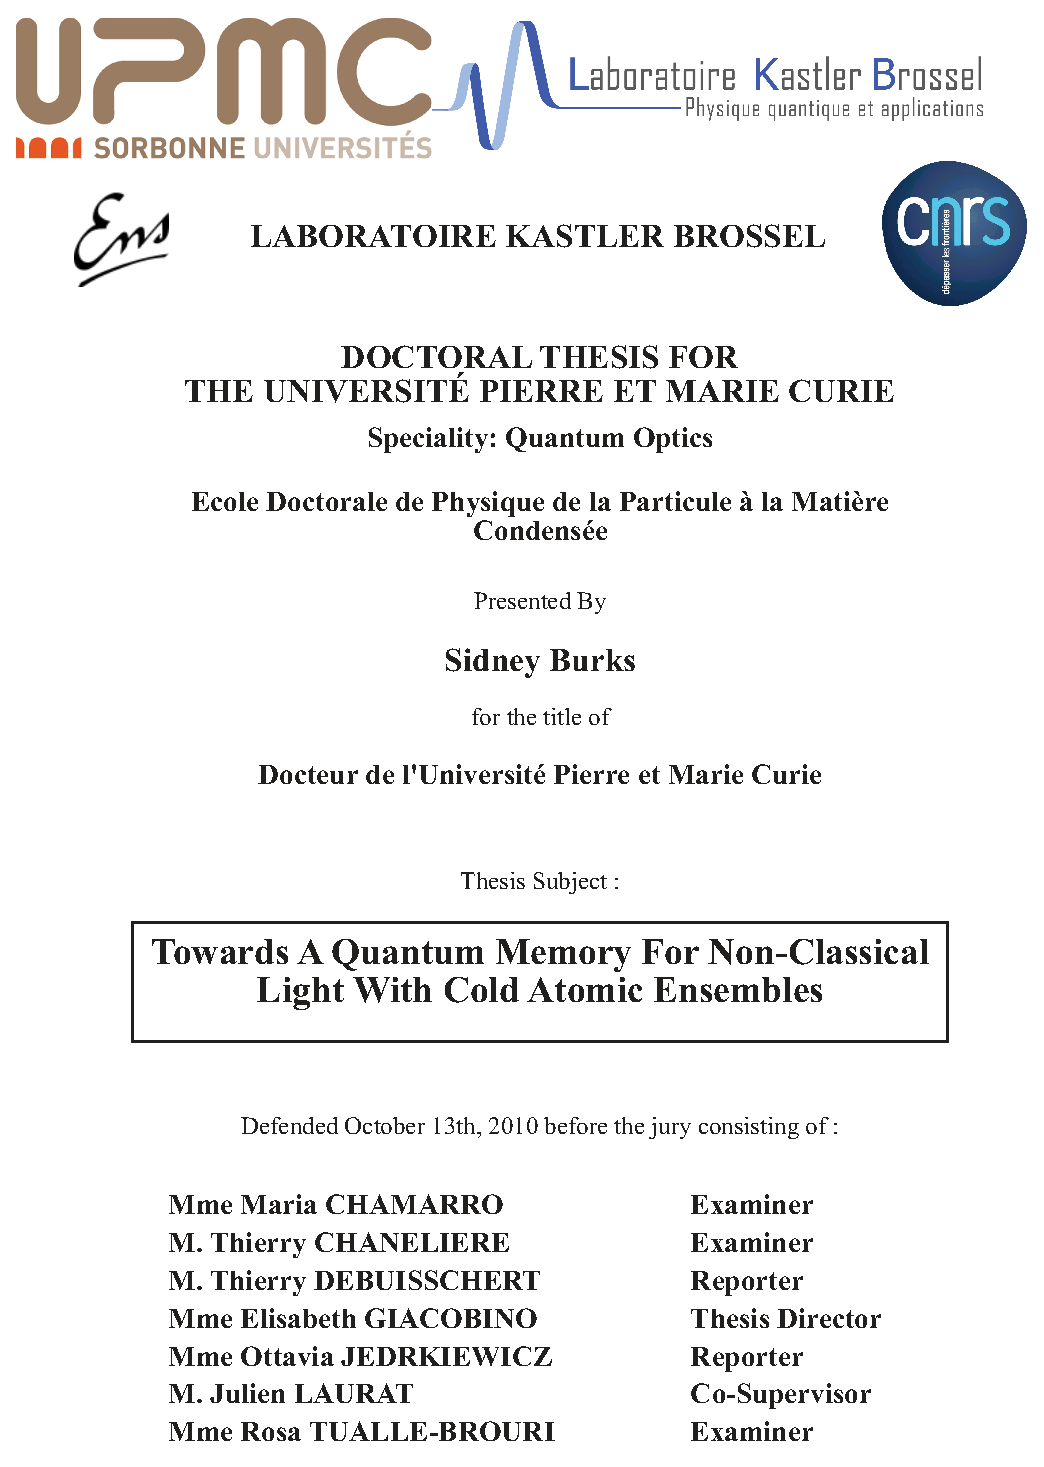
\epsfig{file=cover.eps,width=1.10\textwidth}
$$
\end{figure}

%% 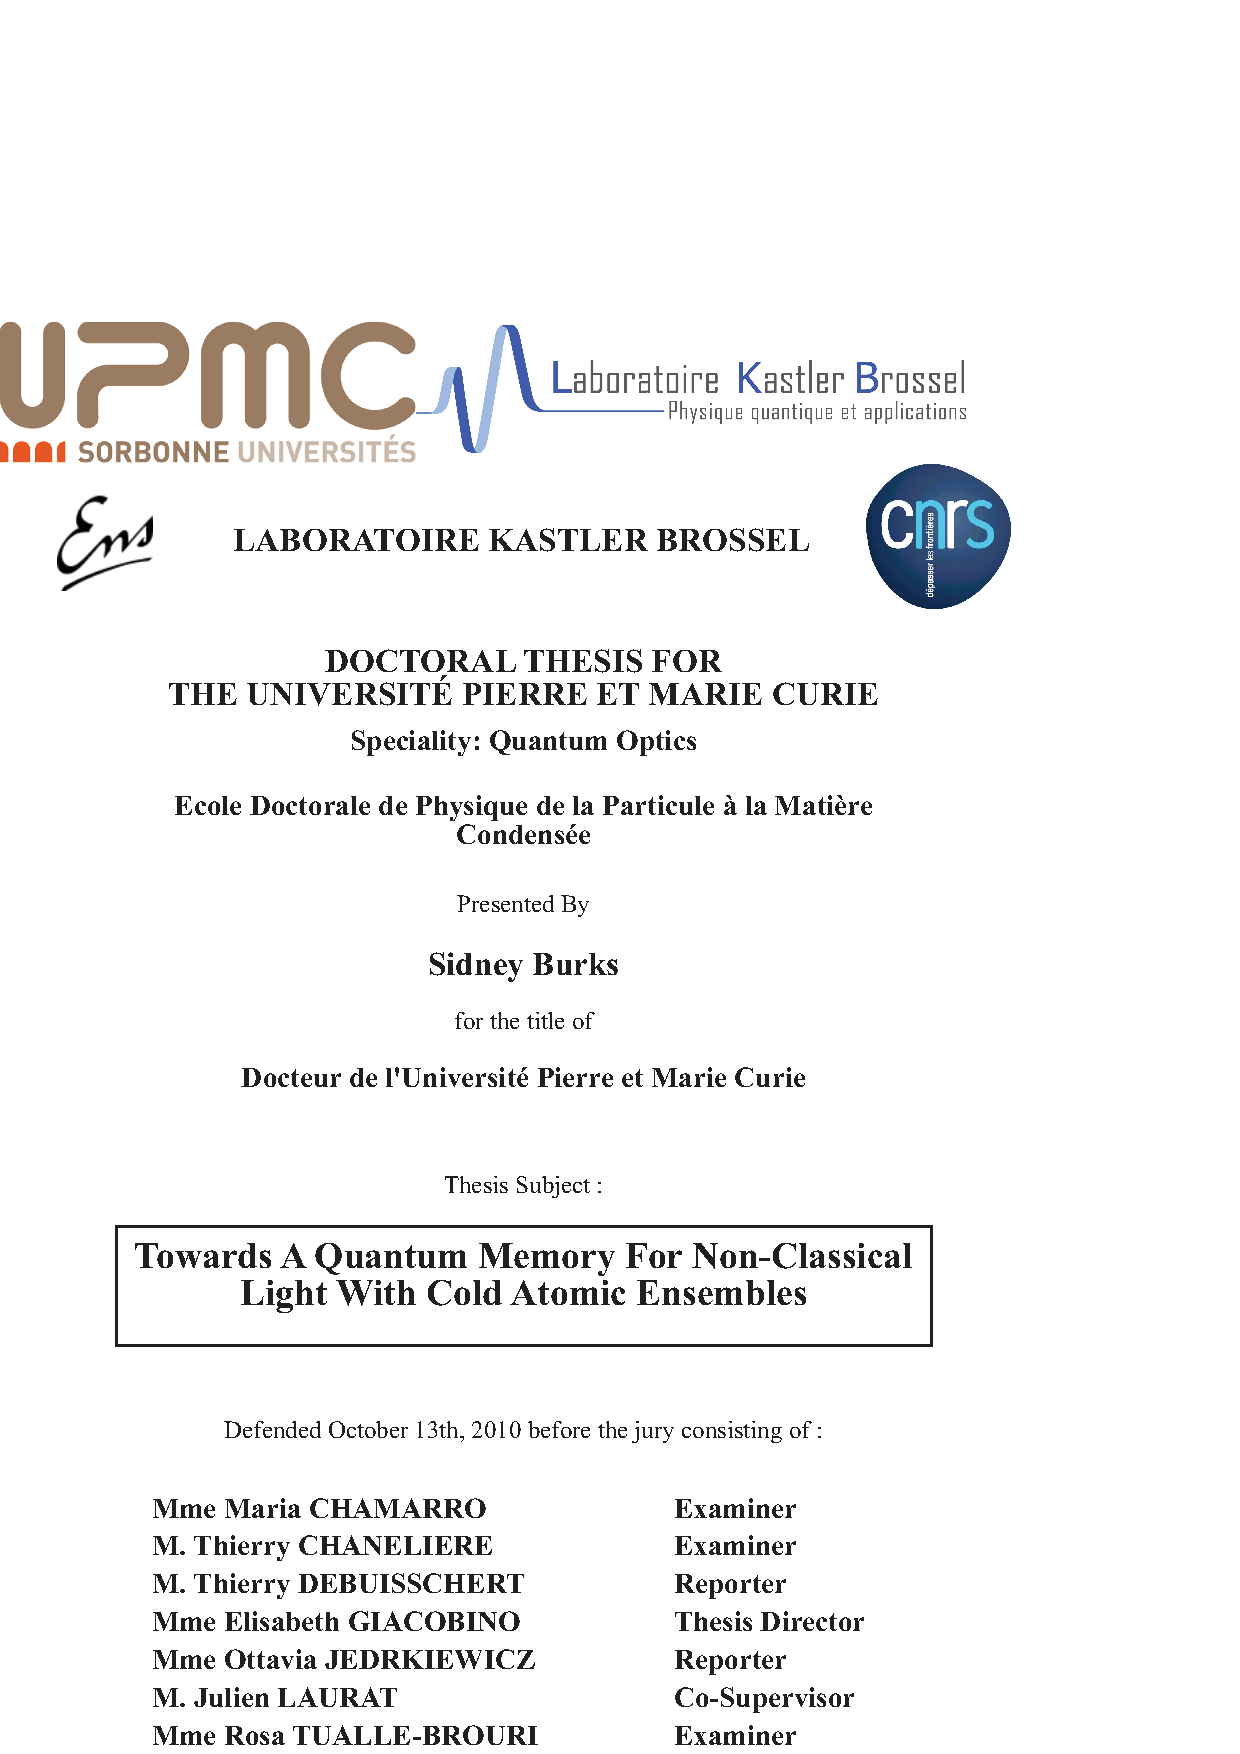
\includepdf{cover}
\newpage
\thispagestyle{empty}
\newpage
\null
\cleardoublepage

\setlength{\textwidth}{155mm}  
\setlength{\oddsidemargin}{5mm}
\setlength{\textheight}{208mm}
\setlength{\evensidemargin}{0mm}

%%%%%%%%%%
% RESUME %
%%%%%%%%%%
\thispagestyle{empty} 

\resizebox{!}{0.05mm}{.}

\vspace{-2cm}

\paragraph{Abstract}
\ \vspace{1.4ex}
\\
\indent
A reversible quantum memory allowing us to store and retrieve quantum information serves as a key necessity for implementing many of novel quantum information protocols. As light serves as a reliable long-range carrier of quantum information, and atoms offer the possibility of long storage times, current attempts at creating quantum memories focus on the transfer of the quantum fluctuations of light onto atomic coherences.  The work in this thesis focuses on the development of a quantum memory for squeezed light using an ensemble of cold Cesium atoms stored in a magneto-optical trap.  Our two major milestones were the development of a source of nonclassical light, and the development of a suitable atomic medium for storage.

We first present the results of our efforts to generate a source of squeezed vacuum states resonant with the Cesium $D_2$ line using a PPKTP nonlinear crystal inside of an optical parametric oscillator.  Additionally, we characterize these squeezed states by carrying out a quantum state tomography using an iterative maximum likelihood approach.

Next we look at the development of a new experiment which would allow us to use cold Cesium atoms as a storage medium in our recently developed magneto-optical trap. As this requires an array of novel tools and experimental techniques, we will discuss the development of these elements, and how they have furthered our progress towards storing quantum states onto our Cesium atoms, and eventually entangling two atomic ensembles.



\vspace{0.5cm}

\noindent{\bf Keywords:} quantum optics, quantum information, continuous variables, quantum memory, optical parametric oscillator, squeezed states, entanglement, quantum tomography, electromagnetically induced transparency, cesium vapor.



\vspace{5mm}
\newpage
\thispagestyle{empty}
\newpage
\null
\cleardoublepage
\thispagestyle{empty}
\paragraph{R�sum�}
\ \vspace{1.4ex}
\\
\indent
Une m�moire quantique r�versible permettant de stocker et relire de
l'information quantique est une composante majeure dans la mise en oeuvre de
nombreux protocoles d'information quantique.  Comme la lumi�re est un porteur de
l'information quantique fiable sur des longues distances, et comme les atomes
offrent la possibilit� d'obtenir de longues dur�es de stockage, le recherche
actuelle sur la cr�ation d'une m�moire quantique se concentre sur la transfert
des fluctuations quantiques de la lumi�re sur des coh�rences atomiques.  Le
travail r�alis� durant cette th�se porte sur le d�veloppement d'une m�moire
quantique pour la lumi�re comprim�e, utilisant un ensemble d'atomes froids de
C�sium stock�s dans un pi�ge magn�to-optique.  Nos deux principaux objectifs
�taient le d�veloppement d'une source de lumi�re non-classique, et le d�veloppement d'un millieu atomique pour le stockage de celle-ci.


Tout d'abord, nous commen�ons par pr�senter la construction d'un oscillateur
param�trique optique qui utilise un cristal nonlineaire de PPKTP.  Cet OPO
fonctionne comme source d'�tats de vide comprim� r�sonant avec la raie $D_2$ du Cesium.  Nous caract�risons ces �tats gr�ce � une reconstruction par tomographie quantique, en utilisant une approche de vraisemblance maximale.

Ensuite, nous examinons une nouvelle exp�rience qui nous permet d'utiliser comme
millieu de stockage des atomes froids de C�sium dans un pi�ge magneto-optique
r�cemment d�velopp�.  Car cette exp�rience exige l'utilisation de nouveaux
outils et techniques, nous discutons le d�veloppement de ceux-ci, et comment ils
ont contribu� � notre progression vers le stockage des �tats quantiques dans nos
atomes des C�sium, et finalement vers l'intrication de deux ensembles atomiques.

\vspace{0.5cm}

\noindent{\bf Mots cl�s:} optique quantique, information quantique, variables continues, m�moire quantique, transparence induite �lectromagn�tiquement, vapeur de c�sium, oscillateur param�trique optique, �tats comprim�s, intrication, tomographie quantique.

\newpage
\thispagestyle{empty}

\null
\addtolength{\textheight}{20mm}
\cleardoublepage
\pagestyle{empty} 
\addtolength{\parskip}{5 pt}

\begin{center}
\textbf{\large Acknowledgements}
\end{center}

\noindent
The work presented in this thesis results from the passionate efforts and support of many people, without whom none of the following results would have come into fruition.

\noindent
I would like to begin by thanking Elisabeth Giacobino and Alberto Bramati for allowing me to join their Quantum Optics group and take part in their research.  

\noindent
An enormous thank you to Julien Laurat, who has supported me in every aspect of this work with his patience, encouragement, and trust, from the beginning through the end, and really made this work a success.

\noindent
I would particularly like to thank Maria Chamarro, Thierry Chaneli\`ere, and Rosa Tualle-Brouri for accepting to take the time and effort to serve on the jury, alongside Ottavia Jedrkiewicz and Thierry Debuisschert, who have additionally agreed to serve as reporters for this thesis,

\noindent
Antonino Chuimmo for introducing me to the OPO, and patiently teaching me as much as he possibly could in the short month we worked together,  

\noindent
Jean Cviklinski for acting as a role model of a researcher,  

\noindent
Jeremie Ortalo for his dedication in working with me side-by-side through all of the long hours developing the experiment for two years,

\noindent
Xiaojun Jia for his insights on solving many of our problems in constructing the OPO,

\noindent
Michael Scherman, Pietro Lombardi, Lambert Giner, and Lucile Veissier, and Oxana Mishina for all of their insights and disscussion surrounding the experiment,

\noindent
Jurgen Appel for his help with implementing the optical phase lock,

\noindent
Bridgitte Delamour for her passion, attention to detail, and professionalism she put into her work,

\noindent
Jean-Piere Okpisz for his excitement in developing new solutions to problems,

\noindent
Mohammed Boujrad for working with me in developing microcontroller and FPGA based tools for our research,

\noindent
Jean-Michel Isac, Pascal Travers, Alain Vogt, Chrisophe Rafaillac, Gael Coupin, and Arnaud Leclercq for their precision, diligence, and skill in creating new mechanical devices,

\noindent
Eric LeBigot, Virginia  D'Auria, Pierre Cladet, Benoit Chalopin, Olivier Pinel and Taoufik Amri for showing me other aspects of quantum optics beyond my immediate research,

%\noindent
%Monique Bonnamy, Laetitia Morel, Genevieve Leonis for all of the administrative duties that they carried out,

\vspace{20 pt}
\noindent
My family for always pushing me to follow my dreams,

And most importantly, Elodie Culoma, my Sweetiedumonde, for being the most loving, patient, supportive sweetiedumonde ever.

\addtolength{\parskip}{-5 pt}
\addtolength{\textheight}{-20mm}
\rmfamily\normalfont
\cleardoublepage


\pagestyle{fancy}

\pdfbookmark[0]{Table of Contents}{toc}
\tableofcontents

\cleardoublepage
\phantomsection  
\pdfbookmark[0]{List of Figures}{fig}
\listoffigures
\mainmatter
 
\chapter*{Introduction}
\addstarredchapter{Introduction}
\markboth{Introduction}{}
\label{introduction} 


\subsection*{Quantum Information vs. Classical Information}

The field of Quantum Information has developed rapidly over the last few
decades.  Quantum Mechanics has allowed us to manipulate light and matter in new ways, permitting us to observe phenomenon that have no classical parallel.  Many of
these phenomenon arise due to core quantum principles such as the Heisenberg
Uncertainty Principle, and the superposition of states.  As a result, this has led to a shift from our classical definitions of information towards the concept of quantum information.  The fundamental element at the core of
quantum information is the quantum bit, or \emph{qubit}.  While classical bits
allow us to represent information as discrete values of 1 or 0, qubits take
advantage of quantum superposition, which allows them to represent information as 1, 0, or a superposition of both values.

This characteristic of qubits has led to the development of novel protocols
concerning information transfer, calculation, and computation that are
impossible to implement when only considering classical bits of information.  One of the first insights on ways to benefit from using quantum information was proposed by Feynman in 1981, when he suggested that we use a quantum computer to
simulate the evolution of quantum systems \cite{feynman1982simulating}.
Shortly afterwards in 1984, Bennett and Brassard developed a protocol to use
secure quantum channels for the distribution of cryptographic keys
\cite{Bennett84}.  This was quickly followed by the work of Deutsch, who
developed the first model of a quantum Turing machine, thus giving us a means to
analyze quantum algorithms using quantum logic gates \cite{Deutsch85}.
In 1991, Ekert continued the exploration of quantum information transfer by
developing a protocol for secure communication based on quantum entanglement
\cite{Ekert91}.  Research concerning the usage of quantum information for
calculations continued throughout the 1990s with the development of Shor's
algorithm in 1994, which provided a means to rapidly factor large numbers
using a quantum computer \cite{Shor94}, and Grover's algorithm, which provided a
means of using quantum information to search an unsorted database
\cite{Grover96}. 

All of these protocols concerning the manipulation of quantum information rest
on the premise that we preserve the quantum superposition of our qubits.  Preserving the quantum superposition requires us to avoid measuring the value of a qubit, which would force it to take on a well-defined value and destroy its quantum characteristics.  This poses a problem if we approach these protocols with our classical treatment of information, as quantum mechanics imposes a no-cloning theorem which forbids us from making exact copies of unknown quantum states.  This limitation has sparked the need to develop a new means of preserving quantum information for long-term manipulation and storage.

\subsection*{Quantum Memories}

A reversible quantum memory allowing us to store and retrieve quantum
information serves as a key necessity for implementing many of these quantum
information protocols.  We could for example, use a quantum memory as a
deterministic single-photon source, which would serve as an important element
in optical quantum computing.  Quantum memories would also resolve a critical
problem with the long-distance transfer of quantum information.  The optical
propagation of photons in fiber optic cables is subject to losses, which limits the
distance over which we can transfer optical qubits.  Quantum repeaters could
be developed to bypass this limitation by entangling photons at both ends of
our communications chain, but this is only possible if quantum memories are
used to temporarily store quantum states.  It is this context that has
motivated our group to work towards the development of a quantum memory.



\subsection*{Research at the Laboratoire Kastler-Brossel}

Over the last 20 years, the Quantum Optics group at the Laboratoire Kastler-Brossel has focused on studying the quantum-optical effects of light-matter interactions in Cesium atoms.  There have been a variety of experiments carried out to study the quantum noise reduction in cavities and with cold atoms by Laurent Hilico \cite{HilicoPhD}, Astrid Lambrecht \cite{LambrechtPhD}, Thomas Coudreau \cite{CoudreauPhD}, and Vincent Josse \cite{JossePhD}.  The theses of Laurent Vernac \cite{VernacPhD} and Aurelien Dantan \cite{DantanPhD} have developed the theoretical work concerning quantum electromagnetic fluctuations and their transfer towards atoms via light-matter interactions.  Most recently, the work of Jean Cviklinski \cite{CviklinskiPhD} and Jeremie Ortalo \cite{ortalo} has yielded the development and characterization of an atomic memory for coherent states with warm atoms, and an experimental study of electromagnetically-induced transparency in Cesium.

 

\newpage
\section*{Thesis Outline}

Part \ref{part:1} of this thesis begins with a theoretical overview of the
general quantum optics concepts used to carry out the experimental work shown here.  We define the quantum states of the electromagnetic field, and show how we can represent those states using the density matrix and Wigner function.  We then proceed to discuss the nonlinear optics of light as it passes through a nonlinear material, and show how we can use these interactions to generate squeezed states.

In Part \ref{part:2}, we look at the experimental setup used to create an optical parametric oscillator, which allows us to generate squeezed vacuum states resonant with the Cesium D2 line at 852 nm.  We then look at the techniques used to characterize these states using quantum homodyne tomography and iterative maximum likelihood estimation.  We finish by discussing the approaches that we developed to convert our continuous source of squeezed light into pulses compatible with our quantum memory.

Finally in Part \ref{part:3}, we look at the development of a new experiment which would allow us to use cold Cesium atoms as a storage medium in our recently developed magneto-optical trap.  As this requires an array of novel tools and experimental techniques, we will discuss the development of these elements, and how they have furthered our progress towards storing quantum states onto our Cesium atoms, and eventually entangling two atomic ensembles.

\part{Introduction to Quantum Optics}
\label{part:1} 
\chapter{Motivation for a Quantum Memory}
%4/5 pg
\label{ch:1} 

The aim of a quantum memory is to provide a means of storing information encoded into quantum states, and allow a mechanism for reliable, on-demand retrieval.  As light serves as a reliable long-range carrier of quantum information, and atoms offer the possibility of long storage times, current attempts at creating quantum memories focus on the transfer of the quantum fluctuations of light onto atomic coherences.  We can establish a performance metric for a quantum memory by using measurements such as its storage and retrieval efficiency, the conditional or non-conditional fidelity of its output state as a representation of its input state, the overall storage lifetime, and our ability to store arbitrary quantum states in it.  Other considerations for a quantum memory include the wavelength of light to which it responds, the number of frequential modes we can store inside of it simultaneously, and the bandwidth of light it supports.  Despite current attempts at implementing a quantum memory, as of yet there is no system available that shows a high performance with regards to all of these characteristics.


\section{Applications of a Quantum Memory}

We can define a quantum memory as a coherent and reversible transfer of qubits to and from a storage medium, such that our retrieved state superposition is a faithful representation of the original stored state.

\begin{eqnarray}
  \label{eq:qmem}
  \underbrace{\alpha \ket{0} + \beta \ket{1}}_{\text{Input state}}  \rightarrow \underbrace{\alpha \ket{a} + \beta \ket{b}}_{\text{Stored state}} \rightarrow \underbrace{\alpha \ket{0} + \beta \ket{1}}_{\text{Retrieved state}}.
\end{eqnarray}

\noindent
A quantum memory for light is a necessary component in several systems which would permit the advanced manipulation of quantum information.  

One of the simplest usages of a quantum memory is as an on-demand source of  single photons.  If we create a pair of photons simultaneously using a system such as parametric down-conversion, we can store one of the photons in the quantum memory, and use the detection of the second photon to signal that our memory has been \emph{prepared}.  Once the memory is charged with a photon, we can release it on demand with the assurance that it yields a single-photon state.  

Another usage of a quantum memory would be as a component of a quantum computer.  Current quantum algorithms require the manipulation of entangled qubits, which are often processed in parallel for each step in a computation. We can use a quantum memory as a timing mechanism which stores qubits while other steps of the computation are being prepared so they can be processed at the right moment.  In this way, a quantum memory would serve as a synchronizing tool for quantum computations \cite{lvovsky2009optical}. 

We can also envision the usage of a quantum memory for long-range quantum communication.  The promise of unbreakable quantum communications channels depends on protocols such as quantum key distribution, which require the exchange of qubits over long distances.  Fiber optic cables at the telecom 1550 nm wavelength typically have attenuation levels of 0.25 dB/km, and experiments with the detection of entangled photons has resulted in the detection of around 100 qubits/second \cite{Zeilinger07b}.  Due to attenuation losses, transferring quantum states through fiber optic cables is currently limited to a few hundred kilometers.


Using a quantum repeater protocol illustrated in Figure \ref{fig:q_rep} would
allow us to bypass this limitation \cite{Briegel98}, \cite{Duan01}.  We can
begin by defining two points $A_0$ and $A_N$ separated by a distance L, over
which we would like to entangle two quantum states.  One way to accomplish
this is by first dividing our distance up into N segments.  At the end of each segment, we can place a twin photon source, which we can use to entangle each segment with its neighboring segment.  By entangling each sub-segment with its neighbor, we can swap entanglement over the entire length L.

One problem with this approach however, is that entangling the path extremities via entanglement swapping is a process that must be properly synchronized, so that the entanglement of every segment node happens simultaneously.  This posses a problem because the probability of experiencing an entanglement error in at least one of the nodes increases exponentially as the number of nodes increase, and as a result, so does the time required to simultaneously entangle all nodes. 


\begin{figure}[!ht] 
 \centering 
 \includegraphics[width=0.65\textwidth]{figures/q_rep} 
 \caption[Quantum repeater schematic]{Diagram of the protocol for
distributing photon entanglement between points $A_0$ and $A_N$.  Length L is
divided into N segments, which are connected by quantum repeaters.
Entanglement is shared between segments via entanglement swapping at the
nodes.  a)  Entanglement swapping along the entire length requires perfect
synchronization, and a time exponential in the path length.  b)  Placing a
quantum memory at each node facilitates the synchronization, and reduces the
time to a polynomial time with path length.} 
 \label{fig:q_rep} 
\end{figure}


A solution to this would be to place a quantum memory at each node, which would allow us to temporarily store our entangled photons while the other nodes were being prepared, allowing us to independently entangle each segment.  Once all of the nodes were in a prepared state, we could then carry out the entanglement swapping over the entire distance.  This would lower the probability of error to a polynomial order with increasing distance, as opposed to exponential, thus rendering our long-distance communication practical.  As in the case of quantum computation, a quantum memory makes quantum repeaters practical by synchronizing the entanglement of states.

As these applications all show the potential promise of novel ways to manipulate quantum information, they provide a great motivation for the development of a performant quantum memory.



\section{Research Avenues} 

The last 10 years have seen a large development in the research attempts in
constructing a quantum memory.  Numerous methods exist for preserving the
quantum state of light, but the most promising techniques for longer storage
times are those using large ensembles of atoms.  Work such as that done by
\cite{Kuzmich05}, and \cite{Lukin05} has succeeded in the storage and retrieval of single-photon states.  The work of \cite{Polzik04} has shown the ability to use continuous-variable quantum non-demolition techniques to achieve high efficiencies and storage times in Cesium, yet they have only allowed the retrieval of a single quadrature of light.  Photon-echo techniques have also been explored in order to preserve the atomic coherences, and thus extend the overall memory storage time.  Work done by \cite{PhysRevLett.96.043602} in 2006 using Controlled Reversible Inhomogenous Broadening (CRIB) has been applied in Pr doped solid-state Y$_2$SiO$_5$ crystals cooled to 4 K, however with low efficiency results.  Other photon-echo techniques such as the usage of an Atomic Frequency Comb (AFC) have been demonstrated showing a 9\% storage efficiency of weak photon pulses \cite{chaneliere2010efficient}.  The usage of EIT as a storage mechanism has also yielded results by several groups.  In the work of \cite{choi2008mapping}, entangled states were successfully stored and retrieved from Cesium vapor. Several groups have also succeeded in the storage and retrieval via EIT of coherent states in Cesium vapor \cite{CviklinskiPhD}, and squeezed vacuum states in Rubidium vapor \cite{Lvovsky08}, \cite{Kozuma08}, \cite{Kozuma09}.



\section{Our Approach}

Our approach towards the construction of a quantum memory focuses on the
transfer of squeezed vacuum states onto Cesium cloud trapped and cooled in a
magneto-optical trap (MOT).  We wish to transfer the quadrature fluctuations of the light field onto the collective spin of Cesium atoms stored in an magneto-optical trap, and after the storage time of a few tens of microseconds, re-emit the light to show the preservation of quadrature squeezing.  Once this is accomplished, we aim to carry out the storage in two atomic ensembles, and show the ability of our system to preserve the entanglement of two remote ensembles.


\chapter{Continuous Variable Quantum Optics}
\label{ch:2}
\minitoc

In this chapter, we will review the foundations of quantum mechanics and
quantum optics, and explore the different quantum states of the
electromagnetic field.  We will then examine how to manipulate these quantum
states to produce non-classical correlations in optical beams.

 
\section{Quantum States}
\label{quantum_states} 

The postulates of quantum mechanics give us a way of
defining the state of a system and its observable quantities that is
fundamentally different from that used in
classical mechanics.  The first axiom
says that the state of a system at a fixed time is defined by a state vector
$\ket{\psi}$.  We can represent a state vector as a superposition of basis states by 


\begin{eqnarray}
  \label{eq:quantum_state_decomposition}
  \ket{\psi} = \sum_{n} c_{n} \ket{n} \quad & \quad p_n = \abs{c_n}^2 =
\frac{\abs{\braket{n}{\psi}}^2}{\braket{\psi}{\psi}} \quad & \quad \sum \abs{c_n}^2 = 1 ,
\end{eqnarray}

\noindent
where each of the $c_n$ coefficients represent a complex amplitude of the eigenvector $\ket{n} $, and the probability amplitudes $\abs{c_n}^2$are subject to a normalization condition.  Upon measurement, we have a probability $p_n$ of detecting the system in the state $\ket{n}$.  Within this framework, observable quantities are represented by Hermitian operators $\hat{O}$, whose expected value can be calculated by


\begin{equation}
  \label{eq:observable}
  \avg{\hat{O}}_{\ket{n}} = \sum_n c_n \bra{n} \hat{O} \ket{n}.
\end{equation}


When we know for certain that a system exists within a uniquely given state,
we can refer to this state as a \emph{pure state}, and the state vector
$\ket{\psi}$ encompasses all of the information that we can obtain about the
system.   We can, however, imagine a more general case of a system that is
composed of an ensemble of sub-states $\ket{\psi_n}$, where each sub-state
appears in the ensemble with a probability $P_n$.  We can thus describe this
system, as a \emph{statistical mixture} of pure states, or a \emph{mixed
state}, where

\begin{equation}
  \label{eq:mixes_states_norm}
  \sum_i  P_i = 1.
\end{equation}


\subsection{The Density Operator} 
\label{the_density_operator} 

We can introduce the \emph{density operator} $\hat{\rho}$ as a means of representing a system composed of mixed states, using the expression

\begin{equation}
  \label{eq:density_operator}
  \hat{\rho} = \sum_n P_n \proj{\psi_n}.
\end{equation}

This operator fully describes the quantum state of the system as it
encompasses the complex coefficients for the pure states available to our
system, as well as the fact that we only have probabilistic information $P_n$ about precisely which state our system is in.  Furthermore, the density operator allows us to calculate all of the information that quantum mechanics can provide about the system, whether the system be in a precisely known pure state, or in a statistical mixture of states.



\subsubsection{Properties of the Density Operator}
\label{properties_of_the_density_operator} 

The density operator has several properties which allow us to make predictive measurements about our system.  If we have an Hermitian observable $\hat{O}$, then we can calculate the expectation value of our observable using \cite{cohen} 

\begin{equation}
  \label{eq:observable_from_density}
  \avg{\hat{O}}  = \sum_{n} P_n \matrixel{\psi_n}{\hat{O}}{\psi_n} =
Tr(\hat{O} \hat{\rho}).
\end{equation}

\noindent
The density operator also has the following properties: it is Hermitian, its trace equals 1, and it is positive semi-definite


\begin{eqnarray}
  \label{eq:density_properties}
  \hat{\rho}^\dagger = \rho \quad & \quad    Tr(\hat{\rho})=1      \quad &
\quad     \matrixel{\psi}{\hat{\rho}}{\psi}   =  \sum_n P_n
|\braket{\psi}{\psi_n}|^2  \ge 0.
\end{eqnarray} 

\noindent
We can use the density operator to distinguish between pure states and mixed states by using the \emph{purity}, which is given by \cite{gerry2005introductory} 

\begin{equation}
  \label{eq:purity_density}
  Tr(\hat{\rho}^2) \quad \quad \text{with } Tr(\hat{\rho}^2) \le 1. 
\end{equation} 

\noindent
The equality holds only when the state is a pure state, whereas for mixed
states, $Tr(\hat{\rho}^2) < 1$.  Furthermore, by using \req{eq:von_neumann} and the system's Hamiltonian $\mathcal{H}$, we can determine the dynamic properties of our system 

\begin{equation}
  \label{eq:von_neumann}
  i \hbar \pd{\hat{\rho}}{t} = [\mathcal{H}, \hat{\rho}].
\end{equation}

\noindent
A complete specification of $\hat{\rho}$ allows us to determine the values of all measurable quantities allowed by quantum mechanics.  For this reason, we consider the density operator as the most general representation of a quantum state.


\subsection{The Wigner Representation}
\label{the_wigner_representation} 


Although the density operator $\hat{\rho}$ provides the most general representation of a quantum state, it still remains an abstract concept which provides us with little intuition about the information contained in a system's state.  We can seek a more illustrative representation of the information contained in the density matrix by using the \emph{Wigner Function} \cite{Wigner32}.

The Wigner function has its conceptual origins in classical and statistical physics, where for a classical statistical ensemble, it is possible to specify the state of the system by precise, simultaneous measurements of its conjugate phase space variables $q$ and $p$ \cite{schleich2001quantum}.  A measurement of these variables would allow us to create a phase-space probability distribution $\wigner$, which would permit the prediction of any other quantities related to the system. 

An attempt to similarly predict the quantities involved with a quantum system
is not as straightforward however.  Quantum mechanics prevents us from
carrying out the precise, simultaneous measurement of $q$ and $p$ due to their non-commutativity, thus there is no way to create a \emph{true} quantum phase space distribution for our system.

Instead of using a true phase space distribution, we can suppose that there
exists a function $\wigner$ which acts like join probability distribution for
$q$ and $p$.  The Wigner function fits this characteristic, and allows us to relate the system's density matrix to a quasi-probability distribution through the following definition \cite{schleich2001quantum}:

\begin{equation}
  \label{eq:wigner_function}
  \wigner = \frac{1}{2\pi \hbar} \intind e^{-\frac{i}{\hbar}p \xi}
\matrixel{q+\frac{1}{2}\xi}{\hat{\rho}}{q-\frac{1}{2}\xi} d\xi.
\end{equation}

\noindent
We can express the Wigner function for a state as a Fourier transform of its density matrix, and in the cases of pure states where $ \dens =  \proj{\psi}$ and given the wavefunction $\psi(x) = \braket{x}{\psi}$, we can express it as a Fourier transform of position-shifted wavefunctions

\begin{equation}
  \label{eq:wigner_pure}
  \wigner = \frac{1}{2\pi \hbar} \intind e^{-\frac{i}{\hbar}p \xi} \;
\psi^*\left(q-\frac{1}{2}\xi\right)\psi \left(q+\frac{1}{2} \xi \right) \;
d\xi.
\end{equation}

\noindent 
We can define the \emph{marginal distributions} as the true probability
distributions of $q$ and $p$ individually.  By integrating $\wigner$ over $q$
or $p$, we can obtain these marginal distributions for $q$ and $p$ respectively \cite{leonhardt1997measuring} 

\begin{eqnarray}
  \label{eq:marginals}
  W(q) = \intind \wigner \; dp    & \quad \text{and} \quad  &   W(p) = \intind
\wigner \;   dq.
\end{eqnarray}

\noindent
These marginals serve as projections of the Wigner function onto the axis of
our $q$ and $p$ coordinates, thus while we cannot measure the entire Wigner function at once, we can measure the marginal projections of it.  

\subsubsection{Properties of the Wigner Function}
\label{properties_of_the_wigner_function} 

The Wigner function has certain properties that make it useful for describing quantum states \cite{schleich2001quantum} .  It acts like a probability distribution through its normalization constraint

\begin{equation}
  \label{eq:normalized_wigner}
  \intind \intind \wigner \; dq \; dp = 1,
\end{equation}

\noindent
and it is purely real for Hermitian operators $\dens$ , such that
 \begin{equation}
   \label{eq:wigner_is_real}
   \wigner^* = \wigner.
 \end{equation}

\noindent
Additionally, $\wigner$ satisfies a trace rule, which allows us to evaluate the overlap of two density operators 

\begin{equation}
  \label{eq:wigner_overlap}
  Tr(\dens_1 \dens_2) = 2 \pi \hbar \intind \intind \;
\mathcal{W}_{\dens_1}(q,p) \; \mathcal{W}_{\dens_2}(q,p) \; dq \; dp.
\end{equation}

\noindent
Using this trace rule, we can once again evaluate the expectation value of an operator $\hat{O}$ using

\begin{equation}
  \label{eq:wigner_expectation}
  \avg{\hat{O}} =  Tr(\dens \hat{O}) = 2 \pi \hbar \intind \intind \;
\mathcal{W}_{\dens}(q,p) \; \mathcal{W}_{\hat{O}}(q,p) \; dq \; dp,
\end{equation}

\noindent
or similarly, we can determine the purity $Tr(\dens^2)$ of a state by


\begin{eqnarray}
  \label{eq:wigner_purity}
  Tr(\dens^2) \le 1    & \Rightarrow & 2 \pi \hbar \intind \intind \;
\mathcal{W}^2_{\dens}(q,p) \; dq \; dp \le 1.
\end{eqnarray}

\noindent
The Wigner function is positive when describing Gaussian states, but can take on negative values when we use it to describe non-gaussian states.  When $\wigner < 0$, we interpret this as a strong signature of non-classical behavior.  Because of its ability to take on negative values under certain conditions, we consider it to be a \emph{quasiprobability} distribution as opposed to a true probability distribution.

Finally, the overlap formula allows us to express the density matrix in terms of the Wigner function in a given basis by using the relation shown in \cite{leonhardt1997measuring}

\begin{equation}
  \label{eq:wigner_to_density}
  \matrixel{\psi_a}{\dens}{\psi_b} = Tr(\dens \ket{\psi_b}\bra{\psi_a}) = 2
\pi \hbar \intind \intind \wigner \mathcal{W}_{\psi_a \psi_b}(q,p) \; dq \;
dp.
\end{equation}

\noindent
These properties shows us that we can treat the Wigner function as a true representation of a quantum state, and use it for the calculation of relevant quantities.



% Electric Field
\section{Quantum States of the Electric Field} 
\label{quantum_states_of_the_electric_field} 

Light serves as an extremely useful tool in the study of quantum states, and
the development of lasers over the last 50 years has allowed us to easily
create highly coherent sources of light.  By using these light sources, we can
easily encode information and transmit it over long distances.  Additionally, as light is well understood in the classical domain, by studying its uniquely quantum properties we can further our understanding of quantum mechanics.  

In the previous section, we have reviewed several means of describing the quantum states of a system.  Here, we will begin to apply this formalism to the electromagnetic field.  First, we will begin with a classical description of the electric field, and show how through its quantization, it is possible to produce uniquely quantum states of light whose properties have no classical analogues.  

We begin with the classical expression for a single mode electric field:

\begin{equation}
  \label{eq:classical_e_field}
  E(t) = \abs{E_{0}} cos(\omega t + \phi )  = E_1 cos(\omega t) + E_2
sin( \omega t).
\end{equation}

\noindent
Through this description, we see that we have two canonical variables available for describing the E-field: either the field amplitude $E_0$ and phase $\phi$,  or the quadrature components of the field $E_1$, and $E_2$.
  
We can develop a similar quantum expression for the E field by replacing the classical quadratures with quantum operators

\begin{equation}
  \label{eq:quantum_e_field}
     \hat{E}(t) = \hat{E}_1 \cos(\omega t) + \hat{E}_2 \sin (\omega t).
\end{equation}

\noindent
By using the non-commuting photon annihilation and creation operators $\ani$ and $\crea$, we can rewrite these quantum quadrature operators in the form

\begin{eqnarray}
  \label{eq:quad_bosonic_decomposition}
  \hat{E}_{1} = \hat{a} + \hat{a}^{\dagger }  \quad  & \quad    \hat{E}_{2} =
i (\hat{a}^{\dagger } - \hat{a})   \quad  & \quad    [\hat{a},
\hat{a}^{\dagger }] = 1.
\end{eqnarray}

\noindent
When performing measurements on our state, it is useful to specify our measurements in terms of a \emph{generalized quadrature} $\hat{X}_\theta $, which is a linear combination of our two quadrature operators $\hat{E}_{1}$ and $\hat{E}_{2}$ \cite{Fabre90}

\begin{equation}
  \label{eq:generalized_quadratures}
  \hat{X}_\theta = \hat{E}_1 cos \theta + \hat{E}_2 sin \theta = \hat{a} e^{-i
\theta } + \hat{a}^{\dagger} e^{i \theta}.
\end{equation}

\noindent
Through the commutation relation of the boson operators given in Equation \ref{eq:quad_bosonic_decomposition}, we can derive the commutation relationship for the field quadratures, and see that they do not commute

\begin{equation}
  \label{eq:quadrature_commutation}
  \commutator{\hat{E}_1}{\hat{E}_2}=2i.
\end{equation}

\noindent
The non-commutativity of these two quadratures tells us that any simultaneous measurement on them both will only result in a limited precision measurement, which we can quantify by defining the \emph{variance} of our measure as

\begin{equation}
  \label{eq:variance_definition}
  \var{\hat{E}_i} = \avg{\hat{E}^2_i} - \avg{\hat{E}_i}^2.
\end{equation}

\noindent
We can then use the generalized uncertainty principle given in
\req{eq:quadrature_commutation} to derive an uncertainty relationship between the two quadrature variances

\begin{equation}
  \label{eq:HUP}
  \std{\hat{A}} \std{\hat{B}} \ge \frac{1}{2i} \avg{\commutator{\hat{A}}{\hat{B}}}.
\end{equation}

\noindent
Using \req{eq:quadrature_commutation} with this uncertainty relation tells us
that any simultaneous measurement of the two quadrature components will yield a
certain amount of imprecision in the measurement.  Thus, the result of our measurement will be subjected to a \emph{quantum noise}.

\begin{equation}
  \label{eq:quadrature_hup}
  \std{\hat{E}_1} \std{\hat{E}_2} \ge 1.
\end{equation}



%%% Quantum States

% Vacuum
\subsection{Vacuum States}
\label{vacuum_states} 

Now that we have a quantum expression for the electric field, we can begin to
look at the quantum optical states that we can produce.  The most fundamental
state is the vacuum state $\ket{0}$, which is a purely quantum state that has no classical analogue.  The mean number of photons $\avg{\hat{n}}$ in the vacuum state is $0$, however because we cannot violate the uncertainty principle given above, the variances of the photon number can never go to $0$

\begin{eqnarray}
  \label{eq:vacuum}
  \avg{\hat{n}} = \bra{0} \hat{n} \ket{0} = 0   \quad & \text{and} \quad  & \std{\hat{E}_1} = \std{\hat{E}_2} = 1.
\end{eqnarray}

\noindent
This restriction tells us that even in the vacuum state with an average photon number of $0$, we observe noise fluctuations in our quadrature measurements.  The vacuum state has symmetric variances in both quadratures, which allows it to satisfy the equality given by \req{eq:quadrature_hup}.  By satisfying this equality, we can call this state a \emph{minimum uncertainty} state whose noise fluctuations are at the \emph{standard quantum limit} (SQL).  We can express the Wigner function for the vacuum state by \cite{leonhardt1997measuring}

\begin{equation}
  \label{eq:wigner_vacuum}
  \wigner = \frac{1}{\pi} e^{-q^2-p^2}.
\end{equation}




% Number
\subsection{Fock States}
\label{fock_states} 

The next set of states that we can consider are the Fock or \emph{number} states \cite{fox2006quantum}.  The Fock state represents a state that contains a precisely well-defined number of photons, thus a completely undefined phase. We can define the number operator $\hat{n}$ in terms of the annihilation and creation operators

\begin{equation}
  \label{eq:number_operator}
  \hat{n}= \crea \ani.
\end{equation}

\noindent
The action of the number operator on a number state vector gives us the number of photons present in that state, and shows us that the variance of the photon number is 0

\begin{eqnarray}
  \label{eq:n_equation_phase}
  \hat{n}\ket{n} = n \ket{n}  \quad & \text{and} \quad & \text{Var}(\hat{n}) = 0.
\end{eqnarray}

\noindent
Fock states containing photons have symmetric noise variances, but are not minimum uncertainty states

\begin{equation}
  \label{eq:number_properties}
  \std{\hat{E}_1} = \std{\hat{E}_2} = \sqrt{2n+1}.
\end{equation}
 
\noindent
We can express the Fock state for a given photon number as a series of photon creation operations acting on the vacuum state.

\begin{equation}
  \label{eq:number_state}
  \ket{n} = \frac{\hat{a}^{\dagger n}}{\sqrt{n!}}\ket{0}.
\end{equation}

\noindent
The Fock states have a Wigner function given by

\begin{equation}
  \label{eq:wigner_fock}
  \wigner = \frac{(-1)^n}{\pi} e^{-q^2-p^2}L_n(2q^2+2p^2),
\end{equation}

\noindent
where the $L_n(x)$ represent the Laguerre polynomials \cite{leonhardt1997measuring}.



% Coherent
\subsection{Coherent States}
\label{coherent_states} 

Mathematically, we can construct a coherent state by applying the
\emph{displacement operator} $ \hat{D}(\alpha)$ to the vacuum state $\ket{0}$
\cite{scully1997quantum}.  Coherent states $\ket{\alpha} $ are considered as quantum states which most closely resemble classical states

\begin{equation}
  \label{eq:displacment_operator}
  \hat{D}(\alpha) = e^{\alpha \crea - \alpha^* \ani} = e^{\frac{1}{2}\abs{\alpha}^2 }e^{\alpha \crea}e^{-\alpha^* \ani}
\end{equation}



\begin{equation}
  \label{eq:displaced_vacuum}
  \hat{D}(\alpha) \ket{0} = \ket{\alpha}.
\end{equation}

\noindent
We can use Equation \ref{eq:displacment_operator} to express the coherent states as an expansion of Fock states \cite{Glauber63} 

\begin{equation}
  \label{eq:coherent_fock_expansion}
  \ket{\alpha} =  e^{-\frac{\abs{\alpha}^2}{2}} \sum_n \frac{\alpha^n}{\sqrt{n!}} \ket{n}.
\end{equation}
 
\noindent
We can also calculate the probability of a coherent state having a given number of photons $P(n)$, and we see that this probability follows \emph{Poisson} statistics \cite{fox2006quantum}.  Thus due to our ability to approximate classical states with coherent states, we can define classical states of light as having Poissonian statistics

\begin{equation}
  \label{eq:coherent_probability}
  P(n) = \abs{\braket{n}{\alpha}}^2 = \frac{\abs{\alpha}^{2n}e^{-\abs{\alpha}^2}}{n!}
\end{equation}

\noindent
As \req{eq:coherent_equation} shows, we can express coherent states as
eigenstates of the annihilation operator $\ani$

\begin{equation}
  \label{eq:coherent_equation}
  \ani \ket{\alpha} = \alpha \ket{\alpha }.
\end{equation}

\noindent
Coherent states have equal variances in their quadratures, and an optical beam composed of coherent states has a mean number of photons that is proportional to its intensity $\abs{\alpha}^2$

\begin{eqnarray}
  \label{eq:coherent_properties}
    \std{\hat{E}_1} = \std{\hat{E}_2} = 1   \quad & \quad \std{\hat{n}} =  \abs{\alpha} \quad & \quad \avg{\hat{n}} = \abs{\alpha}^2.
\end{eqnarray}

\noindent
The Wigner function of a coherent state is given by \req{eq:wigner_coherent}

\begin{equation}
  \label{eq:wigner_coherent}
  \wigner = \frac{1}{\pi} e^{-(q-q_0)^2-(p-p_0)^2}.
\end{equation}


\begin{figure}[!ht] 
 \centering 
 \includegraphics[width=0.45\textwidth]{figures/wigner_coherent} 
 \caption[Wigner function for Coherent state]{Wigner function depicting a coherent state} 
 \label{fig:wigner_coh} 
\end{figure}

% Squeezed
\subsection{Squeezed States}

Squeezed states are another example of purely quantum states.  We can create a squeezed state through the action of the squeezing operator \cite{garrison2008quantum}

\begin{equation}
  \label{eq:squeezing_operator}
  \hat{S}(\zeta) = e^{\frac{1}{2} (\zeta^* \ani^{2} - \zeta \hat{a}^{\dagger 2}) },
\end{equation}

\noindent
where we define $\zeta$ as the squeezing parameter

\begin{equation}
  \label{eq:squeezing_parameter}
  \zeta = r e^{i \phi }.
\end{equation}

\noindent
Squeezed states respect the uncertainty principle in that the product of the quadrature variances has a minimum value, however, the quadrature variances are not equal.   Thus, we can obtain a variance in one quadrature measurement that goes below the standard quantum limit, at the expense of an increased variance in the other measurement.  Squeezed states have a mean photon number that is a function of the magnitude of squeezing parameter $r$, and $\abs{\alpha}^2$ where $\alpha = \avg{\ani}$ \cite{gerry2005introductory}


\begin{eqnarray}
  \label{eq:squeezed_properties}
    \std{\hat{E}_1} = e^{-r} \quad & \quad \std{\hat{E}_2} = e^{r}   \quad & \quad  \avg{\hat{n}} = \abs{\alpha}^2 + sinh(r).
\end{eqnarray}

\noindent
One important type of squeezed state that we will discuss is the squeezed vacuum, whose Wigner function we can express with \cite{leonhardt1997measuring}

\begin{equation}
  \label{eq:wigner_squeezed_vacuum}
  \wigner = \frac{1}{\pi} exp(-e^{2\zeta}q^2-e^{-2\zeta}p^2).
\end{equation}


\begin{figure}[!ht] 
 \centering 
 \includegraphics[width=0.45\textwidth]{figures/wigner_sqz} 
 \caption[Wigner of Squeezed State]{Wigner function for a squeezed state
 representing -2.6 dB of quadrature squeezing} 
 \label{fig:wigner_sqz} 
\end{figure}

\subsection{Operator Linearization}  
\label{sec:linearization}

We can linearize our quantum operators by decomposing them into a steady-state classical term, and a fluctuating term, and assuming that the classical term has a much larger amplitude than the fluctuating term \cite{Fabre90}.  If we take the annihilation and creation operators $ \ani$ and $\crea$ as examples, we can represent them in the following form

\begin{eqnarray}
  \label{eq:linearized}
  \ani(t)  & = &  \alpha + \delta \ani(t) \\
  \crea(t) & = & \alpha^* + \delta \crea(t) \\
  \abs{\alpha} & \gg & \abs{\delta \ani(t)}.
\end{eqnarray}

In this decomposition, the first term $\alpha$ represents a classical value, which is the time-averaged value $\avg{\ani}$ of the annihilation operator, and the second term $\delta \ani(t)$ represents the first order fluctuation where we assume that the mean value of the fluctuating term is zero.

This technique provides us with an alternative decomposition of our quantum operators, which can often allow us to solve many problems using analytical approaches.  By using this decomposition, we can express our noise variance directly as a function of our fluctuating term

\begin{equation}
  \label{eq:noise_fluctuation}
  \left(\Delta \hat{O} \right)^2 = \avg{(\delta \hat{O})^2}.
\end{equation}

\subsection{Noise Characterization} 
\label{noise_characterization} 

One problem with using the variance directly for characterizing noise can arise in a case where the variance diverges, such as when we measure white noise.  This divergence occurs due to high-frequency fluctuations in our signal.  In practice, our measurement of noise takes place over a finite frequency bandwidth which filters our noise spectrum.  We can thus obtain a more precise characterization of our noise for a quadrature $\hat{X}(t)$ by using the autocorrelation function \cite{courty05}

\begin{equation}
  \label{eq:autocorelation}
  C_{\hat{X}}(\tau) = \avg{ \delta \hat{X}(t) \delta \hat{X}^\dagger(t')}.
\end{equation}

\noindent
When $C(\tau)$ only depends on the time difference between two instants such that $\tau=t-t'$, we can take the Fourier transform of the autocorrelation function to obtain the noise spectral density

\begin{equation}
  \label{eq:noise_spectral_density}
  S_{\hat{X}}(\Omega ) = \intind C_{\hat{X}}(\tau) e^{i \Omega \tau}  d\tau.
\end{equation}

\noindent
We can relate the autocorrelation function of our Fourier-transformed quadrature to the noise spectral density with 

\begin{equation}
  \label{eq:noise_spectral_fourier}
  \avg{ \delta \hat{X}(\Omega ) \delta \hat{X}^\dagger(\Omega')} = 2 \pi S_{\hat{X}}(\Omega ) \delta(\Omega - \Omega' ).
\end{equation}


\section{Quantum Correlations}
\label{quantum_correlations} 


One phenomenon that we can observe in the quantum domain is the existence of non-classical correlations for a system.  The production of purely quantum states of light aides us in the experimental observation of these correlations.  Here we will show how using a simple tool such as a beamsplitter, and squeezed light will allow us to produce two entangled beams that exert non-classical correlations.

\subsection{Separability Criterion} 
\label{separability_criterion} 

There are many criteria that can be used to determine if correlations between
quadratures are of quantum origin \cite{treps2005criteria}, such as gemellity
as shown in \cite{Giacobino87}, quantum non-demolition measurements, inseparability, and EPR criteria \cite{Reid88}.  Of these we will consider the inseparability criterion for our experiment here.

We define two entangled, or inseparable, systems as systems where it is impossible to factor the two states $\dens_{i1}$ and $\dens_{i2}$ into the independent form 

\begin{equation}
  \label{eq:seperable}
  \dens = \sum_i p_i \dens_{i1} \otimes  \dens_{i2}
\end{equation}

\noindent
Duan \cite{duan} and Simon \cite{simon} established a criterion which allows us to more easily experimentally determine the separability of two states, using 


\begin{equation}
  \label{eq:separability}
  Var(\hat{X}_1 + \hat{X}_2) + Var(\hat{P}_1 -\hat{P}_2) < 2     ,
\end{equation}

\noindent
where $\hat{X}_i$ and $\hat{P}_i$ represent the non-commuting conjugate
operators of system $i$. If the variances of our operators $\hat{X}_i$ and
$\hat{P}_i$ satisfy \req{eq:separability}, we can say that the states are inseparable, and thus exhibit quantum correlations between them.  

\subsection{States Incident on a Beamsplitter} 
\label{states_incident_on_a_beamsplitter} 

With this criterion in place, we can study the properties of two fields incident on a 50/50 beamsplitter.

\begin{figure}[!ht] 
 \centering 
 \includegraphics[width=0.30\textwidth]{figures/correlations} 
 \caption[Electric fields incident on a beamsplitter]{A squeezed vacuum state
$\ket{\xi}$, and a vacuum state $\ket{0}$ incident on a 50/50 beamsplitter
creates two entangled beams at the output.}  
 \label{fig:beam_splitter_sep} 
\end{figure}

The reflection and transmission relations for the field give us the following
field compositions for the output beams $E^+$ and $E^-$, where $E_1$ and $E_2$
are two different optical modes

\begin{eqnarray}
  \label{eq:e_beamsplitter}
  E^+ = \frac{E_1 + E_2}{\sqrt{2}}  & \mathrm{and} & E^- = \frac{E_1 - E_2}{\sqrt{2}}   .
\end{eqnarray}

\noindent
We can use the linearization procedure outlined earlier in Section \ref{sec:linearization} to derive the fluctuations on the beamsplitter output ports

\begin{eqnarray}
  \label{eq:bs_fluctuations}
  \delta E^+ = \frac{\delta E_1 + \delta E_2}{\sqrt{2}} & \mathrm{and} & \delta E^- = \frac{\delta E_1 - \delta E_2}{\sqrt{2}}  .
\end{eqnarray}

\noindent
If our fields $E_1$ and $E_2$ are not correlated, we can then calculate the variances of our fluctuations using $V_i = \avg{\delta E^\dagger_i \delta E_i} $ and obtain the following output port variances 

\begin{equation}
  \label{eq:bs_vaiances}
  V^- = V^+ = \frac{V_1 + V_2}{2}   .
\end{equation}

\noindent
If we now consider the case where we send a squeezed state $\ket{\xi}$ into path 1, and a vacuum state $\ket{0}$ into path 2, such as shown in Figure \ref{fig:beam_splitter_sep}, the variance of the vacuum state is given by $V=1$ for both quadratures, since it is a minimum uncertainty state.  However for the squeezed quadrature of our squeezed state, we have a variance where $V_{SQZ} < 1$.  By reinserting these quadrature variances into Equation \ref{eq:separability}, we satisfy the criterion for our output beams, thus showing that the two beams are entangled.

\begin{equation}
  \label{eq:bs_insep}
  V^- = V^+ = \frac{1 + V_{SQZ}}{2}  < 1 .
\end{equation}

\noindent
Although our beam quadratures exhibit quantum correlations, this inseparability
criterion does not satisfy the requirements for EPR entanglement \cite{Reid88}
\cite{Reid89}.  EPR correlations are a stronger criterion than the
inseparability criterion, as all EPR beams are non-separable, whereas not all
non-separable beams are EPR entangled.  In a system posessing EPR entanglement, the measurements of the
quadratures of one beam would provide precise information on the quadratures
for the other beam, this appearing to violate the Heisenberg inequality.

\subsection{Effects of Optical Losses} 
\label{effects_of_optical_losses} 

While we can use the two output ports of a beamsplitter to detect quantum correlations, we can also use the beamsplitter to model optical losses by only detecting light from a single port, and treating the other port's output as lost information.


\begin{figure}[!ht] 
 \centering 
 \includegraphics[width=0.50\textwidth]{figures/bs-losses}   
 \caption[Beamsplitter model of optical losses]{We can represent optical
losses as a vacuum field being mixed with our optical field on a beamsplitter,
with the undetected information lost to the environment.} 
 \label{fig:beamsplitter_losses} 
\end{figure}

We can once again consider our beamsplitter with an input beam $E_{in}$ and a vacuum state input on the second port as shown in Figure \ref{fig:beamsplitter_losses}, with reflection and transmission amplitudes $r$ and $t$, where $t^2+r^2 = 1$.  We can express the transmitted portion of this input beam with

\begin{equation}
  \label{eq:bs_transmitted}
  E_{out} = t E_{in} + r E_{vac}.
\end{equation}

\noindent
We can also calculate the variances of our beam fluctuations with

\begin{eqnarray}
  \label{eq:bs_transmitted_variances}
  (\Delta E_{out})^2 = t^2(\Delta E_{in})^2 + r^2 (\Delta E_{vac})^2 \\  
  V_{out} = t^2V_{in} + r^2 = TV_{in} + (1- T).
\end{eqnarray}

\noindent
If we again consider the case where we send in a squeezed state as our input beam, its variance in one quadrature will be less than the vacuum fluctuations.  We can see from \req{eq:bs_transmitted_variances} that the beam splitter adds the vacuum fluctuations to our squeezed beam fluctuations by mixing the two beams, and thus our output state contains less squeezing than it originally contained on input.  Thus upon detection of our exit beam, if we set $\eta=t^2$ the noise of our squeezed state will be increased to \cite{fabre1989noise} 
 
\begin{equation}
  \label{eq:sqz_noise_increase}
  S^{out}_{-}(\Omega ) = S^{in}_{-}(\Omega ) \eta + (1 - \eta).
\end{equation}

\noindent
Since we can use a beamsplitter to model optical losses, this shows us that losses destroy squeezing by mixing in vacuum fluctuation.  Thus, we need to minimize these losses in any process aimed to create or manipulate squeezed states.

\part{Squeezed Light Production With an OPO}
\label{part:2}   
\chapter{Squeezed Light Production With Nonlinear Optics}
\label{ch:3}
% 14+1/10 pgs
\minitoc

In order to create a Cesium based atomic memory, we first need to produce a source of squeezed light at 852 nm resonant with the Cesium $D_2$ line.  In this section, we will develop the theory behind the degenerate optical parametric oscillator, and show how its below-threshold operation can lead to the creation of squeezed vacuum states.  As we typically create quantum states of light with the aid of materials having nonlinear optical properties, we will begin by studying the classical interaction of an electric field passing through such a material.


\section{Nonlinear Optics}
\label{nonlinear_optics}

\subsection{Propagation Equations} 
\label{propagation_equations}


\noindent
Typically, when a light beam passing through a medium interacts with it, the
medium counter-reacts to the light field in a fashion that is linear with the
polarization.  However, if we can supply intense enough electric fields, we can
begin to see effects that are due to a nonlinear polarization response
$P^{NL}$.  We can show this by expressing the polarization as a power series in $E$ where $\chi^{(n)}$ represents the $n_{th}$ order susceptibility of the material.  When we expand this expression in the form of a power series, we can describe the polarization as a sum of a linear first-order term, and nonlinear higher order terms 
   
\begin{equation}
  \label{eq:full_polarization}
  P = \underbrace{\chi^{(1)} E}_{\text{Linear part}} + \underbrace{\chi^{(2)}
E^2 + \chi^{(3)} E^3 + \ldots}_{\text{Nonlinear part}}.
\end{equation}

\noindent
We can then explore the interaction of light passing through a nonlinear medium
by inserting the nonlinear component of the polarization into the optical wave equation for a series of plane waves \cite{boyd}

\begin{equation}
  \label{eq:optical_wave_equation}
    \dd{E_n}{z} + \frac{1}{c^2} \cdot
\frac{\partial^2E_n}{\partial t^2}  =  - \frac{1}{c^2} \frac{\partial^2
P^{NL}_n}{\partial t^2}. 
\end{equation}

       
\section{Nonlinear Processes} 
\label{nonlinear_processes} 

If we send two optical beams of frequencies $\omega_1$ and $\omega_2$ into a
material having a nonlinear response, we can write the electric field as 

\begin{equation}
  \label{eq:two_component_field}
  E(t) = E_1 ^{-i \omega_1 t} + E_2 e^{-i \omega_2 t} + c.c.
\end{equation}

\noindent
With this expression for the electric field, we can examine the polarization components produced by the second-order polarization

\begin{equation}
  \label{eq:second_order_polar}
  P^{(2)}  = \chi^{(2)}E^2,
\end{equation}

\noindent
and we see that we obtain the following components
 
\begin{eqnarray}
  \label{eq:full_p2}
  \lefteqn{P^{(2)} = } \nonumber \\
  & & \chi^{(2)} [ E^2_1e^{-i 2 \omega_1 t} +  E^2_2e^{-i 2 \omega_2^2 t} + 2E_1E_2 e^{-i (\omega_1 +\omega_2) t} \nonumber  \\ 
  & &    +2E_1E^*_2  e^{-i (\omega_1 -\omega_2) t}+ c.c] + 2\chi^{(2)}[E_1E^*_1 + E_2E^*_2] .
\end{eqnarray}

\noindent
We can express the second-order polarization as the following sum of complex frequency components

\begin{equation}
  \label{eq:polzarization_components}
  P^{(2)}(t) = \sum_n{P(\omega_n) e^{-i \omega_n t}}. 
\end{equation}

\noindent
Due to \req{eq:optical_wave_equation}, we see that the time-dependent polarization components lead to the production of electromagnetic waves at new frequencies.  Using the $\chi^{(2)}$ non-linearity, we are able to produce the following second-order effects with their respective complex amplitudes \cite{boyd}.

\begin{eqnarray}
  \label{eq:second_components}
  P(2 \omega_1 ) & =  \chi^{(2)} E^2_1    &  SHG \\
  P(2 \omega_2 ) & =  \chi^{(2)} E^2_2    &  SHG \\
  P(\omega_1 + \omega_2 ) & =  2\chi^{(2)} E_1E_2    &  SFG \\
  P(\omega_1 - \omega_2 ) & =  2\chi^{(2)} E_1E^*_2    &  DFG \\
  P(0) & =  2\chi^{(2)} ( E_1E^*_1 + E_2E^*_2)   &  OR
\end{eqnarray}

\noindent
These components show how by using a $\chi^{(2)}$ non-linearity, we can observe the effects of Second Harmonic Generation, Sum Frequency Generation, Difference Frequency Generation (or Parametric Amplification), and Optical Rectification.  The processes of second-harmonic generation and parametric amplification play the most central role in our work of generating squeezed states.




\subsection{Coupled Wave Equations}
\label{coupled_wave_equations} 

We can now make the slowly-varying envelope approximation for the field $E_i$, which assumes that the wavelength of the light is much shorter than the length scale over which the electric field amplitude varies \cite{fox2006quantum}

\begin{equation}
  \label{eq:paraxial_approximation}
  \abs{k_i \d{E_i}{z} } \gg  \abs{\dd{E_i}{z} }.
\end{equation}

\noindent
By using this approximation along with the propagation equation \ref{eq:optical_wave_equation}, we can express the propagation of an electric field through the non-linear medium using the expression \cite{shen1984principles} 

\begin{equation}
  \label{eq:general_coupled_wave}
  \frac{\partial E_i}{\partial z} = \frac{i \omega }{2n_i \epsilon_0 c} P^{(NL)}_i e^{-ik_iz}.
\end{equation}

\noindent
Once we calculate the appropriate non-linear polarization vector, we can use this expression to derive a system of coupled equations expressing the propagation of several light waves through a non-linear medium.


\subsection{Second-Harmonic Generation}
\label{second_harmonic_generation} 

The first nonlinear process that will prove useful in the generation of squeezed
states is Second Harmonic Generation (SHG).  We can visualize this process using the photon picture, where two photons of a fundamental frequency combine their energy to produce a single photon of the second-harmonic frequency, as illustrated in Figure  \ref{fig:shg_photon}.

\begin{figure}[!ht] 
 \centering 
 \includegraphics[width=0.35\textwidth]{figures/shg} 
 \caption[Photon model of second-harmonic generation]{Second-harmonic
generation uses a second-order nonlinearity to convert two pump photons at the fundamental frequency into one photon at the second-harmonic.  Energy and momentum are conserved in the process.} 
 \label{fig:shg_photon} 
\end{figure}


To analyze the SHG process, we will consider the case where there are 2 interacting electric fields that propagate through a nonlinear crystal with a high $\chi^{(2)}$  coefficient - one at the fundamental frequency $E_1(\omega ) $ and the other at the second-harmonic $E_2(2\omega )$.  We can begin by expressing our beams as a set of infinite plane waves where 

    
\begin{equation}
  \label{eq:plane_wave_approximation}
  E_i = A_i  e^{ik(\omega_i) z}.
\end{equation}

\noindent
If we now suppose that we have a beam $E_1(\omega)$ propagating through our crystal, we can use \req{eq:second_components} and obtain the following expressions for the nonlinear polarization, as shown in \cite{boyd} 

\begin{eqnarray}
  \label{eq:polar_shg}
  P^{(2)}_1 & = & \epsilon_0 \chi^{(2)} A_2(z) A^*_1(z) e^{i(k_2-k_1)z} \\
  P^{(2)}_2 & = & \frac{\epsilon_0 \chi^{(2)}}{2} A^2_1(z) e^{2ik_1 z}.
\end{eqnarray}

\noindent 
With these nonlinear polarizations, we can use \req{eq:general_coupled_wave} to derive a set of coupled propagation equations for our system \cite{joffre} 

\begin{eqnarray}
  \label{eq:shg_coupled_wave}
  \frac{\partial E_1}{\partial z} & = & \frac{i \omega_1 \chi^{(2)}}{n_1 c} A_2(z) A^*_1(z) e^{-i\Delta k z}  \\
  \frac{\partial E_2}{\partial z} & = & \frac{i \omega_2 \chi^{(2)}}{2n_2 c}
  A^2_1(z) e^{i\Delta k z}  .
\end{eqnarray}

\noindent
Chromatic dispersion present in the crystal leads to a \emph{phase mismatch} between
the co-propagating waves, which is represented by $\Delta k = 2k_1-k_2$.  These equations can be solved by assuming that our pump beam $E_1$ remains constant, and undepleted by its propagation through the crystal, and that the second harmonic amplitude $E_2$ at the crystal input is zero.  These assumptions allow us to obtain the solution \cite{shen1984principles}

\begin{equation}
  \label{eq:shg_amplitude}
  A_2(z) = \frac{i \omega_2 \chi^{(2)}}{4n_2 c} A_1^2 \frac{e^{i\Delta k z} - 1}{i \Delta k } .
\end{equation}

\noindent
This expression shows us the amount of second-harmonic light produced as a function of the input fundamental light.  

\subsubsection{Nonlinear Efficiency} 
\label{nonlinear_efficiency} 

We can quantify the single-pass efficiency of our nonlinear interaction by defining a nonlinear efficiency coefficient $E_{NL}$, where

\begin{equation}
  \label{eq:nonlinear_eff}
  P_2(z) = E_{NL} P^2_1(0),
\end{equation}

\noindent
and where $P_1(0)$ is the power of our fundamental beam at the crystal input, and $P_2(z)$ is the power of our second-harmonic at position $z$ in the crystal.  If we take the time averaged expression for the power $P$ with the beam having a surface area $S$, and $P = \abs{I} \cdot S = \frac{1}{2} c \epsilon_0 n S \abs{E}^2$, then we can use \req{eq:shg_amplitude}  to obtain

\begin{equation}
  \label{eq:enl}
  E_{NL} = \frac{\omega^2_2 \chi^{(2)2}}{8 n_1^2 n_2 \epsilon_0 c^3 S} z^2 sinc^2 \left(\frac{\Delta k z}{2} \right).
\end{equation}

\noindent
This shows us that the conversion efficiency is periodic in z and depends on the phase mismatch $\Delta k$.

\subsubsection{Cavity-Enhanced SHG} 
\label{cavity_enhanced_shg} 

While we see that the propagation through our crystal leads to the production of a field at the second-harmonic frequency, we are working in the regime of weak conversion efficiency.  In order to provide a useful amount of light, we need to greatly increase the overall second-harmonic output power.  We can accomplish this by placing our crystal inside of an optical cavity that is resonant for the pumping field.  We can consider the case of a ring cavity with the crystal placed on the inside, and one mirror serves as an input coupler for our pump beam which has power $P_1$, as shown in Figure \ref{fig:shg_cavity}.

\begin{figure}[ht] 
 \centering   
 \includegraphics[width=0.45\textwidth]{figures/shg_cavity_l}  
 \caption[Cavity-enhanced SHG]{Second-harmonic generation enhanced by placing
the crystal in a ring cavity resonant for the pumping field.}
 \label{fig:shg_cavity}    
\end{figure}

The mirrors have reflection and transmission coefficients $r_i$ and $t_i$
where $r_i^2 + t_i^2 = R_i + T_i = 1$.  We can represent linear losses in the
cavity by $L_c = 1-T_c = 1-t^2_c$, and the losses due to the nonlinear
conversion can be represented by the coefficient $\Gamma$, which is expressed in
$W^{-1}$.  If we then use the cavity round trip condition to determine the electric field inside the cavity $E_c$

\begin{equation}
  \label{eq:e_intracavity}
  E_c = E_1 \frac{t_1}{1-r_1r_2r_3t_c\sqrt{1-\Gamma E_c^2} }  ,
\end{equation}

\noindent
we can then calculate the pump power circulating within the cavity \cite{letargat2005} to be  

\begin{equation}
  \label{eq:p_intracavity}
  P_c = P_1 \frac{T_1}{[1-\sqrt{(1-T_1)(1-L_c)(1-\Gamma P_c)}]^2} .
\end{equation}

\noindent
If we now assume that the reflectivities of our mirrors 2 and 3 are high for the pump, and that we have low cavity losses $L_c$ and our nonlinear losses are only due to the frequency conversion, $\Gamma = E_{NL}$, we can express the circulating power in the simpler form
 
\begin{equation}
  \label{eq:p_inner_simp}
  P_C = P_1 \frac{4T_1}{(T_1 + L + E_{NL}P_c)^2} .
\end{equation}

\noindent
Now that we have an expression for the intracavity power, we can use it to determine the total output power of the second-harmonic generated by the cavity as a function of our input coupler and input power by substituting $P_c$ in for $P_1(0)$ in \req{eq:nonlinear_eff}.  We can make the variable substitution $\lambda = T_1 + L$ and $\rho = 4T_1 P_1 E_{NL}$ as outlined in \cite{SoerensenPhD}, which gives us the following expression of the second-harmonic output  

\begin{equation}
  P_2 = \frac{\lambda^2}{9 E_{NL}} \left[\left[1+\frac{27}{2}
\frac{\rho}{\lambda^3}\left(1+\sqrt{1+\frac{4}{27}\frac{\lambda^3}{\rho}}\right)\right]^{\frac{1}{6}}-\left[
1+\frac{27}{2}
\frac{\rho}{\lambda^3}\left(1+\sqrt{1+\frac{4}{27}\frac{\lambda^3}{\rho}}\right)\right]^{-\frac{1}{6}}\right]^4
.
\label{eq:sorenson}
\end{equation}

\noindent
With this expression, we can determine an optimal transmission for the input
coupler for our doubling cavity that we need to maximize our SHG conversion
efficiency, as well as estimate a second-harmonic output that we should expect
to observe experimentally.  



\subsection{Parametric Down-Conversion}
\label{parametric_down_conversion} 

The next non-linear effect that we will analyze is Parametric Down-Conversion,
which allows us to directly create squeezed states of light.  We can again
visualize this effect using photon interactions, as shown in Figure
\ref{fig:pdc_photon}, as a process which splits a single pump photon into two lower frequency photons in such a way that the energy and momentum are conserved.
    
\begin{figure}[!ht] 
 \centering 
 \includegraphics[width=0.35\textwidth]{figures/pdc} 
 \caption[Photon model of parametric down-conversion]{Conversion of one second-harmonic pump photon into two lower-frequency photons where $\omega_1 = \omega_2 + \omega_3 $, using a $\chi^2$ material }  
 \label{fig:pdc_photon}  
\end{figure}

We can begin to understand this effect by first using a classical approach.  Here we can consider the case where we have three optical waves of distinct frequencies $E_1$, $E_2$, and $E_3$ present in our non-linear crystal, which we will respectively call the \emph{pump}, \emph{signal}, and \emph{idler}.  We find that our expression for the non-linear polarization becomes \cite{boyd} 

\begin{equation}
  \label{eq:dfg_pnl}
  P^{(2)}_2 = \frac{\epsilon_0 \chi^{(2)}}{2} \left( E_1 E^*_2 + E_1E^*_3 + E_2E_3 \right) . 
\end{equation}

\noindent
As with the case of second-harmonic generation, we can insert our expression for the nonlinear polarization into \req{eq:general_coupled_wave}, and obtain a set of coupled wave equations for our system \cite{Fabre90} 

\begin{eqnarray}
  \label{eq:pdc_coupled_equations}
  \frac{\partial E_1}{\partial z} &=& \frac{i \omega_1 \chi^{(2)}}{2n_2 c} E_2 E_3 e^{-i\Delta k z} \\
  \frac{\partial E_2}{\partial z} &=& \frac{i \omega_2 \chi^{(2)}}{2n_2 c} E_1 E^*_3 e^{i\Delta k z} \\
  \frac{\partial E_3}{\partial z} &=& \frac{i \omega_3 \chi^{(2)}}{2n_2 c} E_1 E^*_2e^{i\Delta k z}  .
\end{eqnarray}

\noindent
Here, $\Delta k = k_1 - k_2 - k_3$ represents the phase mismatch between the waves.  We can now make a substitution which allows us to express these equations in a simpler form

\begin{align}
  \label{eq:pdc_substitutations}
  \alpha_i(z) = \sqrt{\frac{n_i c \epsilon_0}{2 \hbar \omega_i}} E_i(z)  \\
  \xi =  \chi^{(2)} \sqrt{\frac{\hbar \omega_1 \omega_2 \omega_3}{2 \epsilon_0 c^3 n_1 n_2 n_3} } .
\end{align}

\noindent
We can remark that the quantity $\abs{\alpha_i(z)}^2 = \frac{n_i c \epsilon_0 \abs{E_i(z)}^2}{2 \hbar \omega_i } = \Phi_i $ gives us the photon flux through the crystal.  Carrying out these substitutions gives us the following set of coupled equations

\begin{eqnarray}
  \label{eq:lkb_coupled_wave}
  \frac{\partial \alpha_1}{\partial z} &=& i \xi \alpha_2 \alpha_3  e^{-i \Delta k z} \\
  \frac{\partial \alpha_2}{\partial z} &=& i \xi \alpha_1 \alpha^*_3  e^{i \Delta k z} \\
  \frac{\partial \alpha_3}{\partial z} &=& i \xi \alpha_1 \alpha^*_2  e^{i \Delta k z} 
\end{eqnarray}

\noindent
By looking at these equations, we see that the fields $\alpha_2 $ and $\alpha_3$ change as a function of $\alpha_1$, thus we can define a gain coefficient g, where $g = i \xi \abs{\alpha_1} $.  If we consider that our pump $\alpha_1$ has constant intensity, our coupled equations have the solution given by \cite{joffre}

\begin{eqnarray}
  \label{eq:pdc_solution}
  \alpha_2(z) = \alpha_2(0) cosh(gz) + \alpha^*_3(0) sinh(gz) \\
  \alpha_3(z) = \alpha_3(0) cosh(gz) + \alpha^*_2(0) sinh(gz) .
\end{eqnarray}

\noindent
If we consider the special case of degenerate beams, where $\omega_2 = \omega_3$, then the solution reduces to

\begin{eqnarray}
  \alpha_2(z) & = & \alpha_2(0) cosh(gz) + \alpha^*_2(0) sinh(gz) \\  
  \label{eq:degen}
  \; & = & \text{Re} \left( \alpha_2(0) \right) e^{gz} + i \text{Im} \left( \alpha_2(0) \right) e^{-gz} .
\end{eqnarray}

\noindent
We now recall that we can decompose the electric field into quadratures, which have a 90\textdegree phase difference between them

\begin{equation}
  \label{eq:e_quad}
  E_2(z) = E_X + i E_P.
\end{equation}

\noindent
If we inject a signal beam into our crystal while it is being pumped, we see by substituting this decomposition into \req{eq:degen} that the quadrature components are amplified and deamplified depending on the beam's phase relation with the pump.

\begin{equation}
  \label{eq:quad_amp}
  E_2(z) = E_X(0) e^{gz} + i E_P(0) e^{-gz}.
\end{equation}

\noindent
This shows us that our crystal undergoing parametric down-conversion can function as a phase-sensitive amplifier for an injected signal beam.  


\subsection{Phase Matching} 
\label{phase_matching} 

For the processes that we have reviewed up until now, the major results have been derived by assuming that the phase matching condition $\Delta k = 0$ holds true.  We can interpret this phase matching condition as a requirement that the energy and momentum conservation is conserved between the pump photons and generated photons, such that
 
\begin{equation}
  \label{eq:phase_matching_condition} 
  \omega_1 + \omega_2 = \omega_3  \quad \text{and} \quad k_1 + k_2 = k_3  .
\end{equation}
  

As stated earlier, the dispersion in the crystal introduces the potential for a phase-mismatch
between the propagating waves.  In order to satisfy the phase-matching
condition, one technique is to use birefringent materials which have different refraction indices for their ordinary and extraordinary axes.  In this case, it is possible to have a wave propagation in the crystal where their dispersion can compensate for the phase mismatch \cite{BourzeixPhD}.  There are two main classes of this birefringent phase matching.  Type I phase matching involves two waves of the same polarization generating a third wave of the opposite polarization.  Type II phase matching involves two waves of different polarizations generating a third wave that may have either polarization.

\begin{table}[ht]
  \centering
  \begin{tabular}{|l | c |r |}
    \hline
    Type I & e + e $\rightarrow$  o & o + o $\rightarrow$ e \\
    Type II & o + e $\rightarrow$  o & e + o $\rightarrow$  e\\
    \hline
  \end{tabular}
\caption{Birefringent phase matching for ordinary (o) and extraordinary (e) polarizations. Type I phase matching converts two equal polarizations to the opposite polarization.  Type II converts two opposite polarizations into one of the input polarizations.}
\label{pm_types}
\end{table}
 
\noindent
By satisfying the phase-matching condition throughout the beam's propagation in
the crystal, we manage to achieve the most efficient transfer of power between
the beams.

\section{Optical Parametric Amplification and Oscillation}
\label{optical_parametric_amplification_and_oscillation} 


Whereas for second-harmonic generation we inserted our crystal in a cavity
resonant for the pump, here we can place our crystal in a cavity resonant for
the signal and idler beams that are generated.  We can begin analyzing this
case by first supposing that a beam passing through a crystal of length $l$ experiences a very small gain.  This allows us to linearize the variations of our fields $\alpha_i$ over the length of the crystal with the expression \cite{fabre1989noise} 

\begin{equation}
  \label{eq:field_lin}
  \alpha_i(l) = \alpha_i(0) + l \d{\alpha_i}{z}
\end{equation}

\noindent
where $\alpha_i(0)$ represents the field amplitude at the entrance of the crystal, $\alpha_i(l)$ represents it at the exit, and $\alpha_i$ at the midpoint $l/2$.  We can now place the system in an optical cavity, as shown in Figure \ref{fig:pdc_cavity},  where the mirrors are transparent for the second-harmonic pump beam, and have reflectivities $r_i$ for our signal and idler beams, where $1-r_i \approx \frac{T_i}{2} \ll 1$, and after one cavity round-trip, the beams experience a phase shift $\phi_i$ where $e^{i \phi_i} \approx 1 + i \delta_i$, with $\abs{\delta_i} \ll 2\pi$.  Furthermore, we will assume that the pump beam $\alpha_1$ has a high transmissivity for the mirrors, and remains undepleted in its propagation through the crystal.  We can now apply the cavity condition which states that the round-trip phase must equal the original phase

\begin{equation}
  \label{eq:cavity_cond}
  \alpha_i(l) r_1 r_2 e^{i \phi_i} = \alpha_i(0) .
\end{equation}

\begin{figure}[ht] 
 \centering 
 \includegraphics[width=0.45\textwidth]{figures/pdc_cavity_l} 
 \caption[Optical parametric amplification]{We achieve optical parametric amplification by carrying out parametric down-conversion in a cavity resonant with the signal and idler beams.  The pump beam is not resonant with the cavity.} 
 \label{fig:pdc_cavity} 
\end{figure}

\noindent
By using this condition along with Equations \ref{eq:lkb_coupled_wave} and \ref{eq:field_lin}, we can derive the following relations for the signal and idler beams \cite{joffre}

\begin{eqnarray}
  \label{eq:cav_pdc}
  i \xi \frac{l}{2} \alpha_1 \alpha^*_3 + \alpha_2  (i \delta_2 - \frac{T_2}{2}) = 0 \\
  i \xi \frac{l}{2} \alpha_1 \alpha^*_2 + \alpha_3  (i \delta_3 -
\frac{T_2}{2}) = 0  .
\end{eqnarray}

\noindent
In order to obtain non-trivial solutions for this system, we must satisfy the relation

\begin{equation}
  \label{eq:non_triv}
  \delta_2 \delta_3 + \frac{T^2_2}{4} - \xi^2l^2 \abs{\alpha_1}^2 - \frac{iT_2}{2}(\delta_2 - \delta_3) = 0.
\end{equation}

\noindent
We can now assume that the signal and idler undergo the same relative phase shifts in their propagation through the cavity, such that  $\delta_2 = \delta_3 = \delta$, and we obtain as a solution the following relation \cite{joffre} 

\begin{equation}
  \label{eq:pdc_gain}
  \abs{\alpha_1}^2 = \frac{\delta^2 + T^2_2/4}{\xi^2 l^2} .
\end{equation}

\noindent
This shows us that there exists a threshold condition in our cavity, and when we supply a pump power greater than this threshold, the cavity begins to oscillate and spontaneously produce down-converted photon pairs.  We can describe this threshold as a function of the nonlinear efficiency and total cavity losses L, with the expression

\begin{equation}
  \label{eq:threshold_enl}
  P_{th} = \frac{(T+L)^2}{4E_{NL}} .
\end{equation}



\subsection{Below Threshold Parametric Gain} 
\label{below_threshold_parametric_gain} 

Given that our nonlinear crystal amplifies or deamplifies our signal sent through the cavity, we can define the parametric gain G for our cavity with the expression

\begin{equation}
  \label{eq:pg_cav}
  G = \frac{P^{out}_{signal}}{P^{out}_{\text{signal w/o pump}}} ,
\end{equation}

\noindent
where $P^{out}_{\text{signal w/o pump}}$ is the power of our injected signal beam that is output from the OPO when no pump is present, and $P^{out}_{signal}$ is the amplified output power of our signal beam when the pump beam is present and applying a gain.  We can also define a pump parameter $\sigma$, where

\begin{equation}
  \label{eq:pump_param}
  \sigma = \sqrt{\frac{P_{pump}}{P_{th}} }.
\end{equation}

\noindent
To evaluate this gain, we first determine the baseline amount of light power
produced for our cavity output when we just send in a signal beam.  We can
assume that we have a low nonlinear efficiency $E_{NL}$, and by using
\req{eq:p_inner_simp} which gives us an expression for the power circulating in the cavity, we obtain

\begin{equation}
  \label{eq:p_sig}
  P^{out}_S = \frac{4T_1T_2}{(T_1+L)^2} P^{in}_S.
\end{equation}

\noindent
We can then obtain an expression for the signal power when the pump is present, where $\theta$ is the relative phase difference between the pump and the signal beams \cite{ortalo}

\begin{equation}
  \label{eq:p_pump_sig}
  P^{out}_S = \frac{4T_1T_2}{(T_1+L)^2} \frac{1}{1+\sigma^2-2\sigma cos(\theta)} P^{in}_S.
\end{equation}

\noindent
When we reinsert these equations into \req{eq:pg_cav}, we obtain the following expression for the parametric gain of the cavity as a function of the relative phase shift $\theta$

\begin{equation}
  \label{eq:gain_final}
  G = \frac{1}{1+\sigma^2-2\sigma cos(\theta)} .
\end{equation}

\noindent
As our relative phase shift can assume a maximum difference of $\theta = \pi$, we see that the parametric gain can take on maximum and minimum values given by 

\begin{eqnarray}
  \label{eq:pg_max_min}
  G_{max} = \frac{1}{(1-\sigma)^2} & \text{and} & G_{min} = \frac{1}{(1+\sigma)^2}.
\end{eqnarray}

\noindent
As we increase our pump power and approach the threshold sending $\sigma \rightarrow 1$, we see in Figure \ref{fig:pg_theory} that the maximum gain diverges at the threshold, and the minimum gain approaches the value $\frac{1}{4}$.

\begin{figure}[!ht] 
 \centering 
 \includegraphics[width=0.55\textwidth]{figures/parametric_gain_theory} 
 \caption[Parametric gain vs. pump parameter]{Parametric amplification and deamplification as the pump power approaches threshold.  The maximum gain diverges as we approach the threshold, while the deamplification minimum approaches 1/4.} 
 \label{fig:pg_theory} 
\end{figure}


\subsection{Quantum Noise Below Threshold}
\label{quantum_noise_below_threshold} 

Up until now, we have analyzed the OPO in the classical domain.  Now we will show how an OPO pumped below threshold will produce squeezed states.  We can begin by describing the parametric process with the following Hamiltonian

\begin{equation}
  \label{eq:pdc_hamilton}
  H = E (\hat{a^{\dagger 2}} - \hat{a^2}),
\end{equation}

\noindent
where E is a complex function of the pump intensity and crystal nonlinearity, and $\ani$ and $\crea$ are the annihilation and creation operators.  We can then express the dynamic equations of the OPO as \cite{LamPhD}

\begin{eqnarray}
  \label{eq:opo_dyn}
  \d{\ani}{t} &=& E \crea - \gamma \ani + \sqrt{2 \gamma_b} \delta A_b + \sqrt{2 \gamma_l} \delta A_l + \sqrt{2 \gamma_c} \delta A_c  \\
\d{\crea}{t} &=& E^* \ani - \gamma \crea + \sqrt{2 \gamma_b} \delta
A_b^\dagger + \sqrt{2 \gamma_l} \delta A_l^\dagger + \sqrt{2 \gamma_c} \delta
A_c^\dagger  ,
\end{eqnarray}

\noindent
where $\gamma_i = 1 - r_i$, and $r_i$ represents the input and output mirror reflectivities, $\gamma_b$ and $\gamma_c$ are the decay rates due to the input and output mirror reflectivities, $\gamma_l$ the intracavity losses, and $\gamma = \gamma_b + \gamma_c + \gamma_l$.  $A_b$ represents our signal beam, where $\delta A_c$ and $\delta A_l$  represent the vacuum fluctuations associated with the losses. We can now take the Fourier transform of these equations and use the expressions for the quadrature fluctuations

\begin{eqnarray}
  \label{eq:quad}
  \delta X = \ani + \crea & and & \delta Y = i(\ani - \crea),
\end{eqnarray}

\noindent
which give us the following set of expressions

\begin{eqnarray}
  \label{eq:quant_opo}
  i \Omega \delta \hat{X} \!\!&=&\!\! \left(Re(E) - \gamma \right) \delta \hat{X} + Im(E) \delta \hat{Y} + \sqrt{2 \gamma_b} \delta \hat{X}_b + \sqrt{2 \gamma_l} \delta \hat{X}_l + \sqrt{2 \gamma_c} \delta \hat{X}_c \\
  i \Omega \delta \hat{Y} \!\!&=&\!\! Im(E) \delta \hat{X} + \left( Re(E) + \gamma \right) \delta \hat{Y} + \sqrt{2 \gamma_b} \delta \hat{Y}_b + \sqrt{2 \gamma_l} \delta \hat{Y}_l + \sqrt{2 \gamma_c} \delta \hat{Y}_c 
\end{eqnarray}

\noindent
where $\Omega $ represents the detection frequency.  We can then calculate the noise spectral density of our noise quadratures using 


\begin{eqnarray}
  \label{eq:noise_spec}
  S^+(\Omega ) & = & \avg{\delta \hat{X}_1(\Omega)\delta \hat{X}^{\dagger}_1(\Omega)} \\
  S^-(\Omega ) & = & \avg{\delta \hat{Y}_1(\Omega)\delta \hat{Y}^{\dagger}_1(\Omega)} 
\end{eqnarray}
  
\noindent
where $\delta X^+_1(\Omega ) = \sqrt{2 \gamma _c}  X^+  - \delta X^+_c(\Omega )$ \cite{LamPhD}.  We thus obtain the following expressions for the quadrature noise variances on the OPO output

\begin{eqnarray}
  \label{eq:opo_var_out}
  S^+(\Omega ) = 1 + \frac{T}{T+L} \frac{4 \sigma}{ (\frac{\Omega}{\gamma})^2  + (1 - \sigma)^2 } \\
  S^-(\Omega ) = 1 - \frac{T}{T+L} \frac{4 \sigma}{ (\frac{\Omega}{\gamma})^2  + (1 - \sigma)^2 } 
\end{eqnarray}

\noindent
where $\sigma$ is given by \req{eq:pump_param}, and $\frac{\Omega}{\gamma}$ is the detection frequency normalized to the cavity bandwidth.  As we have asymmetric variances in our state's output fluctuations with the variance in one of the quadratures falling below the standard quantum limit, the OPO produces squeezed states when pumped below threshold.  Figure \ref{fig:sqz_theo} shows a plot of this behavior for a cavity with a T=7\% output coupler and 2\% internal losses.


\begin{figure}[!htb] 
 \centering 
 \includegraphics[width=0.55\textwidth]{figures/sqz_theo} 
 \caption[OPO squeezing]{Quadrature noise a) amplification and b) deamplification for an OPO using a T=7\% output coupler, L=2\% intracavity losses, at 90\% of threshold with a perfect detection efficiency.} 
 \label{fig:sqz_theo} 
\end{figure}

\noindent
In the next section, we will look at the experimental setup that we used to produce these states.

\chapter{Experimental Setup of the OPO} 
% 21+b/20 pgs
\label{ch:4}
\minitoc

In the preceding chapters, we developed the theory of optical interactions in nonlinear media, and showed how the usage of parametric down-conversion can lead to the deamplification of quadrature noise, thereby producing squeezed states.  In this chapter, we will discuss our experimental development of a doubly-resonant degenerate OPO, which allowed us to create squeezed light through its below-threshold operation.  
 

\section{Optical Setup}
\label{optical_setup}

\subsection{Laser Source} 
\label{laser_source}

The laser we used to run this experiment is a Titanium-Sapphire Matisse TR Sirah laser, which is optically pumped by a Coherent Verdi V-18 laser with 10 W of 532 nm light.  Pumping at this power provides us with 2.3 W of output power from the Matisse at 852 nm.  We will discuss the laser setup in more detail in Appendix \ref{appendix:matisse_laser}. 

When the light exits the laser we divide it into several beams.  The primary beam of around 1.5 W is used to power the OPO and cold atom experiments.  A second beam of around 40 mW  is sent to a second part of the table where it is further subdivided.  We inject one of these subdivided beams into a reference cavity, which we use daily to verify the alignment of the laser.  A second beam is injected into another cavity, which we use to lock the laser on the resonant atomic transition. A third beam is sent into a wavemeter which allows us to monitor the wavelength in real time.  We send a fourth beam to another optical table, where it serves as a frequency reference for phase-locking a second diode laser.


 
\subsubsection{Optical Fibers} 
\label{optical_fibers}
  
Although the laser source generates our light on one table, the light is used to power experiments which are spread across several other optical tables.  In order to transfer this light, we use single-mode polarization-maintaining fibers purchased from OzOptics (PMJ model).  The polarization-maintaining property of these fibers allows us to assure the linearity in the polarization of the beams output from the fibers.

Preserving this linear polarization is extremely important when using polarization-maintaining fibers.  This is due to the fact that any polarization fluctuations that occur within the fibers will transform into power fluctuations once the beam passes through any polarizing optic.  Random power fluctuations are destructive to the experiments, as they prevent us from obtaining a fixed measurement reference point, such as when we measure the shot noise in the squeezed light measurement.

There exists an alignment technique which allows us to assure that we can preserve the polarization linearity in our beams as much as possible. This requires that the polarization of our input beam be properly aligned with the core of the fiber \cite{aalto:2861}.  To carry out this alignment, we glued a PBS cube to a small optical rotation mount, and placed the entire ensemble directly in front of the fiber coupler entrance, as shown in Figure \ref{fig:pbs_coupler}.  Using a cube assures that the polarization in the beam transmitted from the cube's output port is linear, and by placing it just at the fiber input, we assure that the beam polarization has not undergone any randomization due to reflections from mirrors.  Finally, the rotation mount allows us to precisely adjust the polarization angle until it is properly aligned with the fiber core.


\begin{figure}[!ht] 
 \centering 
 \includegraphics[width=0.25\textwidth]{figures/fiber_cleaning_pbs} 
 \caption[Polarization alignment for fiber optics]{PBS Cube mounted to a rotation mount allows us to align the linear polarization to the fiber optic core.} 
 \label{fig:pbs_coupler} 
\end{figure} 

In order to verify our alignment with the axis, we optimize the extinction ratio $\zeta $ of the output beam's polarization while subjecting the fiber to stress.  We measure this extinction ratio by mounting a Glan polarizer to a rotating optical mount, and placing it at the output of the fiber.  While stressing the fiber, we measure $P_{max}$ as the power transmitted through the polarizer when it is aligned with the output polarization, and $P_{min}$ as the power transmitted when the polarizer is turned to block the light transmission.  We then calculate the extinction ratio with

\begin{equation}
  \label{eq:extinction_ratio}
  \zeta = -10 \; log \; \frac{P_{min}}{P_{max}}   .
\end{equation}

Turning the rotation mount at the input changes the output extinction ratio.  Once we manage to maximize this extinction ratio, this indicates to us that we have obtained the best input polarization alignment.  Using this method, we typically obtain extinction ratios ranging from 24 dB to 27 dB, approaching the specification limits for our fibers.  Thus, further optimization is limited by the quality of the fiber.  By using this method, we obtain a stable beam polarization at the fiber output, which is usable for the rest of the experiment.

%% In addition to properly aligning the input polarization, we must also protect the fiber from polarization fluctuations created by thermal or mechanical stresses.  We do this by wrapping the fibers in thermal insulating material in order to protect them from temperature changes due to air currents, and we fasten them to rigid supports so that we prevent them from experiencing any mechanical distortions.





\subsection{OPO Table} 
\label{opo_table}


Figure \ref{opo_table} shows a layout of the OPO table.  The light prepared by the Matisse arrives on the table, where it is divided and sent towards the 3 main components of the table: the two optical cavities, and the homodyne detector.  We typically couple 975 mW of light from the Matisse into the optical fibers and obtain 585 mW at the output on the table.  Of this amount, we send 500 mW into the doubling cavity where we carry out second-harmonic generation, 10 mW is injected into the OPO which serves as a locking beam, and 16 mW continues on to the homodyne detector where it functions as a local oscillator.  We also fraction off a portion which we call the seed beam, which is used as an injection beam for the OPO.  This is primarily used as an aid to check for cavity alignment.

\begin{figure}[ht] 
 \centering 
 \includegraphics[width=0.8\textwidth]{figures/OPO} 
 \caption[OPO table block diagram]{Block diagram of the main OPO components: The Matisse laser connected by a fiber optic, SHG and OPO cavities, and homodyne detector.  500 mW of 852 nm input into the doubler produces 160 mW of 426 nm light.  10 mW is used for the OPO lock beam, and 16 mW is sent into the local oscillator.}
 \label{fig:opo_table} 
\end{figure}

\subsubsection{Cavity Generalities}
\label{cavity_generalities} 

The two optical cavities have many characteristics in common.  Both contain a PPKTP nonlinear crystal, both use a bow-tie design, and both use electronic feedback systems to lock them at resonance.  Each cavity is mounted on a brass breadboard which provides it with additional stability, and is housed inside of a plexiglass case which protects it from dust and air fluctuations.

We have selected the bow-tie design for these cavities for several practical reasons.  We first preferred a ring cavity to a linear one, as the ring cavity would prevent the buildup of standing waves and thus allow us to avoid problems arising from interference effects \cite{courtillot2003premiere}.  As the large angles in a ring cavity typically introduce astigmatism into its beam, we chose a bow-tie design which would allow us to minimize the angles of reflection \cite{LamPhD}.  We also selected smaller mirrors of 1/2'' diameter, which allowed us to further reduce the angles.

The mirrors chosen were purchased from VLOC, and were selected to have a high transparency for the blue second-harmonic light, which was at $\lambda = 426$ nm.  Excluding the cavity couplers, the mirrors have high reflectivities for the red light at $\lambda = 852$ nm.  Experimental measurements have shown us that they offer a reflectivity of $R \approx 7\%$ for the blue light, and $R>99.98\% \pm 0.01\%$ for the red light.


\section{Nonlinear Crystal} 
\label{nonlinear_crystal} 

We decided to use Periodically-Poled Potassium Titanyl Phosphate (PPKTP) as the nonlinear crystal inside our cavities.  These were purchased from Raicol Crystals in Israel with dimensions of 1 mm x 2 mm x 20 mm, and were coated with an anti-reflection treatment of R < 0.2\% for light at 852 nm and 426 nm.  

\subsection{Selection Characteristics} 
Historically, many types of crystals have been used for second-harmonic
generation and squeezed light production.  The most important criterion in
selecting a crystal for nonlinear effects is assuring that the phase-matching
condition can be satisfied for the experimental application.  Our decision to
select PPKTP as opposed to others was based on the following several factors, that suggested it would provide the most promising nonlinear response for our SHG and squeezed light production.

\subsubsection{Quasi-Phase Matching} 
\label{quasi_phase_matching} 

In Section \ref{phase_matching}, we discussed how the phase-matching of the optical waves in a non-linear medium leads to a higher overall efficiency in our nonlinear processes. The phase-matching condition is difficult to satisfy in practice.  For waves propagating through a nonlinear crystal, there exists a finite \emph{coherence length} $L_c$ for the nonlinear interaction.  Beyond this length, the waves undergo a phase inversion and the overall efficiency of our process begins to decrease.  If we consider the case of second-harmonic generation, the pump wave produces the second-harmonic with increasing amplitude, supplying energy to the second-harmonic beam up until the coherence length.  After this point, the energy then begins to flow back from the second-harmonic into the pump, until the waves have undergone a $2\pi$ phase inversion and the process restarts

\begin{equation}
  \label{eq:coherence_length}
  L_c = \frac{\pi}{\Delta k} .
\end{equation}

In order to prevent this effect from limiting our overall output efficiency, we can use the quasi-phase matching technique which will allow us to have an overall better phase-matching throughout the length of our material.  This technique involves reversing the sign of the $\chi^{(2)}$ nonlinearity after every multiple number of coherence lengths.  This will prevent the phase inversion from taking place, and will bring us closer to the ideal condition of a perfect phase-matching throughout the entire crystal length.  Figure \ref{fig:qpm} illustrates the effects of applying this technique to second-harmonic generation.

\begin{figure}[!ht] 
 \centering 
 \includegraphics[width=0.47\textwidth]{figures/qpm} 
 \caption[Quasi-phase matching in a nonlinear crystal]{Quasi-phase matching in a nonlinear crystal for second-harmonic generation.  a) Second-harmonic output with ideal phase matching.  b)  Output in the case of quasi-phase matching.  c) Output when the phase-matching periodically reverses.} 
 \label{fig:qpm} 
\end{figure}


\subsubsection{Periodic-Poling}
\label{periodic_poling} 

In order to attain quasi-phase matching practically, the technique of
periodic-poling is applied to the crystals.  This involves applying electrodes
to the crystal at certain intervals to allow a strong electric field to reverse
the ferroelectric domains.  We refer to these periods as the poling period.  We
can determine the poling period needed for our crystal by first beginning with
the Sellmeier equations to determine the refractive indices at our wavelengths.  We can use the expression given in \cite{Vanherzeele}


\begin{equation}
  \label{eq:sellemier}
  n^2_z = A + \frac{B}{1-(\frac{C}{\lambda})^2 }  - D \lambda^2,
\end{equation}

\noindent
where A=2.3136, B=1.00012, C=0.23831, and D= 0.01679.  Applying this expression to our wavelengths, we find the indices of refraction $n_{426 nm} = 1.9406$ and $n_{852 nm} = 1.8401$ for KTP.  We can then use the phase-matching condition to determine the coherence length over which we need to apply a poling in order to compensate for the phase mismatch 

\begin{equation}
  \label{eq:pp_mismatch}
  \Delta k= k _{426} - 2k_{852} = \frac{2 \pi}{426 nm } (n_{426} - n_{852}) = \frac{2 \pi}{l_{poling}} .
\end{equation}

\noindent
Carrying out this calculation indicates that we need a poling period of 4.2 $\mu m$ to compensate for the phase mismatch.  For our experiment, we used crystals with a poling period of 4.15 $\mu m$, where the discrepancy is likely due to our specific requests for a specific phase-matching temperature.

\subsubsection{Phase-Matching Angle}
\label{phase_matching_angle} 

Another consideration needed to obtain optimal phase-matching is that the angle needed to satisfy the phase-matching condition can vary depending on the crystal.  Some crystals require a \emph{critical phase-matching}, which means that the beams are only phase-matched for a certain angle.  This would force us to have a precise angular control over the crystal and beam alignment.  A preferable situation is to use noncritical phase-matching with a crystal such as PPKTP, which removes this restriction.  



\subsubsection{Nonlinear Coefficient}
\label{nonlinear_coefficient} 

PPKTP has one of the highest nonlinear coefficients available, which has been measured to be around $d_{33} = 14.9 pm/V$ \cite{arie1997}.  Due to this high nonlinearity, we can expect a more efficient usage of our pump beams, and thus a higher second-harmonic generation efficiency, and lower OPO threshold.


\subsubsection{Phase-Matching Temperature}
\label{phase_matching_temperature} 

Efficient nonlinear interactions can only take place when we satisfy the phase-matching condition.  However, this condition is not satisfied for all wavelengths simultaneously, but only for a fixed wavelength at a given temperature.  We thus need to ensure that we can achieve phase-matching for 852 nm light at an experimentally accessible temperature.  Some crystals such as $\mathrm{KNbO}_3$ allow efficient phase-matching at colder temperatures, but this adds complexity to the experiment in that it requires a cryostat and can lead to condensation on the crystal surface, thus complicating the overall setup \cite{Biaggio92}.  PPKTP allows us to use temperatures closer to room temperature, we lets us more easily exert a fine control over the temperature regulation.

\subsubsection{Damage Threshold}
\label{damage_threshold} 

When the crystal is used inside of a cavity to obtain second-harmonic generation, the large intracavity intensity buildup of our fundamental pump beam can surpass the damage thresholds of some crystals inducing optical degradation.  This degradation can then translate into optical losses, which lowers our overall conversion efficiency. The damage threshold for PPKTP was rated by the manufacturer at around 1.5-2 $MW/cm^2$, which is relatively high compared to most crystals.  This thus allows for higher pump powers, and as a result, a higher second-harmonic power output.


\subsubsection{Blue Light Induced Losses}
\label{blue_light_induced_losses} 

Another harmful effect that an be potentially observed is Blue Light Induced InfraRed Absorption (BLIIRA) \cite{Mabuchi:94}.  This takes place in crystals such as $KbNO_3$ when the presence of a second-harmonic beam in the crystal causes it to increase its absorption of waves at the fundamental wavelength.  This effect can be translated into an optical loss for our fundamental, which has destructive effects when producing squeezed light in the OPO.  At the time of our crystal selection, no observations of BLIIRA had been reported during PPKTP usage.




\subsection{Implementation Parameters} 

For the particular crystals that we used in our experiment, they satisfied a Type I phase-matching condition.  In order to best adapt the crystals to our experiment and build a predictive model of their nonlinear behavior, we also needed to consider effects such as their optical losses, temperature control methods, and how we focused our beams inside of them.


\subsubsection{Optical Losses}
\label{optical_losses} 

For our PPKTP crystals, we measured single pass absorption rate of around $2\% \pm 0.5\%$ for light at 852 nm.  These losses render this crystal less than ideal for producing squeezed states at 852 nm, but they are not so elevated as to prevent the OPO operation.  PPKTP is also known to have higher absorption for wavelengths below 500 nm due to its lower UV bandgap energy \cite{letargat2005}, and our crystals were subject to this effect, having absorption rates 10\%/cm for 426 nm light \cite{Hansson00}.  This has the effect of heating the crystal when we pump the OPO with high 426 nm pump powers.  As a result, our alignment and phase-matching conditions can change at intense pump powers due to thermal effects in the crystal.


\subsubsection{Temperature Control}
\label{temperature_control} 

We sought to maintain a temperature stability of our crystal of 10 mK.  We thus inserted each crystal into copper a block which acted as an oven, and the contact points were covered in Arctic Silver thermal interface compound.  The oven itself was mounted on a peltier, and another thermal interface compound was applied to the interface between the peltier and the oven.  The temperatures were controlled to within 0.01\textdegree C using a homemade PID controller for the doubler, and an Innolight temperature controller for the OPO.  We were able to continuously monitor the temperatures by using a thermistance which was buried inside of the oven for each crystal. We noticed that fluctuating air currents changed the temperature greatly, so we enclosed the entire cavity inside a plexiglass box in order to have a more stable atmospheric environment.

\subsubsection{Optimal Focusing}
\label{optimal_focusing} 

Another important factor to determine was how to optimally focus the light into the crystals to obtain the highest nonlinear efficiency \cite{BourzeixPhD}.  If we recall our expression for the nonlinear efficiency given by \req{eq:enl}, and assume the perfect phase-matching condition $\Delta k=0$, we can see that the efficiency is inversely proportional to the interaction area S of our beam.  This indicates to us that we should focus our beam as tightly as possible in order to obtain the highest interaction efficiency

\begin{equation}
  \label{eq:enl2}
  E_{NL} = \frac{\omega^2_2 \chi^{(2)2}}{8 n_1^2 n_2 \epsilon_0 c^3} \frac{z^2}{S}  .
\end{equation}

If we consider the case of second-harmonic generation in a cavity, a tighter focus will deliver a much larger beam intensity to the crystal, likely surpassing its damage threshold and destroying it.  Thus, an extremely tight beam focus presents practical problems.  A loose focusing does not offer solutions either however, as it causes our nonlinear-efficiency to decrease.

An additional factor arises due to the fact that when we derived our equations of motion for the nonlinear interaction, we made the simplification that our beams consisted of plane waves.  In practice, the beams circulating in the cavity and interacting with the crystal are highly focused gaussian modes, which changes our estimation for the nonlinear efficiency.

As a result, we see that a more refined model is needed which offers an optimization between loose and tight focusing.  Boyd and Kleinman have shown a method for finding this optimal focus \cite{Boyd68}.  They suggest that when considering gaussian beams, we replace the factor $z^2/S$ in \req{eq:enl2} by the expression

\begin{equation}
  \label{eq:bk_replace}
  \frac{k l}{\pi} h_m(B, \xi), 
\end{equation}

\noindent 
where $l$ is the length of our crystal, B represents a function linked to double refraction, and $h_m$ is a function that depends on the phase-matching, beam waist position, and focusing strength $\xi$.  The authors have numerically determined that $h_m$ reaches a maximum of $h_m = 1.068$ when the focusing parameter is optimized at $\xi_{opt} = 2.84$.  The focusing parameter is defined as $\xi \equiv \frac{l}{b} $, where b is the confocal parameter of our beam, such that $b = \frac{2 \pi \omega_0 ^2 }{ \lambda}$.  If we set the crystal length as our interaction length $l$, this definition provides us with a recipe for finding the optimal waist size for focusing

\begin{equation}
  \label{eq:bk_opt_waist}
  \omega_{opt} = \sqrt{\frac{l \lambda}{2 n \pi \xi_{opt}}} .
\end{equation}

\noindent
When we substitute into \req{eq:bk_opt_waist} the particular values for our crystal, n = 1.84, $\lambda = 852 nm$, and $l=20 mm$, we find that our optimal waist size according to Boyd and Kleinman is 

\begin{equation}
  \label{eq:w_opt_ppktp}
  w_{opt} = 22.7 \mu m.
\end{equation}

\section{Doubling Cavity}
\label{doubling_cavity} 

The Boyd and Kleinman optimum that we have just derived fixes an optimum focusing size for both the doubling cavity, and the OPO.  However, due to the different functioning modes of the two cavities, we cannot simply use the result as it is.  We first tried to operate the doubler with a tightly focused beam, however we noticed that it was subject to thermal lensing effects and bistability effects.  These effects not only subtly altered our intended efficiency, but also weakened the cavity lock stability, which further lowered the overall conversion efficiency.  We thus found it necessary to adjust the cavity geometry by optimizing the conversion inefficiency directly.  The best configuration that we found produced a waist in the crystal of $w_0 = 60 \mu m$


\begin{figure}[ht] 
 \centering 
 \includegraphics[width=0.85\textwidth]{figures/doubler_cavity_exp} 
 \caption[Doubling cavity geometry]{Geometry of our bow-tie doubling cavity
used for second-harmonic generation.  A waist of $w_0 = 60 \mu m$ is produced
in the center of a $l=20 mm$ PPKTP crystal by using mirrors with a radius of curvature of R = 150 mm.  A T=12\% plane mirror serves as the input coupler.} 
 \label{fig:doubling_cavity} 
\end{figure}

The doubling cavity has the bow-tie design as shown in Figure
\ref{fig:doubling_cavity}, with angles of reflection of $3^\circ$ and a total length of $l = 790 mm$, corresponding to a free spectral range of 380 MHz.  The two curved mirrors each have a radius of curvature of R = 150 mm, with the PPKTP crystals mounted between them.  The bow-tie geometry produces two optical waists in the cavity, and thus the second one had a size of $w_1=245 \mu m$.  We decided to use an input coupler of 12\% in order to optimize second-harmonic output, according to the following expression, where L = 0.02, and we have a measured nonlinear efficiency of $E_{NL} = 0.02$, and $P_1 = 0.6$  \cite{letargat2005}

\begin{equation}
  \label{eq:input_coupler}
  T_{opt} = \frac{L}{2} + \sqrt{\left( \frac{L}{2} \right)^2 + E_{NL}P_1 }.
\end{equation}

\subsection{Intracavity Losses} 
\label{intracavity_losses} 
We took several measures of the cavity finesse by measuring the ratio between
the free spectral range (FSR) and the $TEM_{00}$ mode peak width (FWHM) when scanning the cavity

\begin{equation}
  \label{eq:finesse}
  \mathcal{F} = \frac{FSR}{FWHM} .
\end{equation}

\noindent
With this method, we obtained a finesse of $\mathcal{F} = 46 \pm 2$, which corresponds to $14\% + 1\%$ cavity losses.  This confirms our single pass measurements of the crystal's 2\% absorption rate, given our cavity's T=12\% input coupler.




\subsection{Tilt Locking} 
\label{tilt_locking} 

In many optics experiments, cavity locking systems are employed which keep the cavity length stable so that it remains fixed at resonance.  These generally work by optically measuring the difference between the carrier frequency of beam and the frequency of the cavity mode, and creating an error signal from this difference.  This signal is then sent into a feedback controller which adjusts the cavity length by displacing a cavity mirror loaded onto a piezo.  For our doubler cavity, we use the Tilt Locking system \cite{Shaddock:99}, \cite{shaddock2001} in order to create our error signal.

\begin{figure}[!htb] 
 \centering 
 \includegraphics[width=0.55\textwidth]{figures/tilt_photo} 
 \caption[Tilt locking schematic]{Tilt locking: a) The interference between
the $TEM_{00}$ and $TEM_{01}$ modes results in different intensities on the photodiode surface.   b)  The interference is detected on a split photodetector, whose sections we subtract to obtain the error signal.}
 \label{fig:tilt_ill} 
\end{figure}

Tilt locking works by using spatial-mode interference to measure the length
changes of the cavity.  This works by injecting a $TEM_{00}$ mode beam into
the cavity, and then slightly disaligning it so that the input beam excites a
$TEM_{01}$ mode.  Part of the reflected beam is then sent to a photodiode
which is split into two sections, which we then subtract to obtain the
difference photocurrent.  Each section receives half of the $TEM_{00}$ mode,
and one of the lobes for the $TEM_{01}$ mode as shown in Figure
\ref{fig:tilt_ill}.  The electric field of the $TEM_{00}$ mode has a constant
phase $\phi(\omega )$ across the detector surface and serves as a phase
reference, whereas the lobes of the $TEM_{01}$ mode have a phase difference of $\pi$ across the detector surface.  



This setup can create an error signal by using changes in the cavity length to detect relative phase shifts between the modes.  When the cavity is at resonance, the two modes have zero relative phase shift, and when they interfere, the photodetector surface detects equal intensity on each of the two sections.  When we then subtract the two photocurrents from these sections, we obtain a zero-valued DC error signal.  When the cavity mirrors are displaced from resonance, this induces a relative phase shift between the two modes, and the interference no longer produces equal intensity on both detector sections.  This can thus create a positive or negative DC error signal depending on the mirror displacement direction.  Tilt locking has a bandwidth coverage similar to the commonly used Pound-Drever-Hall scheme, and thus yields similar locking performance \cite{Shaddock:99}.

\begin{figure}[!ht] 
 \centering    
 \includegraphics[width=0.5\textwidth]{figures/tilt}   
 \caption[Experimental tilt locking error signal]{a) $TEM_{00}$ and $TEM_{01}$
peaks from a cavity scan that are used to create the error signal.  The
$TEM_{01}$ peak has about 7\% of the amplitude of the $TEM_{00}$ peak.  b)  Experimental error signal generated with the tilt locking method, used to lock the doubling cavity.} 
 \label{fig:tilt_peaks_and_error} 
\end{figure}


For our implementation of this scheme, we purchased Advanced Photonix (SD 197-23-21-041) photodiodes from digikey.com.  We selected this model for several of its technical characteristics which we found to be important when implementing a tilt lock.  The photodiode has a 4.98 $mm^2$ area, which means that it will have a higher precision when detecting the displacement of a smaller sized 200 $\mu m$ beam.  The gap between the two sections of the photodiode acts as a blind spot which cannot measure the beam, thus its preferable that it be as small as possible.  For these photodiodes, the gap is only 30 $\mu m$ in width.  It also has very low noise characteristics which improves the signal-to-noise ratio of our detection.  Finally, it has a 75MHz bandwidth, which would allow us to more easily maintain a high detection bandwidth when amplifying our signal with a strong gain.  We developed a photodiode amplifier to use with this detector, whose circuit is shown in Appendix \ref{appendix:electronics_diagrams}, \rif{fig:eds_tilt_photo}.

For the beam itself, we then attenuated power from the reflected beam to about
1 mW, sent it onto the photodiode, and disaligned our beam such that the
$TEM_{01}$ mode contained 7\% of the intensity of the $TEM_{00}$ mode when viewing the scanned cavity in an oscilloscope.  This setup allowed us to obtain the error signal shown in Figure \ref{fig:tilt_peaks_and_error} for the cavity.

We then sent the error signal to a homemade proportional-integrating controller  whose circuit is shown in Appendix \ref{appendix:electronics_diagrams}, \rif{fig:eds_tilt_control}, which controlled the piezo and closed the feedback loop.  When there were no external disturbances in the room, we managed to obtain stable cavity locks with this setup which easily kept the cavity output at its peak for several hours.




\subsection{Second-Harmonic Generation Results} 
\label{second_harmonic_generation_results} 



\subsubsection{Nonlinear Efficiency}
\label{4:nonlinear_efficiency} 


\begin{figure}[!ht] 
 \centering 
 \includegraphics[width=0.55\textwidth]{figures/enl_doubler} 
 \caption[Nonlinear efficiency measurement]{Nonlinear efficiency of 1.76\%/W
 derived from linear fit of  $P_2$ vs $P_1^2$ using \req{eq:nonlinear_eff}.  We
 estimate a systematic error of 10 mW on the output power measurement due to the
 precision of the power meter. } 
 \label{fig:enl_doubler} 
\end{figure}

With the cavity parameters and locking mechanism selected, we next sought to test the nonlinear aspects of the doubling cavity.  The first useful measurement to obtain was a measurement for the nonlinear efficiency.  This would allow us to obtain a quantitative estimation of how well the beam was focused onto the crystal.  In order to carry out this measurement, we removed the input coupler from the cavity which allowed us to send in much larger light intensities.  We then sent infrared light into the mounted crystal in a single passage so that the light would maintain the same cavity mode focalization as it would have during its normal functioning.  We then measured the blue power output as a function of the square of the red power input, which allowed us to trace a line shown in \rif{fig:enl_doubler} whose slope provided us with the nonlinear efficiency value, according to \req{eq:nonlinear_eff}.  This resulted in a measured value of \cite{villa2007} 

\begin{equation}
  \label{eq:non_lin_meas}
  E_{NL} = 1.76 \%/W \pm 0.02 \%/W.
\end{equation}



\subsubsection{Phase-Matching Temperature}
\label{doubler_phase_matching_temperature} 

\begin{figure}[!ht] 
 \centering 
 \includegraphics[width=0.5\textwidth]{figures/doubler_shg} 
 \caption[SHG output vs. temperature]{Second-harmonic power output vs. crystal temperature shows a phase matching temperature around 48.3\textdegree C, with a 1.5\textdegree C range.} 
 \label{fig:doubler_shg} 
\end{figure}

 
The next step necessary in order to optimize the doubler output was to find the optimal phase-matching temperature.  The phase matching condition for our crystal only holds for 852 nm within a certain temperature range,  thus it was necessary to measure this range experimentally in order to set the temperature for optimum second-harmonic generation.  In order to measure this range, we sent 600 mW of infrared light into the cavity, and measured the blue light power generated while adjusting the temperature at 0.1\textdegree C intervals.  This measurement given in Figure \ref{fig:doubler_shg} shows us that the phase matching follows the expected $sinc^2$ shape.  As a result, we learned that the optimal phase matching temperature was around 48.3\textdegree C, with a 1.5\textdegree C FWHM temperature range.  

       

\subsubsection{SHG Efficiency}
\label{shg_efficiency} 

In order to estimate the second-harmonic output that should be produced by the
doubler, we used the expressions developed in Section
\ref{cavity_enhanced_shg}.

If we first assume an input power of 600 mW and an $E_{NL}$ of 2\%/W and
intracavity losses of 2\%, plotting \req{eq:sorenson} yields us the curve shown
in Figure \ref{fig:shg_vs_pt1}.  We see that the SHG output efficiency levels
out at coupler transmissions of around 10-13\% before starting to decrease.  Therefore, we can use a 12\% coupler to obtain efficient performance.  Next we can use the same expression to plot a theoretical curve of the SHG output for this coupler, as a function of the input pump power.  This gives us the results shown in Figure \ref{fig:shg_vs_pp1}.

\begin{figure}[!ht]
  \centering
  \subfloat[][SHG power output vs. input coupler transmission with a fixed 600
mW input pump power.]{
    \label{fig:shg_vs_pt1}
    \includegraphics[width=0.5\textwidth]{figures/shg_vs_t1} }
  \subfloat[][SHG power output vs. input pump power using a fixed input coupler of 12\% transmission.]{
    \label{fig:shg_vs_pp1}
    \includegraphics[width=0.5\textwidth]{figures/shg_vs_tp1} } \\
  % \vspace{-10pt}
  \caption[SHG output efficiency vs input coupler and pump power]{Using
\req{eq:sorenson} to predict the SHG output based on the input coupler and pump
power.} 
  \label{fig:sorenson}
\end{figure}

With the proper phase-matching temperature having been determined, we were able
to obtain a maximum production of 330 mW of 426nm light with an input of 600 mW
of 852nm light, for an overall efficiency of $\eta = 55\%$ \cite{villa2007}. We
were also able to properly measure the SHG curve as a function of input power.     

As we can see in Figure \ref{fig:doubler_p2_vs_p1}, the experimental results of the doubler follow the theoretical curve up until a certain power, at which point the power output begins to slowly diverge.  It is suspected that this divergence comes from birefringence effects at high pump powers preventing us from locking the cavity at its peak output.  While we were able to obtain a relatively high power output, it was necessary to translate the crystal after a certain time because the output power rapidly deteriorated.  This could be due to heating effects inside of the crystal, optical degradation such as gray-tracking \cite{Boulanger00}, or more likely, optical damage on the crystal which degraded its surface quality.

\begin{figure}[ht] 
 \centering 
 \includegraphics[width=0.55\textwidth]{figures/shg_vs_p1_exp} 
 \caption[SHG output vs. fundamental input]{426 nm output power measured from the doubler vs input at 852 nm, compared with theoretical prediction given by\req{eq:sorenson}.  Divergence from theory at 250 mW is likely due to thermal effects in the crystal.} 
 \label{fig:doubler_p2_vs_p1} 
\end{figure}


\section{OPO Cavity}
\label{opo_cavity} 

We can now begin to focus on the OPO, our primary instrument for squeezed light generation.  The OPO cavity has a similar bow-tie design to the doubler, with a PPKTP crystal mounted between the two curved mirrors.  Unlike the doubler, the OPO normally functions in a mode where we inject a vacuum state into the cavity, thus we don't have the same buildup of high intracavity power.  As a result, we are not at risk from suffering from the effects of heating the crystal such as thermal lensing, or changes in the crystal size due to thermal effects.  This allows us to use a slightly more tightly focused waist in the crystal of $w_o = 45 \mu m$, while the cavity's second waist is at $w_1 = 200 \mu m$.  The curved mirrors have a radius of curvature of R = 100 mm, and the cavity has a total length of $l = 550 mm$.  We use a slightly larger angle of reflection, of $\theta=9.9^\circ$, and have selected an output coupler with a transmission of $T=7\%$.  The cavity has a bandwidth of around 10 MHz.  Figure \ref{fig:opo_cavity} shows a schematic of the cavity layout.


\begin{figure}[!ht] 
 \centering 
 \includegraphics[width=0.85\textwidth]{figures/opo_cavity_exp} 
 \caption[OPO cavity geometry]{OPO cavity geometry, with lock beam propagating opposite to the squeezed light.  Mirrors of radius of curvature R = 100mm create a $w_0 = 45 \mu m$ waist at the center of the $l = 20mm$ PPKTP crystal.  The squeezing exits through a T=7\% output coupler.} 
 \label{fig:opo_cavity} 
\end{figure} 

As optical losses play a more critical role in squeezed light generation, we measured the finesse of our OPO using the same method as for the doubler.  This measurement gave us a finesse value of $\mathcal{F} = 60 \pm 4$, which corresponds to $10\% \pm 1\%$ losses.  As we use a 7\% output coupler, this again confirms our previously measured crystal absorption rate of around 2\%.  We similarly measured the nonlinear efficiency in the OPO and found a value around 2.6 \%/W, which is similar to our measurement in the doubler's crystal. The slight variation is likely due to factors such as variations in the crystal sample, focusing, and surface deterioration.  



\subsection{Cavity Locking} 
\label{cavity_locking} 
For locking the OPO, we needed a robust method which would require little daily maintenance.  We furthermore wanted to allow a wide locking bandwidth in order to rapidly correct the cavity fluctuations and produce stable squeezing.  

We locked the cavity by sending a lock beam through a high-reflectivity mirror, in a direction counter-propagating with respect to the squeezing.  Since the mirror was highly reflective, trying to detect the reflected light would not allow us to observe any absorption peaks, as only 0.01\% of the light would be transmitted into the cavity.  We thus carried out all of our detection of the lock beam with the light transmitted through the cavity and exiting from the output coupler.


\subsubsection{Tilt Locking Attempts}
\label{tilt_locking_attempts} 

Due to our previous success in using tilt locking for the doubler, we
initially tried to use it on the OPO as well.  The implementation of this
method posed several technical problems that made using it impossible.  Tilt
locking provides us with a method for measuring beam displacement by measuring
intensity fluctuations on the photodetector.  However with the OPO, we noticed
that our tilt-locking photodiode detected much larger intensity fluctuations
than when it was used with the doubler cavity.  This is likely due to the fact
that the light used to lock the OPO traveled a much lager distance before
reaching the photodetector than the light used to lock the doubler.  As a
result, the locking for the OPO was rendered much more sensitive to any
sources of displacement of our lock beam.  These detection sensitivities
included mechanical vibrations of the cavity, optical misalignments, as well
as the effects of electronically controlling the cavity piezo.  Another issue
was that due to the high reflectivities involved, we had difficulties
detecting both $TEM_{00}$ and $TEM_{01}$ modes on our photodiode.  We thus measured very weak interference levels, which weakened the signal-to-noise ratio of our error signal.  Furthermore, we wanted to use the weakest beam possible for the lock beam, as this beam would still have 0.2\% of its power reflected from the crystal surface.  This reflected portion would then circulate in our cavity in the same direction as the squeezed light, and act as an injected signal to our crystal.  As a result, we would no longer have a squeezed vacuum state at the output.

Thus we needed to balance between low reflection levels from the lock beam, and a beam with a high enough intensity to yield a strong enough detection signal to provide a stable lock.  While we sent a beam of around 1 mW to the photodiode for the doubler, the OPO only left us with a beam of a few $\mu W$ of power incident on our photodiode.  We additional found that this power was too weak to provide us with a usable signal.  Efforts to amplify this signal did not improve our signal-to-noise ratio.  Given all of these difficulties, we abandoned the tilt locking approach, and implemented a Pound-Drever-Hall (PDH) system.

\subsubsection{Pound-Drever-Hall Locking}
\label{pound_drever_hall_locking} 


PDH is a more complicated scheme to implement than tilt locking due to the electronic requirements.  However once its installed and working, it requires no adjustment on a daily basis, or special alignment of the beams.  Due to its large modulation frequencies, it is also a high-bandwidth locking method.  This method works by first taking our optical beam which we can express in the form $E=E_0 e^{i \omega t}$, and adding a phase modulation to it so that it transforms into 

\begin{equation}
  \label{eq:pdh_modulated}
  E=E_0 e^{i (\omega t + \beta sin \Omega t)} ,
\end{equation}

\noindent
where $\omega$  is the carrier frequency, $\beta$ is the modulation depth, and $\Omega $ is the modulation frequency.  This transformed beam thus contains two frequency components at $ \omega \pm \Omega $.  We then inject this beam into our cavity and measure the reflected beam, which has a reflection coefficient of $F(\omega )$, where $E_{ref} = F(\omega )E_{inc}$.  We can then express the reflected modulation beam as \cite{black4notes}

\begin{equation}
  \label{eq:pdh_ref_mod}
  E_{ref} = E_0 [ F(\omega ) J_0(\beta) e^{i \omega t} + F(\omega + \Omega
)J_1(\beta) e^{i (\omega + \Omega ) t} - F(\omega - \Omega ) J_1(\beta)
e^{i(\omega - \Omega )t} ]  ,
\end{equation}

\noindent
where the $J_i(\beta)$ are the Bessel functions.  As the reflection
coefficient depends on the cavity resonance, it vanishes when the cavity is at
resonance.  We can use this fact to create an error signal by detecting the
reflected light with a photodiode, and mixing its photocurrent with our
reference modulation frequency $\Omega $.  We then pass this through a
low-pass filter which produces a DC output signal $\epsilon$ given by
\req{eq:pdh_slow_modulation}, that represents the derivative of our light
intensity with respect to frequency.  We can use this output directly as an
error signal to control our feedback loop, which is given by \cite{black79}

\begin{equation}
  \label{eq:pdh_slow_modulation}
  \epsilon = P_0 \d{\abs{F}^2}{\omega } \Omega \beta .
\end{equation}

\subsubsection{Electronic Implementation}
\label{electronic_implementation} 

\begin{figure}[!ht] 
 \centering 
 \includegraphics[width=0.65\textwidth]{figures/pdh_block} 
 \caption[Pound-Drever-Hall block diagram]{Electronic block diagram for our PHD setup. A VCO sends a 20 MHz RF signal to an EOM who phase modulates our lock beam.  A photodiode detects the modulation sidebands, and its amplified output is demodulated and low-pass filtered to create an error signal.} 
 \label{fig:pdh_block} 
\end{figure}

In order to implement this for our OPO, we added phase modulations to our lock
beam using a NewFocus 4001 resonant electro-optical modulator (EOM) which was
modulated by a 20 MHz RF signal sent from a homemade VCO.  We then sent 10 mW of
this modulated light into the cavity and detected the transmitted beam with a
high-frequency photodetector whose circuit is shown in Appendix
\ref{appendix:electronics_diagrams}, \rif{fig:eds_pdh_photo}.  For this
photodiode, we used an infrared LED as the photodetecting element.  We then sent
the photodiode high-frequency output into a homemade amplifier/mixer/filter
circuit, which used components from Minicircuits, which pre-amplified the signal
by 15 dB, and then demodulated and filtered it with a 5 MHz low pass filter.
This allowed us to produce our error signal, which you can see in Figure
\ref{fig:pdh_error}.  We then passed this signal to a simple integrating circuit
whose circuit is shown in Appendix \ref{appendix:electronics_diagrams},
\rif{fig:eds_pdh_control}, and then to a high voltage amplifier which actuated
the cavity piezo.  This locking scheme allowed us to successfully lock the OPO
for an entire day, and obtain stable measurements of squeezing.


\begin{figure}[ht] 
 \centering 
 \includegraphics[width=0.4\textwidth]{figures/pdh} 
 \caption[Experimental Pound-Drever-Hall error signal]{Error signal obtained with the PDH method overlaid onto the cavity peak.  We see that the value of the error voltage is zero at the cavity resonance.} 
 \label{fig:pdh_error} 
\end{figure} 


\subsection{Pump Matching} 
\label{pump_matching} 

For the observation parametric down-conversion, we used the second-harmonic beam created by the doubler to act as an optical pump for the OPO.  For the OPO to function correctly, we needed to ensure that this pump beam was properly mode-matched to the cavity mode for the OPO.  Because the OPO is not resonant for the pump however, we did not have the visual feedback that we typically have with cavities in order to tell us if it is properly aligned.  The only indication we do have in this situation, is if the OPO threshold is at the power level that we expect.  

We initially tried to implement a scheme where we set up an interferometer in between the doubler and OPO.  The idea was that we could temporarily operate the OPO as a doubler, and by superposing the blue light from the doubler and the OPO and applying a relative phase shift, we would be able to easily detect interference fringes, and adjust the matching and alignment as needed.  We ran into difficulties properly matching the two cavities given our table space, and were forced to abandon the idea.  In the end, we followed a simplified scheme where we temporarily replaced the OPO mirrors with blue-light reflecting mirrors so we could render the OPO resonant for the pump.  This allowed us to have the necessary visual feedback about the matching quality, and easily match the beam to the cavity as we typically do with any other cavity.  Once we determined the proper matching configuration, we fixed the mode-matching optics, and replaced the red-reflecting OPO mirrors.

\subsection{Classical Observations} 
\label{classical observations} 


%% Gain tweaking with mirrors  uselessness of pg
%% No Bliira


\subsubsection{OPO Threshold} 
\label{opo_threshold} 

We have seen in Section \ref{below_threshold_parametric_gain} that the gain diverges and the squeezing approaches its maximum value as the pump power approaches the threshold.  Thus we need to assure that our doubler would produce sufficient amounts of light to surpass this threshold without problem.  This ability is also useful for verifying the pump alignment as described in the previous section.

Although the doubler was able to produce over 300 mW of blue light, we noticed that this performance was only short lived, and we had rapid degradation of the pump power.  Typical pump powers ranged to around 160 mW, with 500 mW input into the doubler.  Thus in order to assure an easily obtainable threshold level, the threshold had to rest below this value.

As the threshold power depends on the OPO output coupler transmissivity, we tested several different output couplers in order to find one which would give us the optimal balance between a low threshold, and high squeezing.  In Table \ref{opo_thresholds}, we list the thresholds measured for each output coupler.  We see that our measured values are within 10\% of our theoretical threshold powers calculated using \req{eq:threshold_enl}


\begin{table}[ht]
  \centering
  \begin{tabular}{|l|c | c | c | c | c | c |}
    \hline
    Output Coupler  & 1\%  & 2.5\% & 5\% & 7\% & 10\% & 12\%\\
    \hline
    Measured $P_{th}$ & 14 mW & 33 mW & 45 mW & 90 mW & 125 mW  & >160 mW\\
    \hline
    Theoretical $P_{th}$ & 9 mW & 20 mW & 47 mW & 78 mW & 140 mW  & 188 mW\\
    \hline
  \end{tabular}
\caption{Output couplers and threshold pump powers tested for the OPO.  Uncertainty of $\pm$ 3 mW on measured threshold values.}
\label{opo_thresholds}
\end{table}


Although the 10\% coupler provides us with a threshold value less than our maximum pump power, we found it difficult to observe the threshold when the pump beam became slightly disaligned.  Additionally, the 10\% coupler did not greatly change the amount of squeezing we measured from the OPO.  This could be due to heating effects at high pump powers, which were exacerbated by the crystal's high absorption rate of 426 nm light.  Thus we rested with the 7\% coupler.

\subsubsection{Type I OPO Degeneracy}
 
As stated earlier, the PPKTP crystal in our OPO uses a Type I phase matching.
OPOs that contain a Type I crystal have a characteristic tuning curve such as that shown in Figure \ref{fig:type1_deg}, which shows their above threshold behavior.  There exists a certain degeneracy temperature for the crystal, $T_{deg}$, such that if we pump the OPO above its threshold power while the crystal is below this temperature, the OPO will not produce any output as the phase-matching condition will not be satisfied \cite{Eckardt:91}, \cite{LamPhD}.  We begin to satisfy the phase-matching condition by increasing the temperature to $T_{deg}$, at which point the OPO will output signal and idler beams which both have the same frequency and polarization.  If we further increase the temperature beyond this point, the signal and idler beams will lose their degeneracy, and begin to take on frequencies such that $\omega_{signal} + \omega_{idler} = \omega _{pump}$.

\begin{figure}[!htb] 
 \centering 
 \includegraphics[width=0.55\textwidth]{figures/type1_phase} 
 \caption[Type I crystal degeneracy]{Characteristic oscillation curve for Type I crystals.  No photons are emitted above threshold below a certain degeneracy temperature.  Above this temperature, signal and idler photons of different wavelengths are emitted.} 
 \label{fig:type1_deg} 
\end{figure}

\subsubsection{OPO Above Threshold} 
\label{opo_above_threshold} 

As we require that our squeezed light be at the degeneracy frequency in order to have both signal and idler beams be resonant with the Cesium $D_2$ line,  we can use the above threshold behavior as means of calibrating the OPO.  The phase-matching condition holds for a relatively wide temperature range for our system.  Once the OPO oscillation began, we noticed that there was a 2\textdegree C temperature window where we could observe the above-threshold photon emissions.  In Figure \ref{fig:opo_above_threshold}, we can see that the above-threshold photon pairs produced gives the emission a parabolic shape, as the non-degeneracy of our output produces a spread of photon frequencies.


\begin{figure}[!ht]
  \centering
  \subfloat[OPO oscillating far from degeneracy. Signal and idler photon pairs $\omega_s$ and $\omega_i$ are emitted at random frequencies which conserve the energy relation $\omega_p = \omega_s+ \omega_i$.]{\label{fig:opo_above_threshold}\includegraphics[width=0.52\textwidth]{figures/opo_oscillation} }
  \subfloat[We seek the degeneracy condition by lowering the crystal temperature to the point where the above threshold photon emission stops.  This is represented by a finer frequential spread in the emitted photon pairs as illustrated in Figure \ref{fig:type1_deg}.]{\label{fig:opo_degenerate}\includegraphics[width=0.52\textwidth]{figures/opo_degenerate} }
  \caption[OPO above-threshold operation]{Above threshold operation of an OPO
  with a 90 mW threshold pumped at 130 mW with 426 nm light, and no injected
  seed beam.  Light emission is measured on an oscilloscope while the cavity
  length is swept through resonance.  The OPO cavity has a 550 mm length and a
  10 MHz bandwidth. }  
  \label{fig:opo_above_threshold_modes}
\end{figure}


Adjusting the phase-matching temperature allows us to adjust the frequency difference between the emitted signal and idler photons.  By placing ourselves at the degeneracy temperature just before we lose our above threshold output, we can approach the degeneracy condition for the OPO and obtain frequency-degenerate signal and idler beam outputs.  This resembles the trace shown in Figure \ref{fig:opo_degenerate}.
  

\subsubsection{OPO Injected Below Threshold} 
\label{opo_injected_below_threshold} 

We have also seen how the OPO operating below threshold leads to the phase sensitive amplification and deamplification of out input field.  We can observe this effect by studying the parametric gain of our system.   In order to measure the gain, we installed a piezo on a mirror on the pump beam's optical path, which allowed us to change the relative phase between the pump, and the injected seed beam.  When we set our input pump to 90\% of the threshold, the deamplification of the seed approached 50\%, while the amplification approached a maximum of 10x.


\begin{figure}[ht] 
 \centering  
 \includegraphics[width=0.55\textwidth]{figures/parametric_gain_comp} 
 \caption[Below-threshold parametric gain]{Parametric gain of the OPO with a relative phase sweep between the pump and injected beam.  OPO output shown with and without pump at 50\% of threshold} 
 \label{fig:parametric_gain_comp} 
\end{figure}


In the next chapter, we will show how the operation of the OPO in this below-threshold configuration allowed us to produce squeezed states.

\chapter{Detection and Characterization of Squeezed Light}
\label{ch:5} 
% 24/15 pg
\minitoc

Until now, we have discussed the construction and functioning of the OPO in the classical regime.  We have also seen how pumping the OPO below threshold while sending a vacuum state as input will allow us to produce squeezed vacuum states at the OPO output.  The next step in our task is to measure the quantum states created, and quantify the amount of squeezing produced. 

The detection of quantum states of light is based on the principle that the
current fluctuations produced by light incident on a photodetector are proportional to the quantum fluctuations of the detected light itself.  When we can diminish these fluctuations down to the standard quantum limit, the fluctuations detected by our detector represent what we call \emph{shot noise}.  By ensuring that our detector has the sensitivity to measure light at its shot noise limit, we become capable of also measuring squeezed states when its fluctuations go below this limit.

\section{Balanced Homodyne Detection}
\label{balanced_homodyne_detection} 


\begin{figure}[!htb]
  \centering
  \subfloat[][Direct detection measures intensity level fluctuations of a beam, but provides no access to quadrature information.]{
    \label{fig:fresnel_direct}
    \includegraphics[width=0.38\textwidth]{figures/fresnel_direct} }
  \hspace{30pt} 
  \subfloat[][Homodyne detection projects the quadrature fluctuations of a quantum state onto a local oscillator beam, giving us access to quadrature information.]{
    \label{fig:fresnel_homo}
    \includegraphics[width=0.38\textwidth]{figures/fresnel_homo} } \\
   \caption[Fresnel representation of direct and homodyne detection]{Illustration of direct photodetection vs. homodyne detection. }
   \label{fig:fresnel_detect}
\end{figure}


We have seen that generating squeezed states is a phase-sensitive process, producing states which have quadrature dependant variances.  Using direct photodetection  methods to measure these states however, only provides us with measurements of the intensity fluctuations of the light and offers us no information on the individual field quadratures.  As it is precisely this quadrature noise that characterizes the quantum nature of a squeezed state, we must use another method than direct detection to measure our states.  The method of balanced homodyne detection as we discuss here \cite{bachor2004guide}, allows us to access these different quadratures of the light field, as illustrated in Figure \ref{fig:fresnel_detect}.


To carry out a homodyne detection, we use a 50/50 beamsplitter to mix our signal beam with a mode-matched coherent local oscillator at the same optical frequency, as shown in Figure \ref{fig:homodyne}.  This provides a fixed phase reference for our signal.  On the condition that the local oscillator is much more intense than our signal, such that $\abs{\mathcal{E}_{LO}} \gg \abs{\mathcal{E}_{S}}$, we can treat the local oscillator classically and treat our signal quantum mechanically, linearizing our signal field into the expression $\mathcal{E}_{S} = \avg{\mathcal{E}_S} + \delta \mathcal{E}_s$.  In the case of squeezed vacuum, our signal has low photon number which is approximately zero, and thus we can express our signal as a decomposition of quadrature noises $\delta \mathcal{E}_S = \delta \mathcal{E}^X_S + i\delta \mathcal{E}^Y_S$.

\begin{figure}[ht] 
 \centering
 \includegraphics[width=0.55\textwidth]{figures/homodyne} 
 \caption[Homodyne detection schematic]{An intense phase-scanned local oscillator $\mathcal{E}_{LO}$ mixes with a weaker signal $\mathcal{E}_S$ using a 50/50 beamsplitter, and is sent onto two balanced photodiodes.  By subtracting their photocurrents, we obtain our quadrature signal.}
 \label{fig:homodyne} 
\end{figure}


Upon passing our signal and local oscillator through a 50/50 beamsplitter the output fields satisfy the following relations




\begin{eqnarray}
  \label{eq:homodyne_bs_outputs}
  \mathcal{E}_1 & = & \frac{1}{\sqrt{2}} \left(\mathcal{E}_{LO} e^{i \phi_{LO}} + \delta \mathcal{E}^X_S + i \delta \mathcal{E}^Y_S  \right) \\
  \mathcal{E}_2 & = & \frac{1}{\sqrt{2}} \left(\mathcal{E}_{LO} e^{i \phi_{LO}} - \delta \mathcal{E}^X_S - i \delta \mathcal{E}^Y_S  \right) .
\end{eqnarray}

\noindent
We can then separate our output signals into their real and imaginary parts to obtain
 
\begin{eqnarray}
  \label{eq:homodyne_bs_outputs_reim}
  \mathcal{E}_1 & = & \frac{1}{\sqrt{2}} \left[ (\mathcal{E}_{LO} \cos \phi_{LO}  + \delta \mathcal{E}^X_S ) + i (\mathcal{E}_{LO} \sin \phi_{LO} + \delta \mathcal{E}^Y_S ) \right] \\
  \mathcal{E}_2 & = & \frac{1}{\sqrt{2}} \left[ (\mathcal{E}_{LO} \cos \phi_{LO}  - \delta \mathcal{E}^X_S ) + i (\mathcal{E}_{LO} \sin \phi_{LO} - \delta \mathcal{E}^Y_S ) \right]  .
\end{eqnarray}

\noindent
Now we can detect the light intensity incident on each photodiode using the expression $I_i \propto \mathcal{E}_{i} \mathcal{E}^*_{i} = \abs{\mathcal{E}_{i}}^2$.  Each photodiode will produce a photocurrent $i_i$ proportional to this intensity.  By subtracting these photocurrents, we obtain a resulting photocurrent that is proportional to 

\begin{equation}
  \label{eq:homodyne_photocurrent}
  i = i_{1-2} =  2 \mathcal{E}_{LO} \left[ \delta \mathcal{E}^X_{S} \cos \phi_{LO}   + \delta \mathcal{E}^Y_{S} \sin \phi_{LO}  \right],
\end{equation}

\noindent
with the variance of this difference given by 

\begin{equation}
  \label{eq:homodyne_photo_variance}
  \Delta i^2 \approx 4 \mathcal{E}_{LO}\left(\avg{\delta \mathcal{E}^{2(X)}_{S}} \cos^2 \phi_{LO}  + \avg{\delta \mathcal{E}^{2(Y)}_{S} } \sin^2 \phi_{LO}   \right).
\end{equation}

This shows us that the homodyne detection provides us with a current that is sensitive to the relative phase between our local oscillator and our signal, and is proportional to a linear combination of our quadrature fluctuations.  Furthermore, these equations show that the local oscillator noise term does not contribute in our measurement.  We can express this combination of quadrature fluctuations as our generalized quadrature, $X_\theta$.  Thus we can consider the homodyne detector output as a direct measurement of our signal quadrature, and the photocurrent noise for a given phase can accurately represent our quadrature noise.

In practice there are several critical factors necessary however, in order to assure that the homodyne measurement illustrated here functions properly.


\subsection{Measuring the Rejection Ratio of Subtraction} 
\label{measuring_the_rejection_ratio_of_subtraction} 

In order to verify that the classical noise of the local oscillator is properly subtracted and only the quantum noise is left behind in the photocurrent, we need to measure the rejection ratio of the subtraction circuit.  We carried out this measurement by using an electro-optic modulator to create a 3 MHz intensity modulation of the seed beam passing through the OPO.  We did this by passing the beam through a phase modulator which created a polarization modulation on it, and then we passed it through a PBS cube which created intensity modulations on both output ports of the cube.  These intensity modulations on the two output ports have a relative phase shift of $\pi$ due to energy conservation, thus when beams from both ports are sent into the homodyne detector photodiodes, the subtraction of their photocurrents should give us zero signal.  When one port is blocked, we then obtain a positive signal .  By comparing the ratio  of the one-port signal to the two-port signal, we were able to measure that the photodiode subtraction rejection ratio was at -27dB. 
   




\subsection{Electronic Noise Floor} 
\label{electronic_noise_floor} 

In order to assure that our measurements were not disrupted by external noise sources, we needed to first measure the noise characteristics of our homodyne detector.  The electronic noise floor of the detector provides the lower noise limit, and we needed to assure that it was far enough below the optical shot noise to provide a valid measurement of the squeezing.  We sent 8 mW of light into each photodiode, which was the maximum allowed before saturating the photodiodes.  By observing the photocurrent on a spectrum analyzer, we obtained the measurements shown in Figure \ref{fig:hd_cal}, and observed the shot noise level to be at about -77 dBm.  We then blocked the light entering the photodiodes to measure the dark noise produced by the photodiodes themselves, and found that it was 9 dBm lower than the shot noise level at -86 dBm.  Finally we measured the electronic noise floor of the spectrum analyzer by disconnecting the photodiodes, and found that it had an electronic noise of -89 dBm, which was 3 dBm lower that the dark noise from the photodiodes.  The 9 dBm difference between the shot noise and dark noise from the photodetectors indicates that our local oscillator was intense enough to provide a proper measurement.

\begin{figure}[!htb] 
 \centering 
 \includegraphics[width=0.55\textwidth]{figures/hd_cal} 
 \caption[Homodyne detection noise floors]{Calibration of the homodyne detector noise floors  a) Shot noise from a 16 mW local oscillator at -77 dBm b) Dark noise level of the photodiodes with photodetectors blocked at -86 dBm c) Spectrum analyzer noise at -89 dBm with photodetectors disconnected.} 
 \label{fig:hd_cal} 
\end{figure}


\subsection{Detector Balancing} 
\label{detector_balancing} 

In addition to being electronically balanced, the detectors needed to be optically balanced as well.  We verified the optical balance by observing the AC output on the spectrum analyzer over a 0-5MHz bandwidth.  As a balanced detector should properly subtract classical noise, we used the low-frequency noise level as a measure of the optical imbalance on the high-frequency outputs.  By using a half-wave plate placed in front of the homodyne detector to rotate the polarization, we could control the distribution of power on the two photodiodes, and thus observe the changes to the noise spectrum on the spectrum analyzer, as shown in Figure \ref{fig:homo_balance}.  This allowed us to adjust the optical power distribution in order to minimize the noise traces over the largest bandwidth, thus assuring an optical balance between the two photodiodes.

\begin{figure}[!ht] 
 \centering 
 \includegraphics[width=0.55\textwidth]{figures/balance} 
 \caption[Homodyne detector optical balancing]{We use the noise traces to balance the subtracted AC output for the homodyne detectors while optically balancing the light incident on the detectors.  a) Subtracted output with all light incident on one photodiode b) improved electronic subtraction with 70/30 optical balance c) 50/50 optical balance on photodiodes and optimal electronic subtraction.} 
 \label{fig:homo_balance} 
\end{figure}
 
\subsection{Visibility} 
\label{visibility} 

Performing a homodyne detection requires the signal have a high spatial-mode overlap with a local oscillator.  A poor overlap between the signal and LO modes can be represented as losses in our detection of squeezed states, and thus diminish the amount of squeezing detected.

We performed the visibility measurements by injecting a seed beam into the OPO so that the output light would have the same spatial profile as the squeezed vacuum mode.  We then matched the LO beam power to the OPO signal power, and scanned the relative phase between the two beams by using a piezo attached to the LO path.  This produced interference fringes between the signal and local-oscillator beam, whose amplitude we then measured to quantify the visibility.  The following relation gives us a value of the signal visibility using this fringe measurement \cite{bachor2004guide}

\begin{equation}
  \label{eq:visibility}
  VIS = \frac{I_{max}-I_{min}}{I_{max} + I_{min}} .
\end{equation}

\noindent
For our OPO, we achieved a maximum visibility of up to 99\% between our local oscillator and signal beams, however, typical results were around 95\%.  Our inability to attain more perfect mode overlap is likely due to astigmatism introduced into the signal beam by the OPO cavity angles, which limited the maximum amount of mode overlap we could obtain.


\section{Continuous-Wave Squeezing Measurements}
\label{continuous_wave_squeezing_measurements} 

For the actual measurements, once we had the homodyne detector properly
balanced, we sent 16 mW of power into the local-oscillator so that it would be
much more intense than the OPO signal. We then locked the doubler and OPO at
resonance, set the pump power to 80 mW, slightly below the 90 mW threshold,
and scanned the relative phase between the local-oscillator and the OPO
output.  We then sent the subtracted photocurrent from the homodyne detector
to an Agilient E4411B spectrum analyzer set to zero span mode, at an
observation frequency of 1.5 MHz.  We set the resolution bandwidth to 100 kHz,
the video bandwidth to 100 Hz, and the sweep time to 80 ms.  With these
settings, we were able to observe the amplification and deamplification of the
quadrature noise shown in Figure \ref{fig:sqz_arches} with the deamplification
falling below the shot-noise limit, thus signifying the production of squeezed
states.  We observed $3.0 \pm 0.5$ dB of noise reduction in the squeezed quadratures, and 9 dB of amplification in the anti-squeezed quadrature.  

\begin{figure}[!ht] 
 \centering 
 \includegraphics[width=0.5\textwidth]{figures/arches} 
 \caption[Squeezed vacuum at 1.5 MHz with scanned LO phase]{-3.0 $\pm$ 0.5 dB of squeezed vacuum detected at 1.5 MHz while scanning the LO phase.  The resolution bandwidth is set to 100 kHz and the video bandwidth to 100 Hz.} 
 \label{fig:sqz_arches} 
\end{figure} 

We then analyzed the noise spectrum over a broader bandwidth between 1 MHz and 5 MHz, and observed that the amplitude of the squeezing and anti-squeezing quadratures diminished as we moved up in frequency towards the cavity bandwidth, as shown in Figure \ref{fig:broadband_sqz} 

\begin{figure}[!ht]
  \centering
  \subfloat[Normalized noise variance of the a) squeezed and b) anti-squeezed quadratures from 1 MHz to 5MHz.]{\label{fig:broadband_sqz}\includegraphics[width=0.5\textwidth]{figures/broadband_db} }
  \subfloat[Squeezing measured from 0-500 kHz.  We see that squeezing is preserved all the way down to 30 kHz, making the light compatible for EIT storage in our quantum memory.]{\label{fig:lowfre} \includegraphics[width=0.5\textwidth]{figures/low_freq_db}}
  
  \caption[Broadband and low-frequency squeezing]{Squeezing measurements over a) a broad spectrum, and b) at low frequencies.}
  \label{fig:sqz_broad_low}
\end{figure}
 
We also analyzed the low frequency behavior from 0-500 kHz as shown in Figure
\ref{fig:sqz_broad_low}, in order to determine the lower limit of our squeezing
production.  Producing squeezing at low frequencies is important because we want
to use EIT for storing our state onto the atoms.  The EIT transparency window is
centered around the carrier frequency of our squeezed signal, and has a limited
bandwidth.  Thus, having low-frequency squeezing ensures that we manage to store
the quantum correlations in the limited bandwidth window available through EIT.
We continued to observed -3 dB of squeezing all the way down to 50 kHz, with the
squeezing completely disappearing at 30 kHz.  Given that the electronic
circuitry of our photodiodes imposed a 25 kHz cutoff frequency, we could not observe squeezing more precisely beyond that limit.

\subsection{Comparison With Theory} 
\label{comparison_with_theory} 

We can calculate the theoretical amount of squeezing that should be produced at the OPO output for our OPO configuration, using the relation derived earlier 

\begin{equation}
  \label{eq:opo_variance}
  S_-(\Omega ) = 1 - \frac{T}{T+L}\frac{4 \sigma}{(1+\sigma)^2 + \Omega^2} .
\end{equation}

\noindent
Here, the pump parameter $\sigma$ represents the amount of pump we send as a percentage of the OPO threshold, T is the OPO output coupler transmission, L the intracavity losses, and $\Omega $ the analysis frequency normalized to the cavity bandwidth, which for us was 10 MHz.  For our measurements, we took $\sigma = 0.9$, $\Omega = 0.1$, T = 0.07, and L = 0.02.  This prediction showed us that around -5.8 dB of squeezing should be produced at the OPO output.
 
\subsection{Accounting for Losses} 
\label{accounting_for_losses} 

This prediction of -5.8 dB squeezing production only represents the idealized case given our 2\% of cavity losses, however it does not take into account the inefficiencies of the detection process.

In reality, we have several sources of detection inefficiencies whose presence reduces the amount of squeezing we detect.  These inefficiencies primarily come from optical losses of the beam as it travels from the OPO to the homodyne detector $\eta_{opt}$, the mode mismatch between the squeezed-vacuum and the local oscillator $\eta_{vis}$, and the imperfect quantum efficiency of our photodiodes $ \eta_{quant}$.  We can thus assign a global efficiency to our entire detection process with 

\begin{equation}
  \label{eq:overall_efficiency}
  \eta_{det} \; = \; \eta^2_{vis} \cdot \eta_{quant} \cdot \eta_{opt}.
\end{equation}                   

\noindent
For our experiments, we can set a visibility estimate of 96\%, an estimate 5\% for our optical path losses, and an estimate of 90\% for the quantum efficiency of our photodiodes.  This results in an overall detection efficiency of $\eta_{det} = 0.9\cdot 0.96^2 \cdot 0.95 \approx 0.8$.  With this value in place, we can now derive an estimate of the amount of squeezing that we will realistically measure by using our beamsplitter model for losses given by \req{eq:sqz_noise_increase}

\begin{equation}
  \label{eq:loss_variance}
  S^{det}_{-}(\Omega) = S^{opo}_{-}(\Omega) \; \eta_{det} + (1 - \eta_{det}).
\end{equation}

\noindent
This expression gives us the detected noise measurement of our signal as a function of the detection efficiency, and the noise at the OPO output.  By using the values estimated above, we predict a detection closer to -3.9 dB of squeezing, as plotted in Figure \ref{fig:sqz_meas_pred}. 

\begin{figure}[!ht] 
 \centering 
 \includegraphics[width=0.55\textwidth]{figures/sqz_meas_pred} 
 \caption[Estimation of squeezing production in our OPO]{Squeezing prediction with a 7\% output coupler, $P_{Pump}$ at 90\% of threshold, and 2\% cavity losses with a) real detection inefficiencies of $\eta_{det}=0.8$  and b) perfect detection efficiency $\eta_{det}=1$.} 
 \label{fig:sqz_meas_pred} 
\end{figure}

This estimation corresponds well to the measured results once we take into account optical losses and detection inefficiencies.  It thus shows that we have an accurate estimation for the operating parameters of our system.

\section{Quantum State Tomography}
\label{quantum_state_reconstruction} 

As discussed in Chapter \ref{ch:2}, the density matrix $\dens$ provides us with the most complete representation of a quantum state, allowing us to calculate any quantity for our system that is predictable by quantum mechanics.  We also saw earlier how the Wigner function provides a representation of the information contained within the density matrix.  Quantum State Tomography (QST) is a technique that allows us to take the projective quadrature measurements of our system, and reconstruct the full density matrix and Wigner function for our quantum state.  In this section, we will see how we carried out this task, leading to a complete characterization of our squeezed light.

\subsection{Homodyne Measurements} 
\label{homodyne_measurements} 

The first step in QST is to build up a large amount of projective quadrature measurements.  As we have seen earlier, the balanced homodyne detector provides us with a direct measurement of the quadrature fluctuations of the light

\begin{equation}
  \label{eq:bhd_quad}
    I_2 - I_1 = \hat{\mathcal{E}}_\phi = \frac{1}{\sqrt{2}} (\ani e^{-i \phi } + \crea e^{i \phi })  ,
\end{equation}

\noindent
where $\phi $ represents the relative phase difference between the squeezed signal and the local oscillator.  For a given local oscillator phase, the measured quadrature follows a probability distribution which is a projection of the states Wigner function onto the linear combination of the state's two quadratures, which we can represent using the generalized quadrature $x_\theta$.  Thus the homodyne measurement provides us with direct probability distributions of quadratures of the state, and by scanning the local oscillator phase, we can measure these probability distributions for all phase angles in $[0, 2\pi]$.


\subsection{Tomographic Reconstruction} 
\label{tomographic_reconstruction} 

Once we have measures for the quadratures for all of the phases, we can begin to use reconstruction techniques to estimate the density matrix for our state.

Historically, the technique of the Inverse Radon Transform \cite{leonhardt1997measuring} was used to reconstruct the state from the measured quadrature distributions.  However, this approach was shown to be prone to creating artificial artifacts in the reconstructed state, could lead to unphysical results, as well as being very sensitive to errors leading to instabilities in the data.  We thus decided to use an approach which improves on some of the flaws of the inverse Radon transform.

 
  
\subsection{Maximum Likelihood Estimation} 
\label{maximum_likelihood_estimation} 

The approach we decided to use, Iterative Maximum Likelihood Estimation (MLE), was outlined by \cite{PhysRevA.61.010304} and \cite{PhysRevA.63.040303}, and developed into an algorithm by \cite{lvovsky2004}.
 
MLE works by beginning with an arbitrary starting point, and iteratively converging towards an estimation of the density matrix that would have the highest probability of producing our observed dataset \cite{RevModPhys.81.299}. The estimation process assures that we have a physically meaningful state at the end, without the artificial artifacts introduced by the inverse Radon transform.

We can begin to quantify this approach by starting with the definition of \emph{likelihood}, where the likelihood of our state is given by the product of all the marginal probabilities

\begin{equation}
  \label{eq:quantum_likelihood}
  \mathcal{L}(\dens) = \prod p(\ket{x_{\theta}, \theta}).
\end{equation}

\noindent
The individual probabilities here represent the probabilities of obtaining a given quadrature measurement $x_{\theta}$ at a given phase angle $\theta $.  This expression tells us that we need to record enough data to build up accurate probability histograms of each generalized quadrature, at multiple phase angles so that we can cover the entire phase space.  The algorithm then introduces an operator $\hat{R}(\dens)$

\begin{equation}
  \label{eq:r_operator}
  \hat{R}(\dens) = \sum^N_{i=1} \frac{\Pi(x_{\theta_i}, \theta_i)}{p(x_{\theta_i}, \theta_i)} ,
\end{equation}

\noindent
where $\Pi(x_{\theta_i}, \theta_i)$ are the projectors constructed from a set of basis states $\ket{x_{\theta_i}, \theta_i}$.  We can then use the following update relation to estimate the density matrix that is incrementally more likely to have produced the dataset.

\begin{equation}
  \label{eq:maxlik_update}
  \rho' = \frac{\hat{R}(\dens)\dens \hat{R}(\dens)}{Tr \left( \hat{R}(\dens) \dens \hat{R}(\dens) \right)} .
\end{equation}

\noindent
By iterating over Equation \ref{eq:r_operator} and Equation \ref{eq:maxlik_update} many times, we can eventually converge towards a reasonable estimation for our state $\dens$.


\subsection{Experimental Implementation} 
\label{experimental_implementation} 

  The first step in performing the tomography involved acquiring a digital representation of the photocurrent from the homodyne detector, which contained all of the information necessary to reconstruct our state.

We sent the homodyne difference photocurrent to a ZFL-500LN-BNC Low Noise amplifier, which amplified our signal by 5 dB, allowing us to slightly increase our signal-to-noise ratio.  We then sent the photocurrent to a computer-hosted NI PCI-5122 digitizer containing 256 MB of RAM, which we used to perform a running acquisition of the photocurrent at 100 MHz, with 14-bit resolution.  We triggered the beginning of the card acquisition on the rising edge of the TTL controlling the local oscillator sweep, and arranged the sweep frequency so that we could obtain a $2\pi$ phase rotation during the acquisition window.  Using this card, we recorded 1 million data points of shot noise by blocking the OPO output, and 1 million data points of squeezed quadrature noise while sweeping the local oscillator phase.  This allowed us to obtain the digital representations of the photocurrents shown in Figure \ref{fig:dig_noise}.

\begin{figure}[!ht]
  \centering
  \subfloat[Shot noise showing uniform photocurrent variance.]{\label{fig:shot_noise}\includegraphics[width=0.5\textwidth]{figures/shot_noise} }
  \subfloat[Squeezed vacuum showing quadrature fluctuation amplification and deamplification as we scan the LO phase.]{\label{fig:sqz_noise}\includegraphics[width=0.5\textwidth]{figures/sqz_noise} }
  
  \caption[Digitized photocurrents of shot noise and vacuum squeezing]{Digitized photocurrents of a) shot noise and b) squeezed vacuum recorded at 100 MS/s using a NI PCI-5122 digitizer.}
  \label{fig:dig_noise}
\end{figure}

With these photocurrent acquisitions, we then normalized the squeezing points to the shot noise, and manually associated phase reference points to the squeezed data in order to create $x_\theta$, $\theta $ pairs for all of the data points.  We then divided the $0-2\pi$ phase points into 100 bins, sorted the quadratures by phases, and calculated the average quadrature value for each phase bin.  Next, we needed to reconstruct our projectors $\Pi_{nm}(x_i, \theta_i )$ from the quadrature data, and thus needed to select a set of basis states to represent them.  We selected the Fock basis, with the infinite Fock space truncated to 10 photons.  We then used the quadrature data to construct the projectors using the expression \cite{lvovsky2004}

\begin{equation}
  \label{eq:fock_projectors}
  \Pi_{nm}(x_i, \theta_i ) = e ^{i(n-m)\theta_i}\left(\frac{1}{\pi}\right)^{1/2} \frac{1}{\sqrt{2^{n+m}n!m!}}e^{-x^2_{i}} H_n(x_{i})H_m(x_{i}),
\end{equation}

\noindent
where the $H_n(x_i)$ are the $n^{th}$ order Hermite polynomials, and the $x_i$ and $\theta_i$ are the quadrature and phase data.  With these projectors, we then ran the MLE algorithm for 100 iterations, and obtained a reconstruction of the state's density matrix.
 
\begin{figure}[!ht] 
 \centering 
 \includegraphics[width=0.5\textwidth]{figures/density_sqz} 
 \caption[Density matrix estimated using iterative MLE] {Density matrix of up to 10 photons estimated using iterative MLE method.} 
 \label{fig:density_sqz} 
\end{figure}
 
We see from Figure \ref{fig:density_sqz} that 10 photons are enough to perform our reconstruction, as there appears to be an almost zero probability of higher numbers of photons appearing.  The noise calculations for this state indicate a measure of 1.97 dB $\pm$ 0.05 dB of squeezing for this acquisition, which shows consistency with our spectrum analyzer measurements.

We also generated the Wigner functions for our state as shown in Figure \ref{fig:wigner_shot_sqz}, which show visually that we have managed to produce and reconstruct a state with asymmetric noise variances in its two quadratures, with one quadrature having a sub shot noise variance.

\begin{figure}[!ht] 
 \centering 
 \includegraphics[width=0.75\textwidth]{figures/wigner_shot_sqz} 
 \caption[Wigner functions for shot noise and squeezed state]{MLE reconstructed Wigner functions for a) shot noise and b) squeezed state.  This corresponds to around 2.4 dB of squeezing.} 
 \label{fig:wigner_shot_sqz} 
\end{figure}



\section{Creation of Pulses of Squeezed Light}
\label{creation_of_pulses_of_squeezed_light} 

Once the tools for the generation and characterization of squeezed light were put into place, we needed to properly interface the light with the atomic system for storage.  The atomic storage medium itself imposed a set of constraints on the means of storing the light.  Firstly, we wanted to carry out many repetitions of the storage in a finite sized atomic medium, thus we needed to create pulses of squeezed light from the continuous OPO-generated source.  The limited EIT storage lifetime also required that we create short pulses, thus we sought to create pulses sized between 1 $\mu s$ - 5 $\mu s$  in length.  In creating such short pulses, we also needed to verify that the frequency components which were contained in the pulse would still preserve the squeezing.  Because we would be sending pulses of squeezed vacuum, we would not be able to directly detect the pulse arrival.  Yet, knowledge gained from prior experiments \cite{CviklinskiPhD} had shown us that the EIT would require a precise timing of pulses to within 100 ns precision, thus the system that created the pulses would have to be stable, and have extremely low jitter, allowing us to predict the pulse arrival time to within 100 ns.  Additionally, we wanted to run the experiment as quickly as possible, thus we sought to have a high repetition rate for the pulse creation.  We predicted that the MOT would need around 18 ms to properly prepare the atomic cloud in between each storage run, thus we wanted to present a squeezed pulse to our MOT every 25 ms, which set another constraint on our pulse generation rate.

Another aspect that we needed to carefully consider was the fact that the squeezing in our pulse would be destroyed by any losses or inefficiencies in the pulse generation or detection process.  Thus, we need a system to create the pulses which would minimize the losses, and we needed to properly time our detection as to maximize the measurement of squeezing, and minimize the measurement of the vacuum contributions.

Given our restrictions concerning the timing precision and optical losses, we considered two different techniques to generate the squeezed light pulses.  AOMs are typically used to generate light pulses and offer a timing precision of around 100 ns, but often create optical losses of 20\% on each passage of the beam through the AOM.  Optical choppers add no losses to a beam as they either completely block, or completely allow the passage of a beam of light, however as they are mechanical devices, they offer much less timing precision.  In the following sections, we will discuss our efforts to create optical pulses using these two approaches.


\subsection{AOM Implementation} 
\label{aom_implementation} 

We initially wanted to avoid using an AOM to create the pulses, as we expected from measurements on similar AOMs that in the optimistic case, we would add 20\% losses to our beam per AOM.  After searching for high-performance models, we found an upgraded model of the AOMs that we previously used (MT110-A1-IR) from AA Optoelectronics.  This upgraded model had a specification for 99\% transmission at our wavelength, and 92\% beam diffraction into the 1st order mode, as well as a rise time of less than 200 ns for our pulse edges, thus we could minimize our losses during the pulse measurements.  Our measurements confirmed we could obtain characteristics with our system that approached these specifications, with 96\% transmission and 93\% diffraction per AOM.  Thus, we decided to use two of them in a 0-order configuration as illustrated in Figure \ref{fig:aom_pulse_block}, where activating them would diffract the light away from our pathway leaving only $7\% \cdot 7\%  \approx 0.5\%-1\%$ of the original squeezed light in the optical path.  We considered that this would be effective, as the 99\% losses would effectively destroy the squeezing in the small amount of light that passed when we diffracted the beam, and we would only experience 8\%-10\% losses when the beam was transmitted.

\begin{figure}[!ht] 
 \centering 
 \includegraphics[width=0.55\textwidth]{figures/aom_pulse_block} 
 \caption[Schematic for AOM optical pulse generation]{We send a TTL signal each AOM's RF driver to alternate between the on and off states, deviating thee optical path to create an optical pulse.} 
 \label{fig:aom_pulse_block} 
\end{figure}


The AOM offered the timing precision and repeatability of pulse creation and triggering that we had come to expect with previous AOM usage from other experiments.  The optical pulses were created only when we sent a TTL signal to the AOMs, and thus created a simple mechanism for creating the experimental timing sequence.





\subsection{Optical Chopper Implementation} 
\label{optical_chopper_implementation} 

As we wanted to attempt to minimize losses as much as possible, we also explored usage of an optical chopper.  One issue that we needed to consider when using an optical chopper were the pulse edges created by the mechanical operation of the chopper.


\subsubsection{Optical Detection Losses Due To Pulse Edges} 
\label{optical_losses_due_to_pulse_edges} 
One problem that arises in the measurement of squeezed light pulses is that by creating the pulses using a chopper, we create sections of the pulse where the normalized light intensity is less than 1 during the pulse rise and fall times.  We can consider these segments as periods when vacuum noise mixes with our squeezing, thereby increasing the amount of noise in our measurement.  Thus, we can simulate these periods as undergoing optical losses.  As we want to minimize the losses experienced during the detection of our squeezing, we would ideally keep the pulse rise and fall times to a minimum.

We can begin modelling these losses with a simplified model of our pulse passing through our optical chopper.  Suppose that we have a slit of width $l$ rotating at speed $\omega$ at a distance of $r$ from our disc center.  We can approximate that $r \gg l$, and we have a uniform intensity over our beam cross section instead of gaussian.  This allows us to express the pulse as composed of the segments shown in Figure \ref{fig:chopper_pulse_fig} 

\begin{figure}[!ht] 
 \centering 
 \includegraphics[width=0.65\textwidth]{figures/chopper_pulse_fig} 
 \caption[Illustration of a pulse generated by an optical chopper]{Model of a pulse generated by chopper with long rise and fall times.  The normalized intensity $I_0$ falls below 1 for the periods $t_{rise}$ and $t_{fall}$.} 
 \label{fig:chopper_pulse_fig} 
\end{figure}

\noindent
where

\begin{eqnarray}
  \label{eq:pulse_time_segments}
  t_{rise} = t_{fall} = \frac{\omega_0}{\pi r f}  & \text{and} & t = \frac{l + 2\omega_0}{2 \pi r f}  ,
\end{eqnarray}

\noindent
where $f$ is the chopper rotation frequency and $\omega_0$ is the beam radius.  If we consider our optical losses experienced through the rise/fall times as time averaged losses over the entire detection period, we can derive a simple model of the losses by considering them as the difference between the time averaged intensity of an ideal pulse, and that of a real pulse

\begin{equation}
  \label{eq:pulse_losses}
  \text{losses} = I_0\frac{t - \int^t_0 \rho(t') \, dt'}{t} , 
\end{equation}

\noindent
where the real pulse intensity envelope is given by a time dependent function $\rho(t)$.  Now by normalizing our intensity to 1, and using our assumption of uniform cross section intensity, we can see that the losses evaluate to

\begin{eqnarray}
  \label{eq:bs_pulse_losses}
  \text{losses} = 1 - \frac{t-t_{rise}}{t} = 1 - \frac{l}{l+2 \omega_0}  & \text{or} & \eta^2_{trans} = \frac{l}{l+2 \omega_0}  ,
\end{eqnarray}

\noindent
which shows that the losses only depend on our spot size relative to the aperture width.  We can then use our loss expression in the beamsplitter model for losses to evaluate the loss effect on a given level squeezing using \req{eq:sqz_noise_increase}





\subsubsection{Real Pulse Envelope}
\label{real_pulse_envelope} 

With respect to using an optical chopper, preliminary calculations showed us that if we wanted to produce a pulse of 1 $\mu s$ light, we could accomplish that by passing the light through a 50 $\mu m$ slit, attached to a disc rotating at around 200 rotations per second.

We can develop a more realistic model for our pulse envelope $\rho(t)$ by dropping our assumption of a uniform beam intensity over the cross section.  We can begin by expressing the intensity as a gaussian profile normalized to 1

\begin{equation}
  \label{eq:spot_gaussian}
  I_0(r) = \sqrt{\frac{2}{\pi \omega_0^2}} e^{-\frac{2r^2}{\omega_0^2} }, 
\end{equation}

\noindent
where $r$ describes our distance from the beam center.  We can then define the intensity of a beam after passing through the chopper, as $I_{chop}$, which is given by integrating our gaussian profile over our chopper slit width

\begin{equation}
  \label{eq:i_chop}
  I_{chop}(x) = \int^{x+l/2}_{x-l/2} I_0(r) \; dr.
\end{equation}

\noindent
We can then plot \req{eq:i_chop} from the points before the beam enters the slit, until after it passes, to obtain a realistic profile of the effect of the chopper.  Simulating this with a spot radius of $\omega_0 = 10 \mu m$, a chopper frequency of 200 Hz, a disc radius of 46 mm, and a slit size of 50 $\mu m$ produces the pulse profile shown in Figure \ref{fig:real_chopper_pulse} with a 1 $\mu s$ width, conforming to our requirements.

\begin{figure}[!ht] 
 \centering 
 \includegraphics[width=0.55\textwidth]{figures/real_chopper_pulse} 
 \caption[Chopper pulse model with gaussian profile]{1 $\mu s$ pulse modeled using gaussian intensity profile.  Created by sending a 10 $\omega_0=10 \mu m$ beam through a 50 $\mu m$ aperture on a r=46 mm disc rotating at 200 Hz.} 
 \label{fig:real_chopper_pulse} 
\end{figure}





\subsubsection{Slit Selection}
\label{slit_selection} 

We thus choose to use a Thorlabs Fixed Vertical Slit, model S50R, similar to that shown in Figure \ref{fig:thorlabs_slit}.  As these slits had a fabrication size of 50 $\mu m$  $\pm$ 3 $\mu m$, they provided a much more reliable aperture size than we could produce on our own.

\begin{figure}[!ht] 
 \centering 
 \includegraphics[width=0.30\textwidth]{figures/slit_200_h} 
 \caption[Thorlabs 200 $\mu m$ slit]{An example 200 $\mu m$ Thorlabs slit, removed from its steel housing} 
 \label{fig:thorlabs_slit} 
\end{figure}

\subsubsection{Beam Focusing}
\label{beam_focusing} 

In order to properly fit the beam through the slit, it needed to be highly focused.  One danger of passing squeezed light through an aperture is that an improperly sized beam can have its squeezing destroyed due to diffraction losses.  Given that we wanted to use a 50 $\mu m$ slit, in order to lose less than 1\% of power from diffraction losses, we calculated the waist size of the beam that could be passed through the slit of width D using \cite{Siegman86}

\begin{equation}
  \label{eq:siegman_diffraction}
  D = \pi \omega_0.
\end{equation}

This indicated that a waist with a 10 $\mu m$ radius would be sufficiently small. We purchased a high quality doublet lens from Newport with a focal length of f = 38.7 mm, which we used to focus the beam down to this size.   We picked the doublet shape as to minimize the amount of aberrations that we would introduce onto the beam as any aberrations would make it difficult to obtain a high mode overlap  upon recombination with the local oscillator.  We mounted these lens onto a Newport M-UMR5.11 translating stage, so the could have micrometric control over the beam waist position.  This proved critical, as the beam's waist had a sensitivity of a few mm.

\subsubsection{Chopper Selection}
\label{chopper_selection} 

With the slit selected, we needed to mount it to a rotating disc in order to create our optical chopper.  We selected the Scitec instruments 310CD optical chopper, shown in Figure \ref{fig:chopper_open}, which could rotate a disc up to 400 rps, thus twice our required speeds.  Its specifications for stability indicated a < 0.02\% variation in the chopper speed, which suggested that jitter would not be a problem for our experiment.  The company provided solid un-machined discs, which we used to create our own custom disc design.  Another important aspect, is that the chopper contained an integrated optical fork which output a TTL signal every time the disc would pass.  This would allow us to signal the creation of an optical pulse, and prepare our experiment.

\begin{figure}[!ht] 
 \centering 
 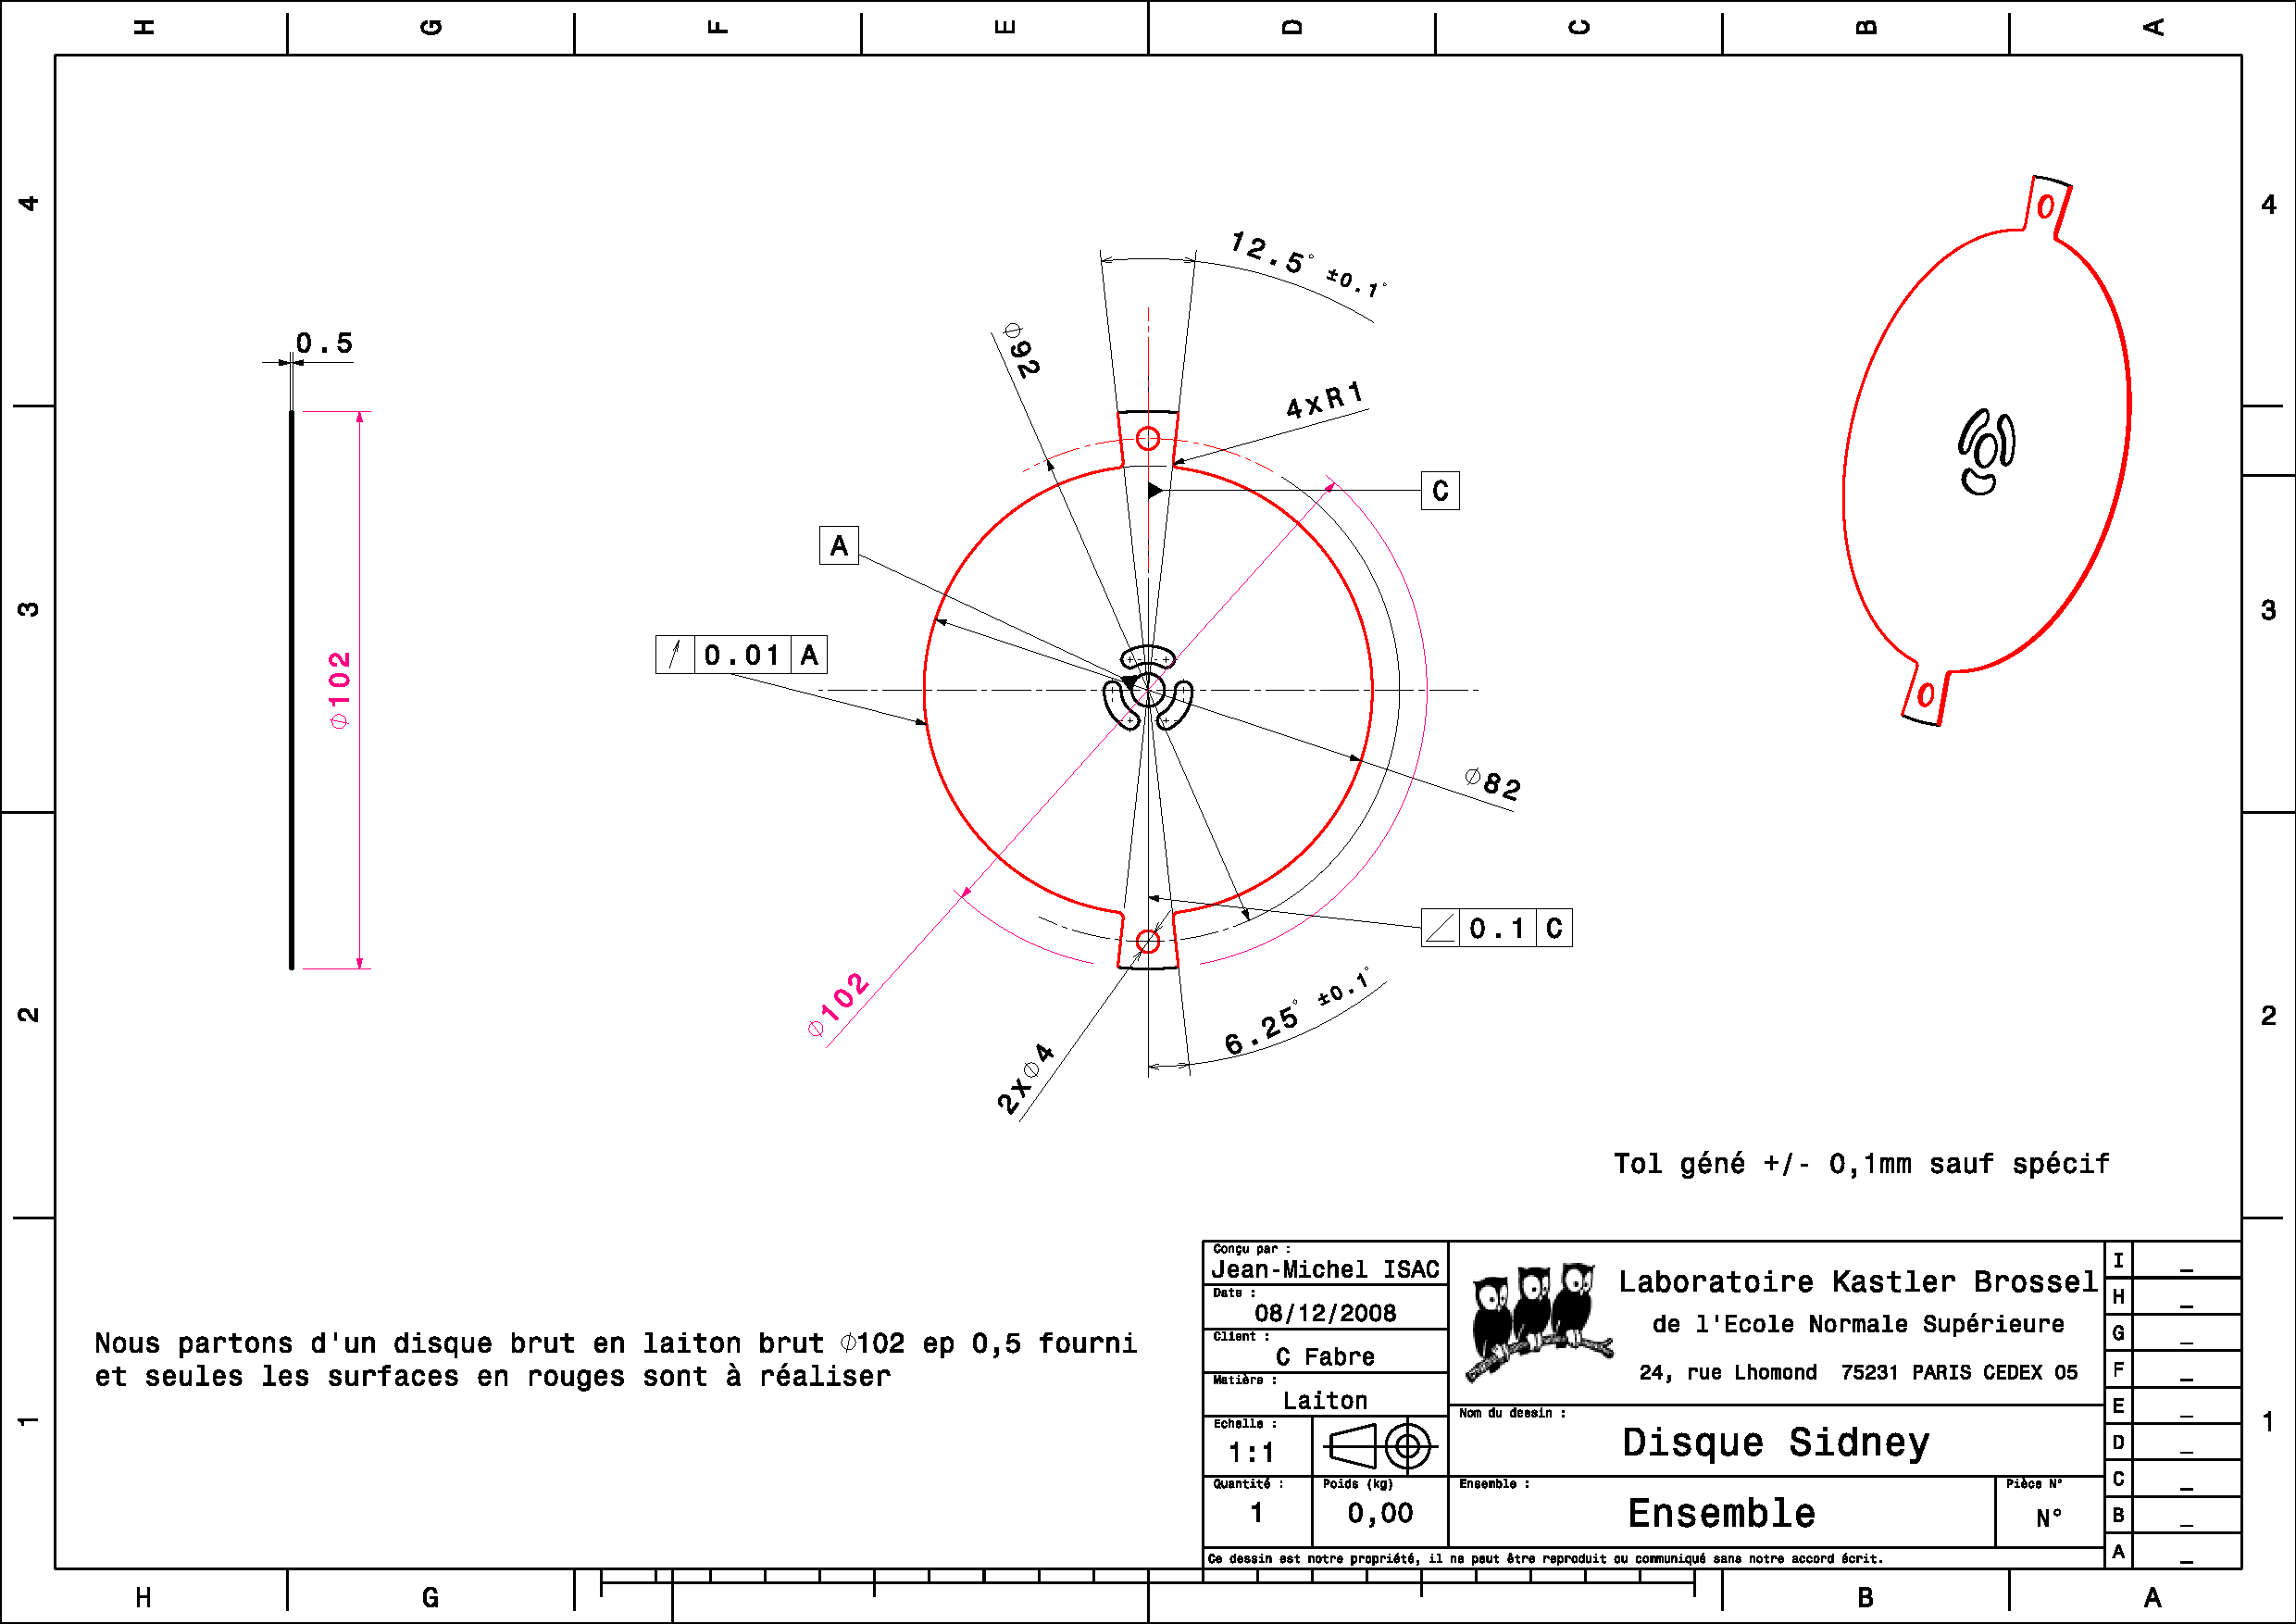
\includegraphics[width=0.45\textwidth]{figures/chopper} 
 \caption[Scitec 310CD Chopper]{Scitec 310CD chopper with protective case opened to show optical fork.} 
 \label{fig:chopper_open} 
\end{figure}


\subsubsection{Rotating Disc}
\label{rotating_disc} 

We then sought to mount the slits onto the discs provided.  For the memory experiment, we wanted the light to follow a particular on/off sequence.  During a long period A, we wanted the squeezed beam to pass into the atoms, which would allow us to track the relative phase between the squeezed beam and the local oscillator.  Then for a shorter period B, we wanted to cut off the squeezing creating a \emph{dark time} in order to finalize the preparation of the MOT.  Finally, we would present the actual pulse in C, after which the sequence would relaunch.  Figure \ref{fig:timing_diagram} illustrates this concept.

\begin{figure}[!ht] 
 \centering 
 \includegraphics[width=0.55\textwidth]{figures/timing_diagram} 
 \caption[Optical timing sequence for pulse generation]{Optical squeezed vacuum pattern needed for storing a pulse in the quantum memory.  We track the phase at A (25 ms), prepare the memory at B (100 $\mu s$), and store the pulse at C (1 $\mu s$).} 
 \label{fig:timing_diagram} 
\end{figure}

Our proposed solution to create this sequence was to construct a slotted disc with protruding teeth.  By placing the Thorlabs slit into the disc, the light could pass by the disc for the majority of the time, be blocked by the protruding tooth, and reappear when aligned with the tiny slit, producing the pulse.  


\subsubsection{Disc Balancing}
\label{disc_balancing} 

As the disc was rotating at 200 rps, the slightest imbalance could introduce instabilities into its rotation, and thus create jitter.  Thus, we constructed a symmetric disc having protrusions on both sides in order to maintain the balance.  

Introducing a second slit to the disc preserves its balance, however because no two slits are exactly identical, the size of the pulse created from the second slit has no relation to the first, which means that we can't use both pulses for the experiment.  The simplest solution that we developed was to just ignore the TTL produced from the second slit, so that it would not trigger the experiment.  In Chapter \ref{ch:7}, we will discuss the FPGA techniques used to create a TTL decimator, which allowed us to selectively ignore certain signals.  As we only used one of the slits, we placed a 200 $\mu m$ slit into the second side in order to have a more versatile disc for experimenting with different pulse sizes.


\subsubsection{Disc Geometry}
\label{disc_geometry} 

We determined that the slit needed to be placed at a 46 mm radius from the disc center, and that the tooth needed to cover an angle of 12.45\textdegree .  This would allow us to produce pulses of around 1 $\mu s$, and dark periods of around 100 $\mu s$ for a 4 ms rotation period at 200 rps.  We had the disc cut from our design shown in Appendix \ref{appendix:chopper_disc_diagram} by a commercial agency, and the end result produced the disc shown in Figure \ref{fig:chopper_disc}.

\begin{figure}[!ht] 
 \centering 
 \includegraphics[width=0.30\textwidth]{figures/chopper_disc} 
 \caption[Custom designed disc for optical chopper]{Customized disc designed to hold both 200 $\mu m$ and 50 $\mu m$ Thorlabs slits.} 
 \label{fig:chopper_disc} 
\end{figure}


\subsubsection{Pulse Measurements}
\label{pulse_measurements} 

We then mounted the chopper assembly and securely fastened it to the table, and locked the OPO with a seed beam injected so that we could directly observe the pulses produced on the squeezed light path.  As the chopper's rotation speed and stability exceeded our initial estimated requirements, we managed to produce well-formed pulses with widths down to 450 ns.  Furthermore, by comparing the pulse amplitude to the amplitude of the light not passing through the slit, such as in Figure \ref{fig:200um}, we can see that our tight focusing allowed us to avoid any diffraction losses. The pulses shown in Figure \ref{fig:chopper_pulses} illustrate our results.
  
\clearpage
\begin{figure}[!ht]
  \centering
  \subfloat[][3 $\mu s$ ]{
    \label{fig:3us}
    \includegraphics[width=0.41\textwidth]{figures/chopperzoom50100} }
  \subfloat[][1.5 $\mu s$ ]{
    \label{fig:1.5us}
    \includegraphics[width=0.41\textwidth]{figures/chopperzoom50200} } \\
  \vspace{-10pt}
  \subfloat[][1.0 $\mu s$ ]{
    \label{fig:1us}
    \includegraphics[width=0.41\textwidth]{figures/chopperzoom50300} }
  \subfloat[][780 ns]{
    \label{fig:780ns}
    \includegraphics[width=0.41\textwidth]{figures/chopperzoom50400} } \\
  \vspace{-10pt}
  \subfloat[][640 ns]{
    \label{fig:640ns}
    \includegraphics[width=0.41\textwidth]{figures/chopper50500} } 
  \subfloat[][520 ns ]{
    \label{fig:520ns}
    \includegraphics[width=0.41\textwidth]{figures/chopperzoom50600} } \\
  \vspace{-10pt}
  \subfloat[][450 ns]{
    \label{fig:450ns}
    \includegraphics[width=0.41\textwidth]{figures/chopper50700} } 
  \subfloat[][1.6 $\mu s$ - shortest pulse created with 200 $\mu m$ slit]{
    \label{fig:200um}
    \includegraphics[width=0.41\textwidth]{figures/chopper200800side} }
  \caption[Optical chopper pulse measurements]{Optical pulses created using the 50 slits $\mu m$ \subref{fig:3us} - \subref{fig:450ns} and 200 $\mu m$ slits \subref{fig:200um} }
  \label{fig:chopper_pulses}
\end{figure}

\clearpage

Thus, the chopper did manage to create the stable short pulses that we required, however there were a few critical drawbacks.
\subsubsection{Noise}

Due to the chopper's high rate of speed, it created a large amount of noise which filled the entire room, disrupting other sections of the experiment.  We tried to minimize this noise by using smaller holes to inject the light into the chopper, and we installed the entire apparatus in the plexiglass box shown in Figure \ref{fig:chopper_box} that was lined with lead and foam.  This completely removed the noise at rotational speeds up to 600 Hz.

\begin{figure}[ht] 
 \centering 
 \includegraphics[width=0.45\textwidth]{figures/chopper_box} 
 \caption[Acoustic isolation box for dampening chopper noise]{Plexiglass box used to attenuate the acoustic noise from the chopper.  The interior of the box was coated with a foam/lead material to absorb the sound.  Silent performance up to 600 Hz.} 
 \label{fig:chopper_box} 
\end{figure}

 
\subsubsection{Vibrations}
\label{vibrations} 

A more critical problem however, arose from the vibrations transmitted from the chopper to the table.  This would be expected since the chopper was securely fastened to the table, however as a result, these vibrations prevented us from maintaining the OPO locked at resonance.  We thus attempted to attenuate the vibrations by placing a sandwich of isolating material underneath the chopper as shown in Figure \ref{fig:chopper_sandwich}.  Through trial and error, we chose a mixture of aluminum, lead, styrofoam and sorbothane, as well as placed sheets of lead beneath the OPO itself for increased attenuation.


\begin{figure}[!hbt] 
 \centering 
 \includegraphics[width=0.45\textwidth]{figures/chopper_sandwich} 
 \caption[Chopper vibration isolation stack]{Isolation sandwich used to attenuate chopper vibrations, consisting of aluminum, lead, styrofoam, and sorbothane.} 
 \label{fig:chopper_sandwich}  
\end{figure}
   
\subsubsection{Jitter}
\label{jitter} 

When using the chopper, the entire experiment needed to be triggered from the chopper pulse because the exact time when the pulse would be created was uncertain.  This posed a problem because as stated earlier, EIT storage required us to have a 100 ns predictability of the pulse arrival time.  Despite our successes in removing the acoustic noise and attenuating the chopper vibrations, problems of pulse jitter re-arose and proved to be a final problem.  When we fixed the chopper rigidly to the table, the jitter was on the order of several ns.  However, when we used the isolation to attenuate the mechanical vibrations, we could no longer securely fasten the chopper to the table, and thus its movement created pulse jitter of 500 ns.  This uncertainty was much too large for us to properly use the EIT protocol, and it made it impossible for us to predict to within 100 ns when the next pulse would arrive - thus ruining the timing for the pulse detection and triggering the experiment.  



%% \subsection{Quantum Tomography of Pulsed Squeezing} 
%% TODO


%% \bookmarksetup{startatroot}
\chapter*{Publication}
\addstarredchapter{Publication}
\markboth{Publication}{}
\label{article} 

\thispagestyle{empty}

\resizebox{!}{0.05mm}{.}

\vspace{6em}

\paragraph{Reproduction of article published in Optics Express:}
\ \vspace{5.4ex}
\\
\indent

S. Burks, J. Ortalo, A. Chiummo, X. Jia, F. Villa, A. Bramati, J. Laurat, and E. Giacobino, "Vacuum squeezed light for atomic memories at the $D_2$ cesium line," Opt. Express  17, 3777-3781 (2009).


\cleardoublepage

%% \includepdf[pages={1-4}]{opex.pdf} 


\addtolength{\hoffset}{-1.2in}
\thispagestyle{empty}
\begin{figure}[!ht]
  \vspace{-3.5cm}
  $$
  \epsfig{file=opex_1,width=1.40\textwidth}
  $$
\end{figure}
\clearpage
  
\thispagestyle{empty}
\begin{figure}[!ht]
  \vspace{-3.5cm}
  $$
  \epsfig{file=opex_2,width=1.40\textwidth}
  $$
\end{figure}
\clearpage
  
\thispagestyle{empty}
\begin{figure}[!ht]
  \vspace{-3.5cm}
  $$
  \epsfig{file=opex_3,width=1.40\textwidth}
  $$
\end{figure}
\clearpage
  
\thispagestyle{empty}
\begin{figure}[!ht]
  \vspace{-3.5cm}
  $$
  \epsfig{file=opex_4,width=1.40\textwidth}
  $$
\end{figure}
\clearpage
   
\addtolength{\hoffset}{1.2in}



\part{Preparation of a Quantum Memory With Cold Atoms}
\label{part:3} 
\chapter{Experimental Tools for the Storage of Squeezed Light}
\minitoc

 
\section{Introduction}

Over the last several years, our group has focused on the development of a quantum memory in Cesium.  The idea is based on using EIT to carry out a reversible transfer of the quantum fluctuations of light onto the transverse spin components of an ensemble of Cesium atoms.  The theory describing this approach was developed during the thesis of Aurelien Dantan \cite{DantanPhD}.  During the work carried out afterwards by Jean Cviklinski \cite{CviklinskiPhD} and Jeremie Ortalo \cite{ortalo}, a memory was developed using warm Cesium vapor where the Zeeman sublevels served as the fundamental levels for EIT.  This work resulted in showing that we could carry out a noiseless storage and retrieval of coherent states.  As the Zeeman sublevels are closely spaced in frequency, we have focused our next memory implementation on using the hyperfine transitions for EIT, which will allow us a much finer frequential resolution for the signal and control transitions.

In this chapter, we will discuss our development of this new implementation of
a quantum memory, and describe the experimental elements needed to store
squeezed light onto a cold Cesium vapor.  Our main goal for this
implementation of the memory is to show that we can achieve the storage and
retrieval of squeezed vacuum states using the cold atomic medium.  Once we
accomplish this, we can create entangled beams from our squeezed vacuum, and
store these entangled states into separate regions of our ensemble.
Accomplishing this goal will show that it is possible to create a quantum memory which can function as the core component in a quantum repeater network. 

As this work takes a departure from our previous experimental approaches, it requires us to develop new tools and techniques before we will have system that is usable for storage.  In the following sections, we will discuss the individual components that were assembled in order to advance our progress towards a working quantum memory.

\subsection{Optical Storage Through EIT} 

As stated earlier, the storage mechanism that we will use for this experiment is
EIT \cite{harris1997electromagnetically}.  For this method, we use the 3-level
$\Lambda$ system shown in Figure \ref{fig:eit_transitions}, where the
fundamental levels are the F=3 and F=4 hyperfine states, and the excited level
is the F'=4 state.  Our atoms will be initially prepared by pumping them into
the F=4 state.  We will then use the F=3 $\to$ F'=4 transition for our control
beam to dress the F'=4 level.  We then tune our signal pulse on the F=4 $\to$
F'=4 transition, ans as it is not resonant with the dressed F'=4 level, this
leads to a transparency for our signal.  Once the signal pulse has entered the atomic ensemble, we extinguish the control beam to trap the signal pulse for a small time period, which is the memory storage time.  We then reactive the control beam to release the signal pulse, and read the stored state from the memory.

\begin{figure}[!ht] 
 \centering 
 \includegraphics[width=0.35\textwidth]{figures/eit_transitions} 
 \caption[EIT transitions for Cesium quantum memory]{Transitions used to carry out EIT in Cesium for the quantum memory.  The F=3 and F=4 hyperfine levels serve as the ground states, with an F'=4 excited state.  A control beam F=3 $\to$ F'=4 controls the transparency of the atomic ensemble, while a signal is encoded onto the F=4 $\to$ F'=4 beam.} 
 \label{fig:eit_transitions} 
\end{figure}
 

\section{Phase Lock}

When carrying out experiments with atoms involving atomic coherence effects, it is necessary that the lasers used to probe the atomic transitions possess a narrow linewidth and a high optical coherence with each other \cite{hockel2009robust}.  Specifically with EIT, changes in the laser linewidth can affect the EIT transparency and our ability to slow down and store light \cite{lu2008realization}.

Typically when performing EIT, if we are studying the coherence effects between transitions having a small frequency difference, such as the Zeeman sublevels, the frequency range is small enough to allow us to probe the levels using one main source laser.  We can accomplish this by passing a fraction of the laser through an AOM or EOM, and thus create a second frequency shifted beam on output.  This shifted beam will have the highest possible degree of coherence with the original beam, as they both originate from the same laser source.

For probing the hyperfine levels of Cesium however, the 9.2 GHz frequency separation is far too large to achieve efficiently using an AOM.  Large band EOMs are
available, but their high costs and low efficiencies prevent us from using this
option to directly create an intense frequency shifted beam.

For this case, it is simpler to use two separate lasers to explore the two transitions.  For our experiment, we decided to tune the Matisse laser to the F=4 $\to$ F'=4 signal transition, and use a separate diode slave laser for the F=3 $\to$ F'=4 control beam.  In order to preserve the coherence between the two lasers, we need to develop a way to lock them in phase such that the relative change of phase between the master laser and the slave laser rests locked at a fixed beat frequency.  To accomplish this phase lock, we have developed an Optical Phase Locked Loop (OPLL) as a feedback system to lock the diode laser to the Matisse.

\subsection{Theory} 
 
In order to understand how the OPLL functions, we can begin by analyzing the
simpler electronic PLL on which it is based \cite{curtin1999phase3}.  We begin
by sending our PLL a signal frequency from a voltage-controlled oscillator
(VCO), and a reference frequency to which we wish to lock the VCO and reduce its linewidth.  We take these two signals and compare them using a phase-frequency detector (PFD), which outputs an error signal based on their phase and frequency difference.  We then filter this error signal using a low-pass loop filter, which must be properly tuned to the system \cite{abramovitch2002phase}, and we use the output from this filter as feedback to control the VCO frequency.  We can optionally pass the VCO feedback through a frequency divider if we need to run the VCO at a much higher rate than the reference frequency.  When the circuit is activated, the VCO locks its frequency to the reference frequency at a reduced linewidth.  The block diagram in Figure \ref{fig:pll_block}  illustrates this operation.

\begin{figure}[!htb] 
 \centering 
 \includegraphics[width=0.75\textwidth]{figures/pll_block} 
 \caption[PLL block diagram]{A typical PLL is composed of a phase-frequency detector (PFD), low-pass filter (LPF), voltage-controlled oscillator (VCO), and frequency divider (f-DIV).  The VCO signal is fed back into the PFD for comparison to the reference signal} 
 \label{fig:pll_block} 
\end{figure}
 
\begin{eqnarray}
  \label{eq:pll_eq}
  S(t) = A_1 \sin \left(\omega_1 t + \phi_1(t)\right) = A_1 \sin (\Phi_1) \\
  R(t) = A_2 \sin \left(\omega_2 t + \phi_2(t)\right) = A_2 \sin (\Phi_2) 
\end{eqnarray}

\noindent
If we imagine our signal and reference as two periodic signal $S(t)$ and $R(t)$, engaging the phase lock assures a fixed relationship between our signal arguments, such that 

\begin{equation}
  \label{eq:pll_def}
  \Phi_1=\Phi_2.
\end{equation}

\noindent
Given this description of a PLL, there are two core components which must be properly adjusted in order to optimize the system - the phase-frequency detector, and the loop filter.


\subsubsection{Frequency Division}

The PLL response is limited to its reference signal's input frequency, but often we wish to run a VCO at a much higher frequency.  We can accomplish this by adding a frequency divider to the VCO output.  By dividing the VCO signal frequency to a lower value closer to the reference frequency, we can compare the reference and signal frequencies without artificially slowing down our VCO.  

Additionally, we can consider this division as a type of \emph{gain} on our PLL control signal.  By dividing the VCO output by $n$, the PLL can use the same voltage to correct for a range of $n$ times the reference frequency, as opposed to only correcting for a range around the reference frequency without a divider.  This can potentially increase the loop performance by allowing us to use small control signal voltages for a large response.



\subsubsection{Phase-Frequency Detection}

There are several methods of creating phase detector for signal comparison.  For our design, we use an all-digital PFD.  This system is composed of a set of digital flip-flops which execute the logic shown in Figure \ref{fig:pfd_logic} \cite{mch12140}.

\begin{figure}[!ht] 
 \centering 
 \includegraphics[width=0.55\textwidth]{figures/pfd_logic} 
 \caption[Phase-frequency detector logic diagram]{Logic diagram for the all-digital phase-frequency detector used in our PLL.  Phase and frequency changes in the reference (R) and signal (V) inputs cause digital state changes on the U, $\bar{U}$, D, and $\bar{D}$ outputs, allowing us to create an error signal.} 
 \label{fig:pfd_logic} 
\end{figure}

A digital PFD takes a reference (R) and VCO (V) signal as input, and outputs four signals based on their phase or frequency difference.  By subtracting either the positive (U-D) or negative ($\bar{U}$-$\bar{D}$) signals, we can receive an error signal on the output, as is shown in Figure \ref{fig:pfd_output} \cite{mch12140}.  The error signal output from the PFD is proportional to the frequency and phase error of our input. 

\begin{figure}[!ht] 
 \centering 
 \includegraphics[width=0.55\textwidth]{figures/pfd_output} 
 \caption[PFD output signal]{Output voltage as a function of phase $\Phi$ from a PFD after subtracting the $U-D$, or $\bar{U}-\bar{D}$ outputs.} 
 \label{fig:pfd_output} 
\end{figure}




\subsection{Experimental Setup} 

\begin{figure}[!ht] 
 \centering  
 \includegraphics[width=0.55\textwidth]{figures/pll_table} 
 \caption[OPLL optical table photo]{Photo of optical table used for the OPLL.} 
 \label{fig:pll_table} 
\end{figure}


Creating an Optical PLL follows the exact same procedure as a traditional PLL.  Instead of using a VCO, we use the beat signal generated from the optical interference of our slave and master lasers, and we use the filtered error signal to adjust the frequency tuning of the slave laser.  We have three main methods to adjust the frequency of a slave laser:  changing the cavity length, changing the diode temperature, or modulating the injection current.  The current
 modulation approach has the fastest response and allows for the largest loop bandwidth, so we use this approach.

  

\begin{figure}[!ht]
  \centering
  \subfloat[][OPLL optical block diagram.  A few mW of light from the Matisse and Diode are mixed onto a photodetector.  90\% of the diode light continues to a saturated-absorption cell, and the MOT.]{
    \label{fig:pll_block_optical}
    \includegraphics[width=0.5\textwidth]{figures/pll_block_optical} }
  \subfloat[][OPLL Electronic block diagram.  A biased photodiode detects a 9.0 GHz optical beat signal, which is then amplified +30dB and mixed down to 400 MHz.  The beat signal enters the PLL along with a 100 MHz reference to create the error signal, which is then integrated, and used to control the diode modulation.]{
    \label{fig:pll_block_electronic}
    \includegraphics[width=0.5\textwidth]{figures/pll_block_electronic} } \\
  \caption[OPLL block diagrams]{Optical and electronic block diagrams for our OPLL implementation }
  \label{fig:opll_block}
\end{figure}

Figure \ref{fig:pll_block_optical} shows the optical layout of our
phase-locking system pictured in Figure \ref{fig:pll_table}.  Our setup begins
with us creating a beat signal from the interference of the Matisse and diode
lasers.  To accomplish this, we combine a few mW of light from the Matisse
with an equal amount of light from the diode on a non-polarizing beam splitter. The two light sources are aligned to have the same matching and polarization.  We then send the light into a Hamamatsu photodiode which is powered by a 9V battery, and biased with a Minicircuits ZX85-12G-S+ Bias Tee with a 12 GHz bandwidth.  The usage of a battery allows us to minimize the electronic noise in the photodiode.

Next, we lock the Matisse to the 4-4 transition, and manually adjust the diode
laser so that it is near the 3-4 transition, and separated by approximately
9.0 GHz.  We lock at 9.0 GHz instead of 9.2 GHz because we pass our diode
laser through an AOM before sending it on to the MOT.  The AOM adds the
remaining 200 MHz offset we need to reach 9.2 GHz, and allows us to easily
create pulses of this light.  

The optical interference of the two lasers
creates a beat note which is detected by the biased photodiode, as shown in
Figure \ref{fig:pll_block_electronic}.  By adjusting the
optical power, we amplify the beat note power up to around 0 dBm.  We then send the photodiode output to an Amplical AMP8G12-33 amplifier where
it is amplified by 30 dB and then sent to a Minicircuits ZMX-10G+ mixer.  We
demodulate the note with a microwave 8.6 GHz signal generated by a HP 8672A signal generator.  This allows us to mix down the optical beat note to 400 MHz, allowing us to observe it on our low-frequency spectrum analyzer as shown in Figure \ref{fig:beat_note}.  This is convenient because we can from this point on, avoid using high-frequency RF components in our electronics chain, and use a simpler low-frequency setup.  

\begin{figure}[!ht] 
 \centering 
 \includegraphics[width=0.55\textwidth]{figures/beat_note} 
 \caption[Optical PLL beat note demodulated to 400 MHz]{Optical beat note between Matisse and diode lasers demodulated to 400 MHz.} 
 \label{fig:beat_note}
\end{figure}

Once we have the 400 MHz beat note, we use a Minicircuits ZFDC-10-2
directional coupler to extract 10\% of the signal and send it to a spectrum
analyzer which permits observation of the lock. The remaining 90\% continues
on to two ZFL-500LN-BNC amplifiers, which give a total amplification of 10 dB,
and then on to a homemade wideband 0-400 MHz preamplifier circuit which
amplifies the signal by up to an additional 20 dB.  We then send the beat note to our
phase-frequency detection circuit, which creates the error and modulation
signal that we then use to lock the diode.  The last step in our chain
involves passing the modulation signal through the integrating circuit shown
in Figure \ref{fig:pll_integrator}, which acts as our loop filter.  We then send this integrated output directly into the current modulation input for the diode laser.


\begin{figure}[!ht] 
 \centering 
 \includegraphics[width=0.55\textwidth]{figures/pll_circuit_block} 
 \caption[PLL circuit block diagram]{Block diagram showing our PLL functionality.  The 400 MHz signal is divided by 4, and compared to a 100 MHz reference with the PFD.  A differential op-amp subtracts the PFD outputs to create the error signal.} 
 \label{fig:pll_circuit_block} 
\end{figure}

\begin{figure}[!ht] 
 \centering 
 \includegraphics[width=0.55\textwidth]{figures/pll_whole} 
 \caption[PLL circuit photo]{Photo of actual OPLL circuit with notable features marked.} 
 \label{fig:pll_whole} 
\end{figure}

 
Figure \ref{fig:pll_circuit_block} depicts the operation of our PLL circuit pictured in Figure \ref{fig:pll_whole}.  For our reference signal, we use a 100 MHz signal generated by an Agilent 
E4420b generator.  Our 400 MHz beat note enters the PLL circuit where it is
divided by 4 using an ON Semiconductor MC12093 divider, and the divided signal
and our reference are compared using an ON Semiconductor MCH12140 PFD.  The
PFD outputs signals on its U and D outputs which we then subtract using a
differential operational amplifier (opamp).  The opamp then outputs the error signal, which we send
directly to the integrator circuit for low-pass filtering.

In order to interface the filtered modulation signal with the laser diode, we
use the current divider circuit shown in Figure \ref{fig:bias_t} to limit the
current applied by our PLL circuit.  This allows us to avoid destroying the
laser by applying too much modulation current.


\begin{figure}[!ht]
  \centering
  \subfloat[][PLL integrator circuit.]{
    \label{fig:pll_integrator}
    \includegraphics[width=0.65\textwidth]{figures/pll_integrator} }
  \subfloat[][Diode current modulation interface.]{
    \label{fig:bias_t}
    \includegraphics[width=0.35\textwidth]{figures/bias_t} } \\
   \caption[OPLL integrator and diode current modulation circuits]{\subref{fig:pll_integrator} Circuit Diagram for PLL Integrator  \subref{fig:bias_t} Current modulation circuit to interface PLL with diode laser.  The current divider protects the diode from too much modulation current.}
  \label{fig:opll_circuits}
\end{figure}
    

Using this setup, once we tune the diode laser to place the beat signal near the reference frequency, we can observe the error signal take the form in Figure \ref{fig:pll_err}, which resembles the logic diagram output in Figure \ref{fig:pfd_output}.


\begin{figure}[!ht]
  \centering
  \subfloat[][OPLL error signal as the beat signal approaches the lock point.  We see that this resembles the output shown in Figure \ref{fig:pfd_output}.]{
    \label{fig:pll_err}
    \includegraphics[width=0.5\textwidth]{figures/pll_err} }
  \subfloat[][Error signal goes to zero when we engage the OPLL lock.]{
    \label{fig:pll_locked}
    \includegraphics[width=0.5\textwidth]{figures/pll_locked} } \\
  \caption[OPLL error signal]{PLL error signal as we a) approach the lock point and b) engage the lock.}
  \label{fig:pll_error}
\end{figure}


At this point when we engage the phase lock, the slave laser locks to the
Matisse and the optical beat note produces the noise
trace shown in Figure \ref{fig:phase_lock_results}.


%% \begin{figure}[ht] 
%%  \centering 
%%  \includegraphics[width=0.70\textwidth]{figures/phase_lock} 
%%  \caption[Phase lock scan]{Diode laser phase-locked to the Matisse at a 9.2Ghz shift.  The majority of the power is held within the central peak.} 
%%  \label{fig:phase_lock_results} 
%% \end{figure}


\begin{figure}[!ht]
  \centering
  \subfloat[][Diode laser phase-locked to the Matisse at a 9.0 GHz frequency
  offset.  The majority of the power is held within the central peak.  This
  system maintains a lock for over 10 hours, and is only sensitive to the slow
  long-term stability drifts.]{
    \label{fig:phase_lock_bbig}
    \includegraphics[width=0.5\textwidth]{figures/phase_lock} }
  \subfloat[][Zoom of central peak with 10 Hz span, 1 Hz VBW and RBW.  This zoom
  shows that our system maintains a frequency lock with a precision of better
  than 1 Hz.  Our resolution of the ultimate lock precision is limited by the spectrum
  analyzer.]{
    \label{fig:pll_1hz}
    \includegraphics[width=0.5\textwidth]{figures/pll_1hz} } \\
  \caption[Phase lock results]{ Phase lock results}
  \label{fig:phase_lock_results}
\end{figure}


\subsection{Analysis} 

In order to quantify the quality of the phase lock, we can use the mean-square error of the phase noise.  This quantity is defined as the ratio of power in our beat signal at its center frequency, and the power integrated over all frequencies.  We take the center frequency power as simply the height of our central peak given by the spectral analyzer.  

We can derive this quantity by defining the noise density as was done earlier for the electric field, and as is seen in \cite{zhu1993stabilization}.  We begin by defining the E field of our laser as 

\begin{equation}
  \label{eq:pll_e}
  E(t) = A(t)e^{-i \omega_0 t - i \phi t},
\end{equation}

\noindent
where A(t) is the instantaneous field amplitude, and $\phi(t)$ is the phase modulation.  We have an instantaneous angular frequency given by 

\begin{equation}
  \label{eq:pll_om}
  \omega (t) = \omega_0 + \d{\phi(t)}{t}.
\end{equation}

\noindent
We can write the autocorrelation function of our field as 

\begin{equation}
  \label{eq:pll_ac}
  R_\epsilon (\tau) \equiv \avg{E(t)E^*(t+ \tau)},
\end{equation}

\noindent
and by taking the Fourier transform, we can obtain

\begin{equation}
  \label{eq:pll_pow}
  P_\epsilon(\tau) = \frac{1}{2\pi} \intind P_\epsilon (\omega ) d \omega  
\end{equation}

\noindent
We can find the mean square noise error by measuring the fraction of the power contained at our lock frequency with respect to the total power

\begin{equation}
  \label{eq:pll_rms}
  exp(-\avg{\Delta \phi^2}) = \frac{P_0}{\intind P(\omega ) d \omega } 
\end{equation}

\noindent
\req{eq:pll_rms} allows us to establish a quantitative measure of the phase
noise contained in the lock by using a spectrum analyzer to measure the power contained in the peak, and
the total integrated power \cite{appel2009versatile}.
%% \noindent
%% Using \req{eq:pll_rms}, we obtain a phase noise for our lock of XXXXXXXX???????



\section{The Magneto-Optical Trap}

The principle component of this experiment is the MOT itself which contains
our trapped atoms.  We will begin by describing the characteristics of the
MOT, and the experimental elements that allow us to prepare a dense atomic
cloud inside of it.

\subsection{Basic Trapping Principles} 

In order to trap our atoms inside the MOT, we need to create a system for
cooling and confining the atoms in a small region.  We first require three
pairs of counter-propagating beams, where one pair of beams is aligned with each
spatial axis.  The beams are circularly polarized such that two pairs take a
$\sigma^+$ polarization, and one pair takes a $\sigma^-$ polarization. These
trapping beams are detuned from the F=4 $\to$ F'=5 Cesium cycling transition by
10 MHz.  This detuning from resonance allows us to the Doppler effect to apply a velocity-dependant breaking force to the atoms, and thus create an optical molasses at the point where the beams meet at the center of the MOT.


%% \begin{figure}[!ht] 
%%  \centering 
%%  \includegraphics[width=0.35\textwidth]{figures/mot_transitions} 
%%  \caption[MOT trapping and repumping beam transitions]{} 
%%  \label{fig:mot_transitions} 
%% \end{figure}


\begin{figure}[!ht]
  \centering
  \subfloat[][We require three circularly polarized beams to create the optical molasses, and a magnetic field gradient to confine the atoms.  A repump beam is superposed with the trapping beam along two axes.]{
    \label{fig:mot_ill}
    \includegraphics[width=0.5\textwidth]{figures/mot_ill} }
  \subfloat[][Optical transitions used for the trapping and repumping beams in the MOT.  The trapping beam is detuned by 10 MHz from the F=4 $\to$ F'=5 transition.  The repumping beam is resonant with the F=3 $\to$ F'=4 transition.]{
    \label{fig:mot_transitions}
    \includegraphics[width=0.5\textwidth]{figures/mot_transitions} } \\
   \caption[MOT illustration and transitions]{Requirements for building a MOT.   Converging beams and magnetic field gradients trap the atoms when we use the F=4 $\to$ F'=5 trapping transition.}
   \label{fig:mot_ill_trans}
\end{figure}

As some of the atoms relax into the F=3 state, we also require a repump beam for the F=3 $\to$ F'=4 transition, so that we can repump these atoms into the F=4 state allowing us to retrap them.  We overlap two of these repump beams with two of the trapping beams described earlier. Figure \ref{fig:mot_transitions} depicts the 3-level diagram that shows the relevant transitions needed for creating the molasses.   


Once the optical molasses is created, we also need to apply a magnetic field gradient so that we can confine the atoms to a small region.  We supply the MOT chamber with the necessary beams via fiber optic, which prevents the beams from disaligning on a day-to-day basis.

In the following sections, we discuss the experimental setup that we developed in order to fulfill these requirements and create our atomic ensemble.

\subsection{MOT Characteristics} 

For the trap itself, we selected a glass chamber with 7 viewports on its
sides, as shown in Figure \ref{fig:mot_glass}.  This allows us a large flexibility in how we inject our beams into the
chamber.  We inject the trapping beams through the opposing windows to create
an optical molasses in the chamber center.  In order to create the magnetic field, we wound 120 loops of copper wire into coils around circular Teflon frames, which had a radius of 10 cm.  The coils were positioned at each side of the trap and fixed to the table with brass posts.  Brass was selected for the post material as it does not respond to magnetic fields.  We typically sent 5A of current into the coils to create the fields.  The chamber's glass composition also aids with respect to the magnetic field as it prevents the creation of Foucault currents when we cut off the field.

\begin{figure}[!ht]
  \centering
  \subfloat[][Glass chamber used to create the MOT with multiple input ports.]{
    \label{fig:mot_glass}
    \includegraphics[width=0.5\textwidth]{figures/chamber} }
  \subfloat[][Atoms trapped at the center of the chamber]{
    \label{fig:chamber_mot}
    \includegraphics[width=0.5\textwidth]{figures/atoms_mot} } \\
   \caption[Glass MOT chamber]{MOT Chamber used to trap the atomic ensemble.} 
  \label{fig:mot_chamber}
\end{figure}

We create an initial vacuum in the chamber by pumping the pressure down to $10^{-7}$ torr.  At this point, we activate an ion pump which further decreases the pressure to $10^{-9}$ torr or lower.  

Cesium atoms are injected into the chamber by means of a set of getters, which are Cesium filled wires that were installed inside of the chamber during its construction.  When we pass a strong current through these getters, they heat up to around $400^\circ C$, and begin to release their Cesium.  We typically send around 5A of current through the getters, which yields the largest MOT with the highest density of atoms.  Using this configuration, we have managed to trap an estimated $10^9$ atoms.  

\subsection{Laser Sources} 
  
To create the beams at all of the necessary transitions, we developed a set of diode lasers and used them along with a Toptica Photonics BoosTA Master Oscillator Power Amplifier (MOPA) to produce a high optical output for our trapping beam.  The diodes used to create the laser transitions were constructed from designs
developed at the Paris Observatory \cite{Baillard06}.  Figure
\ref{fig:ioe_labeled} shows an example of one of the diodes.  Their bodies consist of a monolithic aluminum alloy, inside of which we fix two mirrors to create a linear cavity.  An interferential filter placed between the mirrors serves as the frequency selecting element, and has a transmissivity of 90\% and a FWHM of 3 nm.  The output mirror of the cavity has a transmissivity of 30\% and is mounted to a piezo which controls the cavity length.


\begin{figure}[!ht]
  \centering
  \subfloat[][Simplified illustration of diode components.]{
    \label{fig:diode_block}
    \includegraphics[width=0.41\textwidth]{figures/diode_laser_block} }
  \subfloat[][Photo of diode with open casing, and actual components identified. ]{
    \label{fig:ioe_labeled}  
    \includegraphics[width=0.41\textwidth]{figures/diode_labeled} } \\
  \caption[Laser diode]{Laser diode constructed from models developed at the Paris Observatory.}
  \label{fig:diode_lucy}
\end{figure}

 
This design offers several benefits in comparison to the Littrow design that we previously used for our other diodes \cite{ortalo}.  First, the frequency selecting element and the cavity mirrors are decoupled, which grants us the possibility to tune the cavity frequency while independently optimizing it for stability.  The usage of a linear cavity also allows us to change the wavelength by rotating the interferential filter, without changing the direction of the output beam.  Finally, the output mirror is placed in a \emph{cat's eye} configuration, in which the mirror is located in the focal plane of the focusing lens.  This allows us to preserve the cavity stability by nullifying the effects of any changes in the cavity beam direction.

With each of these lasers, we manage to obtain roughly 40 mW of output power at 852 nm.  Initially, the output beams have a highly elliptical shape, thus we use a set of anamorphic prisms with a 3:1 ratio to render them Gaussian and usable for the rest of the experiment.

We use two of these diodes to trap the atoms in the MOT and repump them into the
F=4 state.  The diode ``Shaddok'' produces a beam which
is tuned to the 3-4 transition, which pumps the atoms from F=3 to F=4.  We
send this beam into a fibered beam splitter, which provides us with two repump beams at its output near the MOT chamber.  We then apply a circular polarization to these beams and attenuate their output so that they each have around 2 mW of power.  


\begin{figure}[!ht] 
 \centering 
 \includegraphics[width=0.55\textwidth]{figures/diode_setup_block} 
 \caption[Block diagram for diode table]{Trapping and repump beams mix in a fibered beamsplitter to provide 3 trapping beams, and 2 repump beams at the MOT.} 
 \label{fig:diode_setup_block} 
\end{figure}


Next, we use a diode called ``Zeus'' to create the trapping beams for the MOT
which are tuned to the 4-5 transition and red-shifted by 10 MHz.  We use three
trapping beams that enter the MOT chamber from orthogonal directions, and
recombine at its center.  The beams then exit the chamber, where they reflect
off of fixed mirrors and return along their original path, thus trapping the
atoms from 6 directions.  The beams have circular polarizations such that two
of them are left circularly polarized, and the third is right circularly
polarized.  We require around 25 mW of power in each of these three beams.  As
our diode is only capable of producing a total output power of around 40 mW,
we first pass the light through a MOPA which amplifies the power up to 600 mW.
After alignment and coupling losses inside of the MOPA, we have about 300 mW
at the MOPA output that is usable for the experiment.  We then divide this
beam into two segments, sending one segment directly to the MOT chamber, and
sending the other through the second input port of our fibered beam splitter,
as shown in Figure \ref{fig:diode_setup_block}.  
This allows us to obtain a total of three trapping beams at the MOT chamber.





\subsubsection{Locking}
\label{locking} 

In order to lock each diode to its respective transition, we use the saturated
absorption spectroscopy technique to measure the Doppler and
transition peaks.  We then use a lock-in detector to create the error signal
which then passes through to an integrator circuit.  The integrator applies
the feedback control to the piezo mounted in each diode to lock the cavity.
The diodes are also temperature controlled using a homemade controller which
provides us with a temperature regulation having 10 mK stability.  The
frequencies of the diodes are fixed by locking them onto the crossover
resonances which arise due to the closely-spaced excited states.
We then pass each beam through an RF-tuned AOM which allows us to precisely
adjust its frequency.  Table \ref{sat_abs_locks} identifies the crossovers and
AOM frequencies that we use for each laser.  This method allows us to easily adjust the beam around the transition frequency, as well as extinguish it with a digital command.


\begin{table}[ht]
  \centering
  \begin{tabular}{| c | c | c | c |}
    \hline
    Laser & Transition & Lock Point & AOM \\
    \hline
    Repump & F=3 $\to$ F'=4 & 3-4 Crossover  & Order -1: 100 MHz\\
    Trapping & F=4 $\to$ F'=5 -10 MHz  & 4-5 Crossover & Order +1: 115 MHz\\
    \hline
  \end{tabular}
\caption{Transitions and lock points for MOT lasers}
\label{sat_abs_locks}
\end{table}



\begin{figure}[!ht]
  \centering
  \subfloat[][Doppler profile showing the F=4 crossovers and absorption peaks]{
    \label{fig:sas_lucy}
    \includegraphics[width=0.45\textwidth]{figures/lucy} }
  \hspace{-10pts}
  \subfloat[][Doppler profile for the F=3 spectrum.]{
    \label{fig:sas_shadoks}
    \includegraphics[width=0.45\textwidth]{figures/shadoks} } \\
  \caption[Saturated absorption Doppler measurements]{Saturated absorption Doppler measurements of the Cesium F=3 and F=4 lines.}
  \label{fig:sat_abs}
\end{figure}

%% \begin{figure}[!ht] 
%%  \centering 
%%  \includegraphics[width=0.85\textwidth]{figures/Abs_Sat_erreur} 
%%  \caption[Saturated absorption]{Doppler measured using the saturated absorption technique, along with the error signal.} 
%%  \label{fig:label} 
%% \end{figure}

%% \begin{figure}[!ht]
%%   \centering
%%   \subfloat[][caption1]{
%%     \label{fig:label1}
%%     \includegraphics[width=0.5\textwidth]{figures/picture1} }
%%   \subfloat[][caption2]{
%%     \label{fig:label2}
%%     \includegraphics[width=0.5\textwidth]{figures/picture2} } \\
%%    \vspace{-10pt}
%%   \subfloat[][caption1]{
%%     \label{fig:label1}
%%     \includegraphics[width=0.5\textwidth]{figures/picture1} }
%%   \subfloat[][caption2]{
%%     \label{fig:label2}
%%     \includegraphics[width=0.5\textwidth]{figures/picture2} } \\
%%   \caption[Short Caption]{ Long Caption \subref{fig:Short Caption} }
%%   \label{fig:label}
%% \end{figure}

\subsection{Controlling the Magnetic Field} 

While it is necessary to use a magnetic field to create our atomic cloud, the presence of a field during the memory storage can introduce huge limitations to the memory performance.  As the magnetic field in the chamber has an inhomogeneous distribution throughout the atomic cloud, the atoms in different regions of the cloud experience different degrees of Zeeman level splitting.  This results in an inhomogeneous broadening and eventual dephasing of the atoms in different sections of the cloud as the system evolves, finishing with a loss of the collective coherence between the atoms in our ensemble.  When magnetic fields are present, this process can take place within a few hundred nanoseconds \cite{felinto2005control}.  Thus, the decoherence effect fixes an upper limit on the storage time that we can expect with our memory.

By cutting off the magnetic field, we can preserve the coherence between our atoms for a much longer time, and thus expect larger storage times.  Once we begin to cut the magnetic field, the atoms of our cloud immediately begin to disperse.  Thus it is in our interest to cancel out the magnetic field as quickly as possible, so that we can nullify it while maintaining a high atomic density.

In order to control the magnetic field created by the coils, we use a current
driver circuit based on a design published in \cite{garrido2007}.  This design
allows us to control the amount of current flowing through the MOT coils by
applying an analog voltage signal to a control box.  A network of transistors
in the circuit controls the current flowing through to the coils by acting as
a sink, and allows us to create a magnetic field that is proportional to the
applied analog voltage. This circuit is useful in that it not only allows us
to use low control voltages of around 10V, which are easily producible, but we
can also supply it with a relatively low current of 10 A, which is also easily
produced using a commercial generator.  A critical factor to take into
consideration when selecting the circuit components is the choice of the
transistor breakdown voltage.  When we cut off the current flow by setting the
control voltage to 0V, this can create a high voltage back-electromotive force (emf) which can potentially overload and destroy the transistors.  As this emf is determined by the cutoff time, the current flow, and the coil inductances

\begin{equation}
  \label{eq:emf}
  Emf = -L\d{I_L}{t},
\end{equation}
 
\noindent
we have to take these properties into account during our transistor selection.

The details of the circuit construction and characteristics will be described in more detail in the future Ph.D thesis of Lambert Giner.  Here, we focus on describing the optimization of the timing and control mechanism associated with this circuit.


\subsubsection{Control Signal} 

Switching off the magnetic field induces eddy currents in nearby magnetic materials, which can create time and spatially varying magnetic fields around our atoms \cite{garrido2007}.  In order to minimize the effects of these currents, and reduce the magnetic field experienced by the atoms to zero as quickly as possible, it is useful to reverse the current direction before cutting it off completely.  This allows us to cancel out these induced transient fields.

Usage of this technique introduces several technical consequences.  First, any
electronic system that we develop will have a unique response which depends on
the coil construction, the nearby environmental fields, and the components in
the electronic circuits.  Thus we must try to experimentally observe when our
field has been properly cut off.  Furthermore, the time needed to cut the
field to zero depends on the amount of current flowing through it at a given
time.  Thus when we reverse the current flow, we introduce time as a second
factor as we must determine how long we need to apply the reversed current.  

These factors mean that we must empirically determine how to optimize the current flow so that we can completely cancel out the field as quickly as possible.  As we control the current with an analog voltage, this means that we have to carry out an optimization procedure on our voltage signal.

One option for optimizing the signal is to use an arbitrary waveform generator, and manually program it with our desired signals.  While this works, it is a slow and expensive solution as programming in each waveform can be a time consuming process. 

We thus decided to use a spare NI analog acquisition and generation card to generate our signals.  By using a Labview based computer interface, we could change all of the necessary parameters for our signal within seconds, and find an optimal waveform within a day.  This proved particularly useful when we had to rebuild the circuit several times, as each circuit required different signal parameters.


\subsubsection{Labview Interface}


\begin{sidewaysfigure}
  \centering
  \subfloat[][Labview control panel used to generator the analog signal.]{
    \label{fig:bgen_fp}
    \includegraphics[width=0.5\textwidth]{figures/bgen_fp} }
  \subfloat[][Illustration of user-configurable variables to optimize the signal.]{
    \label{fig:bgen_ex}
    \includegraphics[width=0.5\textwidth]{figures/b_field_signal} } \\
  \caption[B-Field control signal]{Labview interface and analog signal generated by DAC used to optimize the time to cut the B-field.}
  \label{fig:b_field_signal}
\end{sidewaysfigure}


The interface for our program was that shown in Figure
\ref{fig:b_field_signal}.  We used it to specify the positive and negative
voltages of our control signal, as well as the time for which we wanted to
apply the reversed current (interval A), and the duration of time when wanted
to keep it at zero (interval B).  We used an FPGA generated TTL signal as an
input trigger to launch the generation of this signal.  Our hardware consisted
of an National Instruments PCI-6733 high-speed analog output card connected to
a BNC-2110 connector block.  This BNC connector allowed us to send the analog
output from the card directly to the voltage control input of the driver circuit.


\subsubsection{Program Operation}

In order to understand the code that allowed us to carry out this generation, we must first understand the program's intent, which is to generate arbitrary analog voltages for a fixed time period after receiving a trigger.

We can begin by describing our analog signal as a function composed of two variable intervals A and B, and a fixed high voltage $V_{HI}$ as shown in Figure \ref{fig:bgen_ex}. The interval A varies between the voltages $V_1$ and $V_2$, and B varies between voltages $V_3 $ and $V_4$.  When the card receives a trigger signal, it outputs $V_{HI}$ for a small amount of time, and then outputs the voltages specified for intervals A and B.  When these intervals have passed, the voltage output level returns to $V_{HI}$ until the next trigger is received.

Our card is capable of generating output at up to 1 MS/s,  however in order to reduce the distortion of our signal, we limited our output generation rate to 250 kS/s.  The generation process works by writing voltage levels to a large array buffer for every sample of our generation period, where each voltage is represented as a double precision float.  Because we specify the type of signal we want to create and all of its properties are well-defined, we can prefill the entire array of voltages during the configuration of our card, and write them to the card to be executed by the hardware when it receives our trigger.

The voltages that we output during the intervals A and B have the possibility of taking on increasing or decreasing values over time.  Due to this, we can specify the voltage values to insert in our array for these intervals with the expression 

\begin{equation}
  \label{eq:b_volt}
  V_{out} = V_{i} + i \frac{V_f - V_i}{t},
\end{equation}


\begin{figure}[!htb]
 \centering 
 \includegraphics[width=0.55\textwidth]{figures/bgen_bdaf} 
 \caption[B-Field control generation code]{Code used to create the analog voltage values.  This block takes two voltage ranges as inputs, and calculates and fills an array of voltage values for each time segment for the control signal.} 
 \label{fig:bgen_bdaf} 
\end{figure}

\noindent
where $t$ represents the duration of each interval A and B, and $i$ represents the index of their respective array buffers.  The Labview implementation of \req{eq:b_volt} is shown in Figure \ref{fig:bgen_bdaf}.


 Once we have generated the array buffers for each segment of our signal, we simply concatenate these arrays together, and send the entire array to the card's  hardware buffer, so that it will begin the generation of our signal on command.  The Labview diagram for this program is shown in Figure \ref{fig:bgen_bd}.


\begin{sidewaysfigure}
 \centering  
 \includegraphics[width=0.95\textwidth]{figures/bgen_bd} 
 \caption[B-Field generator Labview code]{Block diagram for Labview interface to used to generate the control signal} 
 \label{fig:bgen_bd} 
\end{sidewaysfigure}

\clearpage


\subsubsection{Results}

By using this current driver and control signal generator, we were able to cut the coil currents by at least 16 dB to 2\% of its original value within 700 $\mu s$ of sending our TTL trigger, which is a short enough time to allow us to carry out the storage before the atoms begin to dissipate, as the plots in Figure \ref{fig:bcurrent} show.

\begin{figure}[!htb]
  \centering
  \subfloat[][Voltage measured by a pickup coil used to detect the magnetic flux.]{
    \label{fig:b_field}
    \includegraphics[width=0.45\textwidth]{figures/b_pickup} }
  \subfloat[][Current in main coils measured using a resistive circuit.]{ 
    \label{fig:coil_current}
    \includegraphics[width=0.45\textwidth]{figures/b_current} } \\
  \caption[Magnetic field extinction times]{We can cut the magnetic field quickly by reducing the coil current by 16 dB within 700 $\mu s$, using the optimized control signal.}
  \label{fig:bcurrent}
\end{figure}




\subsection{Timing} 

Once we created the MOT, we needed to introduce a timing mechanism in order to allow us to send pulses of light into it while cutting off the magnetic field.  The synchronization requirements oblige us to have a precise control over the lasers, the timing for the OPO pulse creation, as well as the circuitry to cut the magnetic-field for the MOT.  In Chapter \ref{ch:7}, we will discuss how we developed an FPGA program to implement this timing control.


\begin{figure}[!ht] 
 \centering 
 \includegraphics[width=0.75\textwidth]{figures/mot_timing} 
 \caption[MOT timing diagram]{Timing diagram for the quantum memory.  We trap the atoms for 18 ms to obtain a high density, and after cutting the magnetic field, cut the trapping and repump beams 1 ms later.  The signal beam stays active when using a squeezed vacuum, as it allows us to track the quadrature phase evolution.  It is mostly inactive when using a coherent state.} 
 \label{fig:mot_timing} 
\end{figure}

In order to extract reliable statistics regarding the operation of our memory,
we need to carry out multiple storage and retrieval runs of a large number of
optical pulses.  For each run, we prepare the MOT by creating a dense atomic
cloud and pumping the atoms to the F=4 state for about 18 ms.  After the atoms
have been sufficiently pumped, we then cut the magnetic field.  While the
field strength decreases, we leave the trapping beams activated for about 1 ms
to preserve the optical molasses, along with the repumping beam who will
continue to repump any depumped atoms.  Shortly after the field reaches zero,
we then cut the trapping beams and the repump beams.  Figure \ref{fig:mot_timing} outlines the timing relationship between the magnetic field and the beams used for the experiment.  We define the \emph{memory sequence} as the time period from when we send the trigger to switch off the magnetic field, up until it is reactivated.  We allocate about 18 ms for the preparation phase of each run, and about 7 ms for the memory sequence where we store the pulse.  Thus the storage should occur every 25 ms, allowing us a 40 Hz repetition rate for the experiment.

The control and signal beams are active throughout the entire experiment except for certain periods during the memory sequence.  Once we cut the trapping and repumping beams, we cut the wait for a few hundred $\mu s$ and then cut signal beam.   We then send a small pulse of the signal beam, and once the pulse is inside of the atoms, we cut the control beam to close the transparency window and store the pulse.   After a short time, we reactivate the control beam to release the pulse, and then reactivate other beams along with the magnetic field, which begins the process again for the next run.



  
\section{Optical Layout} 

Now that we have discussed the system used to generate the EIT control beam, the
MOT and B-field driver, we can begin to examine the optical elements needed in
order to carry out storage of our state.  Firstly, we require a system that
allows us to measure the optical density of the atomic ensemble in order to
ensure that our light has the highest interaction efficiency.  Next, as we will
use EIT for storage, we need to send in our control beam to open the
transparency window, as well as pulses of our signal beam that we wish to store.
Before attempting to store squeezed states in the memory, we will first attempt
the storage of coherent states in order to optimize the system. Therefore, we
also need a system which allows us to create pulses of coherent light to use as
the signal to be stored.  Also, as we want to store entanglement in two atomic ensembles, we will need a system to allow us to create the two atomic ensembles within the MOT.  Finally, we will need to carry out the detection of the squeezed states and monitor the control and signal beams to calibrate our quantum memory.  Figure \ref{fig:mot_table} shows the optical layout that we have built around the MOT in order to satisfy these requirements.

\begin{figure}[!ht] 
 \centering 
 \includegraphics[width=0.95\textwidth]{figures/mot_photo} 
 \caption[Photo of MOT layout]{Photo of optical setup around the MOT used to implement the quantum memory.} 
 \label{fig:mot_photo} 
\end{figure}

%%%%% \cleardoublepage
\begin{sidewaysfigure}
 \centering 
 \hspace{-10em} 
 \includegraphics[width=1.05\textwidth]{figures/mot_table} 
 \caption[Optical layout for MOT]{Optical diagram of MOT supporting optics.  The control section shows the output and monitoring of the control beam.  The signal section allows us to interchange a squeezed state with a coherent state.  The detection area mixes the MOT signal output with a LO for homodyne detection. The beam displacers near the MOT allow us to create two memories.  The photodiodes in the Optical Density section allow us to measure the optical density, and carry out the Raman spectroscopy.} 
 \label{fig:mot_table} 
\end{sidewaysfigure}

\clearpage

\subsection{Beam Displacers}

As we wish to store entanglement in two atomic ensembles, we use a set of beam displacers to create two memory ensembles within the MOT \cite{choi2008mapping}.  This gives us the versatility to send the light into separate regions of the atomic cloud, and effectively create two MOTs.  Once the beam displacers are installed, we can either send in a squeezed vacuum state which can be separated into two entangled beams, or we can send in EPR entangled beams generated directly from a Type II OPO \cite{LauratPHD} and use the beam displacers to send a different polarization into each ensemble.

The beam displacers are a set of calcite crystals ordered from the Karl
Lambrecht Corporation, having a 10 mm x 20 mm aperture and cut to a customized
thickness.  If we adjust the half-wave plates placed along the path of the signal and control beams, we can rotate their polarizations to $45^\circ$  and the beam displacers separate them into their horizontally and vertically polarized components.  By placing a beam displacer before and after the MOT, we can recombine the separated beams after they interact with the atoms. The beam displacers were cut to provide us with a 750 $\mu m$ separation distance between the two beams, as depicted in Figure \ref{fig:bd_diagram}.  In order to avoid optical losses which would destroy the quantum properties, we requested a transmission of at least 98\%, which corresponds to our measured values.



\begin{figure}[!ht]
  \centering
  \subfloat[][Calcite beam displacer splits the input beam into H and V polarized components, and separates them by 750 $\mu m$.]{
    \label{fig:bd_side}
    \includegraphics[width=0.5\textwidth]{figures/bd} }
  \subfloat[][Beam displacers placed around the MOT allow us to create two atomic ensembles, and thus two memories in one chamber.]{
    \label{fig:bd_overhead}
    \includegraphics[width=0.5\textwidth]{figures/mot_ovr} } \\
     \vspace{20pt}
  \caption[Beam displacer schematic]{Beam displacers used to create two memories.}
  \label{fig:bd_diagram}
\end{figure}  
     

While a low transmissivity acts as a source of optical losses, we can also experience losses when using the second beam displacer to recombine the two beams after the MOT.  Thus, it is critical that we obtain a high recombination visibility.  Therefore we requested that each beam displacer be cut from the same crystal in order to maximize their optical compatibility, and we mounted each one on an 1800 3-axis prism mount from Melles Griot, and replaced the angular adjustment screw of one mount with a PE4 piezo actuator from Thorlabs.  This allows us to adjust the relative angle between the beam displacers with micrometric precision, and optimize the recombination visibility.  By modulating the piezo with a triangular waveform, we can sweep the relative phases between the two recombining beams, and thus recreate visibility fringes for easier optimization.


\subsection{Signal Beam}


We begin by locking the Matisse laser onto the 4-4 transition, and sending a
portion of it to the main table via a fiber optic.  It then either passes
through the OPO to create our squeezed vacuum state, or arrives at the MOT
directly in the form of a coherent state.  We will use the coherent signal for
optimizing the memory before replacing it with the squeezed vacuum.   As we
want to store pulses of light, we create these pulses by first passing the continuous beam through to a
separate breadboard which transmits the light through two AOMs arranged in a serial +1/-1 order configuration.  This allows us to deviate the optical path of the beam without changing its frequency when we drive the two AOM's at the same frequency. These AOMs are controlled by a TTL pulse from the FPGA, and we have the possibility of shifting the output signal frequency if desired by driving each AOM with a different RF signal.  These coherent pulses then enter into another fiber, and re-exit at the MOT where their optical path recombines with the mode-matched path of the squeezed vacuum from the OPO.  

As the coherent and squeezed vacuum beams have the same matching, we can
easily optimize the storage with the coherent pulses and then use the same
timing parameters to store the squeezed pulses.  The signal beam is focused
onto a 50 $\mu m$ waist size at the center of the MOT chamber.  Once the
signal leaves the MOT, it passes by a flip-flop mirror which allows us to send
it to a fiber optic coupler.  As a first step in determining our memory
efficiency, we will connect the output of this fiber coupler to an avalanche
photodiode detector (APD) which will allow us to measure the memory efficiency
in the pulse counting regime.  After achieving the desired efficiency, we can
then remove the flip-flop mirror allowing the signal to propagate on to the homodyne detector, where we can carry out the quantum tomography.



\subsection{Local Oscillator}

A local oscillator from the Matisse arrives on the table via fiber optic, where it is mode-matched and recombined with the signal beam as it leaves the MOT, and then proceeds on towards the homodyne detector.


\subsection{Control Beam}

The control beam that we use to open and close the EIT transparency window in the atoms comes from a separate diode laser that is phase locked to the Matisse at a 9.2 GHz frequency offset.  This light arrives from the diode via a fiber optic, and is focused onto the atoms with a 200 $\mu m$ waist.  The control beam and signal beam combine at the atoms with a $1^\circ$ angle between them.  We chose a small angle so that we would avoid diminishing the memory storage time \cite{zhao2008millisecond}.  Once the control beam leaves the MOT, its path continues on to another fiber optic coupler which allows us to send it to a remote photodetector for observation.  


\subsection{Auxiliary Beam}

We also provide an auxiliary beam at the red-shifted 4-5 transition which allows us to measure the optical density.  This beam is brought directly from the MOPA output via a fiber optic.  When measuring the optical density, we hook the beam's fiber up to the coherent signal path in order to measure the density as it will be seen by our signal pulse.



\section{Optical Density Measurements}

As stated earlier, an important property that determines the efficiency of our
storage is the optical density of the atomic ensemble as seen by our signal
pulse, which tells us the fraction of light absorbed by the atomic ensemble with
respect to the total amount of light incident on it.  As the density of the atoms increases, more of our signal is absorbed and stored in the atomic cloud, and the overall efficiency of storage increases.  

We measure the optical density by sending a weak probe beam into the atoms on the 4-5 transition detuned by $\delta=10$ MHz, and measuring the amount of absorption experienced by the beam compared to when the atoms are not present.  When we pass our probe beam through the atoms, the atomic linewidth will undergo a spectral enlargement given by 


\begin{equation}
  \label{eq:spectral_enlargment}
  \Gamma' = \Gamma \sqrt{1+\frac{I}{I_{sat}}}, 
\end{equation}

\noindent
where $I=\frac{P}{4 \pi \omega^2}$, $I_{sat}=2.7 mW/cm^2$, $\Gamma=5.2$ MHz, and P is the beam power.  We can define the attenuation $f$ of the pulse by 

\begin{equation}
  \label{eq:attenuation}
  f = \frac{V_{sig}}{V_{ref}},
\end{equation}

\noindent
where $V_{sig}$ is the photodetector voltage measured from the attenuated beam, and $V_{ref}$ that for the referenced beam.  Once we have measured this attenuation factor, we can then determine the optical density using the expression 


\begin{equation}
  \label{eq:optical_density}
  OD = - \frac{\delta^2 + \Gamma'^2 /4}{\Gamma'^2/4} ln(f),
\end{equation}



\noindent 
where $\delta$ is our 10 MHz detuning from resonance.  With this technique, we can measure the optical density at several time points after extinguishing the magnetic field to observe how the density of the atomic cloud evolves in time before dispersing.


\subsection{Implementation} 

To carry out these measurements, we need to measure the absorption of the light when atoms are present, and compare this to the amount of light detected when the MOT is empty.  We could simply place a photodiode at the MOT exit, take a reference measurement, empty the MOT, and take a second measurement, however the fluctuations of laser intensity over the course of many measurements could give us a false measure when we average the data.  Therefore to avoid this possibility, we set up photodiodes before and after the MOT and divided the probe beam so that it simultaneously illuminated both detectors, as shown in Figure \ref{fig:od_block}.  This allowed us to simultaneously measure the amplitude of both the reference and signal beams, and obtain a more stable measurement by avoiding any effects from intensity fluctuations in our laser.  

\begin{figure}[!htb]
 \centering 
 \includegraphics[width=0.55\textwidth]{figures/od_block} 
 \caption[Optical density block diagram]{Schematic of the layout for the optical density measurement.  A signal and reference photodiode are digitally calibrated in Labview, and provide the optical density and eliminate laser intensity fluctuations. } 
 \label{fig:od_block} 
\end{figure}

We sent 400 $\mu W$ of light from the probe laser along the optical path of the signal for a pulse duration of 10 $\mu s$ for the density measurement.  We needed to adjust the photodetectors to have a high gain and high bandwidth in order for them to detect a clear square signal, as the pulses had a low power, and only lasted for such a short time. Once we were able to detect clean square pulses, we sent the reference and signal photodiode outputs to an NI PCI-MIO-16E-4 acquisition card, where we were able to numerical adjust the offsets, and gains of the acquired trace.  This allowed us to calibrate the light passing through the empty MOT to the light detected directly with the reference photodiode.  Attempts to simply take the maximum and minimum points of our acquisition trace resulted in too noisy data, thus we numerically set thresholds at 120\% of the minimum, and 95\% of the maximum, and averaged all of the points beyond those thresholds in order to more cleanly determine the absorption.  This process was done for each pulse, and 40 pulses were averaged together in order to give a running average for the optical density.  Figure \ref{fig:front_odram} shows that Labview interface that we used to control this measurement.

\begin{figure}[!htb]
 \centering 
 \includegraphics[width=0.45\textwidth]{figures/od} 
 \caption[Optical density measurement]{10 $\mu s$ pulses used to measure optical density show an attenuation by $2/3$ corresponding to an optical density of 20. Single pulse acquisition shown.}
 \label{fig:od} 
\end{figure}

With this setup, we managed to observe a maximum optical density of 20 with
magnetic field active, as plotted in Figure \ref{fig:od}.  This level of optical
density should allow us to achieve a memory storage efficiency of 10-20\%
\cite{gorshkov2007photon}.

\begin{sidewaysfigure}
 \centering 
 \includegraphics[width=1\textwidth]{figures/front_odram} 
 \caption[Optical density and Raman spectroscopy Labview interface]{Labview interface used to program the optical density and raman spectroscopy pulses.} 
 \label{fig:front_odram} 
\end{sidewaysfigure}


\section{Raman Scheme for the Compensation of the Magnetic Field}

Although we can measure the current flowing through the MOT coils to try to evaluate if the B field near the atoms is zero, we are still subject to stray fields that come from the environment that can have strengths of up to several hundred milligauss.  In order to completely remove the effects of these parasitic fields, we installed a set of compensation coils around the MOT which allow us to correct for these environmental fields.  These coils allow us to apply a magnetic field in 3 dimensions independently, with strengths of up to 1 G.  To use these compensation coils, we must be able to determine how exactly we need to apply the field to correct for the magnetic parasites.  Using the atoms themselves as indicators turns out to be the best means of accomplishing this.

\subsection{Raman Spectroscopy} 

In order to determine if a magnetic field is present near the atoms, we will
use the technique of Raman Spectroscopy which is insensitive to Doppler broadening, but very sensitive to broadening caused by magnetic fields \cite{ringot2001subrecoil}.  This technique connects the
hyperfine ground states F=3 and F=4 by means of a virtual excited level. This
transition is far detuned from the F=4 level so that we can prevent any
resonant transitions to and from the excited F=4 level.  Figure
\ref{fig:raman_transitions} depicts this transition diagram.  We can also define the Raman detuning as

 
\begin{equation}
  \label{eq:raman}
  \delta_R = \omega_1 - \omega_2 - \omega_{HF},  
\end{equation}


\noindent
where $\omega_{HF}$ is the frequency of the hyperfine transition, 9.2 GHz, and
$\omega_1$ and $\omega_2$ are our laser frequencies.  Depending on the Raman detuning, we can drive atoms from the state F=3 into F'=4 via stimulated emission at frequency $\omega_1$.  When magnetic fields are present, the Zeeman levels are split, and atoms are transferred for several different values of the detuning $\delta_R $.  In the absence of magnetic fields, this transfer only occurs at resonance $\delta_R = 0$. 


\begin{figure}[!ht]
  \centering
  \subfloat[][Transition diagram for Raman spectroscopy.  The diode and Matisse transfer atoms to F=4 depending on the detuning $\delta_R$, and the raman probe beam measures the absorption.]{
    \label{fig:raman_transitions}
    \includegraphics[width=0.4\textwidth]{figures/raman_transitions} }
  \hspace{5pt}
  \subfloat[][Zeeman splitting of hyperfine levels due to the presence of a magnetic field.  In the absence of a magnetic field, a transition occurs only at resonance $\delta_R=0$.]{
    \label{fig:raman_zeeman}
    \includegraphics[width=0.4\textwidth]{figures/raman_zeeman} } 
  \hspace{5pt}
  %% \subfloat[][Timing diagram for Raman pulses and probe beams.  The pulses first transfer the atoms after canceling the B-field,, and the probe measures the absorption.]{
  %%   \label{fig:raman_timing}
  %%   \includegraphics[width=0.3\textwidth]{figures/raman_timing} } \\
  %%  \vspace{-10pt}
   \caption[Raman spectroscopy transitions]{ }
  \label{fig:raman_tuning}
\end{figure}


\begin{figure}[!ht] 
 \centering 
 \includegraphics[width=0.7\textwidth]{figures/raman_timing} 
 \caption[Raman timing diagram]{Timing diagram for Raman pulses and probe beams.  The pulses first transfer the atoms after canceling the B-field,, and the probe measures the absorption.} 
 \label{fig:raman_timing} 
\end{figure}

By sending a probe beam detuned by 10 MHz from the F=4 $\to$ F'=5 transition into the atoms, we can measure the absorption of our probe for different detuning values.  The number of resonances that show absorption and the frequency spacing between them tells us the strength of the magnetic fields present \cite{felinto2005control}.  When we succeed in completely canceling out the magnetic field, we only observe one absorption peak at resonance.  Figure \ref{fig:raman_timing} depicts the timing diagram for this measurement.

 



\subsection{Labview Interface} 

As we require a phase coherence between our two Raman beams, we use the
phase-locked diode and the Matisse laser to probe for the Raman transitions.
Scanning the laser frequency requires repeated measurements in order to
extract the signal from the noisy data, thus we developed a Labview program to
control the scanning rate of our laser and average the results.  It changes
the Raman detuning by digitally changing the reference frequency for our OPLL.
The interface for this program is the same as that used for the optical
density measurements, as shown in Figure \ref{fig:front_odram}.

\begin{sidewaysfigure}[ht] 
 \centering 
 \hspace{-8em}
 \includegraphics[width=1.05\textwidth]{figures/raman_bd} 
 \caption[Raman detuning scanner block diagram]{Block diagram for program to scan the phase lock frequency and adjust the detuning $\delta_R$} 
 \label{fig:raman_bd} 
\end{sidewaysfigure}

Figure \ref{fig:raman_bd} shows a portion of the block diagram that we use to
scan the Raman laser.  This code is implemented using a Labview instrument
driver, which is a downloadable preprogrammed interface to our E4420b signal
generator.  We enter into the front panel the frequency range we would like to
scan for the Raman detuning, and the number of increments we desire.  The
program creates an array for each frequency increment, and it iterates through
the array sending the desired frequency to the Configure Frequency instrument
driver at each point.  The driver then communicates with the signal generator
via a GPIB cable, who then changes the OPLL reference frequency to the desired point.  Once we have scanned the entire frequency range, the program resets the reference frequency to its original position.  

While scanning the frequency, we measure the attenuation of the Raman pulses
using the same reference and signal photodiodes as used for the optical
density measurements.  This allows us to determine if a certain frequency
setting leads to a stimulated a Raman emission.  The program acquires the density settings using an acquisition card, and plots the density as a function of frequency at the end of the scan.


\section{Conclusion}

The development of this experiment is currently underway, however in this section, we have shown the major advances made in order to carry out the storage and retrieval of squeezed states in cold Cesium atoms.  Now that the major components have been developed, there remains the process of optimizing the MOT, before proceeding to test the memory in the classical domain.

In the next chapter, we will discuss the details of the timing system developed to synchronize and trigger the different aspects of this experiment.






\chapter{Usage of an FPGA for Timing Applications}
\label{ch:7} 
\minitoc


Timing precision is an important requirement in many aspects of atom optics experiments.  Due to the fact that we work with processes that occur at microsecond timescales or below, we need a way to precisely determine when to launch the preparation of our quantum states, as well as the procedures to appropriately measure them.  In this chapter, we will discuss the solution we implemented to control the memory experiment using a National Instruments PXI-753R FPGA along with the Labview FPGA development environment.  We will first begin with an overview of the necessary digital concepts, and then discuss the experimental applications of these concepts in the specific cases of our experiment.


\section{Digital Timekeeping}

Although we perceive the passage of time in a continuous manner, we are
limited to measuring it discretely using tiny intervals.  This fact makes it
easy however, to use digital techniques for keeping track of time. 

We can describe a time span digitally as the sum of a number of fixed-sized intervals.  The size of the interval relative to the time span fixes our precision in measuring the span, thus the smallest size of our interval gives us a more precise measurement.

\begin{equation}
  \label{eq:time_definition}
  T = \int \; dt \to \sum_{\delta t \to 0} \delta t
\end{equation}

With this way of describing the flow of time, we can now conceive the idea of a digital clock, as a device which marks a starting point in time $t_0$, and keeps a running count of the number of ticks $\delta t$ which have occurred since this starting point.  Using this definition, we can easily develop an algorithm such as that in
Listing \ref{lis:clock} which describes the operation of a digital clock.


\lstset{
  language=Pascal,
  numbers=left,
  %% numberstyle=\tiny,
  basicstyle=\small,
  stringstyle=\ttfamily,
  showstringspaces=false,
  captionpos=b
}
 
\begin{lstlisting}[float=!h,caption=Digital Clock Algorithm, label=lis:clock,xleftmargin=80pt]
clock_counter = 0
clock_running = true
while(clock_running) 
  clock_counter = clock_counter + 1
  print clock_counter time has passed
  do_something_else
end
\end{lstlisting}


Here, we execute the algorithm instructions in a sequential manner.  First we create a \emph{clock\_counter} variable which stores the number of time intervals that have passed, and initialize it to 0 before measuring our time span, effectively marking our $t_0$.  We then start our clock with the while loop in line 3, and lines 4-6 are executed once for every loop iteration, where the loop repeats for as long as our \emph{clock\_running} variable holds true.  For each loop iteration, we increment our counter in line 4, thus adding $\delta t$ to our running sum, display the currently measured time span in line 5, and carry out an arbitrary action based on the current time in line 6.  

We will see in a later section how this overly simple description can translate directly into a useful programmatic implementation.  The generality of this description allows us to implement it using software, or hardware-based techniques.  Our choice of implementation however, has critical consequences on the precision and reliability of our time measurement.

\subsection{Software Based Clocks} 

If we take our algorithm and write it in a standard imperative language such
as C, we can compile it and run it on a computer running an operating system
such as Windows, Linux, or Mac.  Once we ran the program, it would increment
our clock counter, and display our time as we expect, and thus appear to function as expected.  

A crucial problem however, is that the passage on time experienced by the
computer program, what we call \emph{CPU time}, is not the same as the passage
of time in the real world, or \emph{wall time}.  When computer program runs,
it sequentially executes the instructions of our algorithm as fast as
possible.  We must keep in mind however, that the processor is not only
executing the instructions listed in our timekeeping algorithm, but also
instructions from other programs that are needed to display information on the
screen, read and write to files, and other operations necessary to run the
operating system itself.  Thus in writing and executing our program, we simply
propose a set of instructions to the processor to execute.  Our processor will
execute those instructions however, at a time when it determines is the most
convenient.  It is often the case that our instructions will be preempted by other instructions which the processor has placed at a higher priority than those in our program.

As a result, the intervals at which the code executes in our algorithm are not fixed, and do not always correspond to real wall time intervals.  This can result in the computer program thinking that 25 ms have passed, when in reality 1 second has passed.                              
                                       
Another limitation to using a software based clock is that all of the
instructions executed on an operating system take a finite amount of time.  At
any instant, a processor can have millions of instructions scheduled for
execution which are unrelated to our algorithm.  Thus while our software-based
clock runs, millions of instructions can be carried out between 2 iterations
of our main timing loop.   If we consider that we run our program on a 2 GHz
processor which can execute $10^9$ instructions per second, if we have $10^6$
instructions to execute between our loop iterations, that means that our
software clock's loop can run no faster than once every millisecond.
Therefore, our software-based approach gives us no ability to measure timescales smaller than this.
Thus, we have two major obstacles in using software-based clock
implementations.  The overhead of running an operating system imposes a
non-trivial time interval in between each iteration of our loop, and the
execution priority of our instructions prevents us from being able to make any real correspondence between CPU measured time, and events taking place in real time.
The usage of a \emph{real-time} operating system could potentially address these issues, but using a hardware based timing system is a more commonly used alternative.
We have considered here the special case of using a software-based clock on a
computer with a standard operating system.  We could also conceivably program
our algorithm directly into a microcontroller using the C language, and
bypassing any operating system overhead.  Although this would improve the
performance allowing us to measure smaller time intervals, the fundamental problem concerning the uncertainty of our instruction execution remains.



\subsection{Hardware Based Clocks} 

While software-based clocks depend on properly-timed code execution to measure
a time interval, hardware based clocks  can provide a much more stable and
reliable method of timekeeping as they are limited only by their physical
properties and the environment.  The hardware-based clock uses as its
fundamental element an \emph{oscillator}, which outputs a fixed-frequency
voltage waveform.  We can construct an oscillator using several different techniques, such as those seen in the following sections.

\subsubsection{RC Oscillators}
\label{rc_oscillators} 

RC Oscillators can be made with a network of resistors and capacitors that use
the phase shift of a signal propagating through the circuit, combined with a voltage amplification and feedback mechanism to output an oscillating DC waveform.  If we consider that the circuit has a characteristic resistance R and capacitance C, the frequency of our output waveform will be given by the expression

\begin{equation}
  \label{eq:freq_rc}
  F = \frac{1}{2\pi R C}
\end{equation}

RC oscillators are often simple to create, and can create output voltages with
frequencies up to the MHz range.  The drawback of using an RC oscillator is
that the output frequency depends on the values of the circuit components,
which drift over time.  These drifts often arise due to the component's
sensitivities to moisture and temperature changes in its surrounding
environment.  Thus, RC oscillators do not possess a long-term stability.

\subsubsection{Crystal Oscillators}
\label{crystal_oscillators} 

A more stable type of oscillator can be made using crystals such as quartz,
which possesses piezoelectric qualities.  If we cut the quartz into small wafers and apply a voltage to it, it begins to vibrate at a resonance frequency that is determined by the thickness of the crystal.  The vibrating crystal functions electrically in the same manner as an RLC circuit, and creates an oscillating DC voltage at the crystal's resonance frequency.  
Because the crystal's oscillation frequency is determined by its thickness, it is much less sensitive to environmental fluctuations.  Crystal oscillators can be made to function at frequencies up to several 100 MHz.

\subsection{Digitizing the Oscillator} 

The oscillators described in the previous section serve the purpose of establishing a fixed frequency reference which is represented as an analog and continuously changing DC voltage waveform.  Thus in order to use this waveform for digital timekeeping, we must digitize it.
We can accomplish this by simply sending our waveform through an analog
comparator combined with a stable DC reference voltage, as represented in
\rif{fig:comparator}.   If for example, our DC waveform oscillates between 0-5V at frequency $f$, we can send it to the comparator along with a 2.5V reference voltage.  The comparator will output 5V when our signal has a higher voltage than the 2.5V reference, and output 0V when it has a lower voltage.   We thus manage to create a stable digital oscillator from our analog reference oscillator.

\begin{figure}[!ht] 
 \centering 
 \includegraphics[width=0.85\textwidth]{figures/comparator} 
 \caption[Electronic Comparator]{We can use a comparator to transform a
continuous valued analog signal into a two state signal.} 
 \label{fig:comparator} 
\end{figure}

   
Once we have a digitized oscillator, we can interface it with digital logic
circuitry to act as timebase, which represents the flow of time.  This is
necessary because digital circuits can only represent data as binary values,
which we typically interpret as values of True or False.  Thus when a circuit
detects our digitized oscillator, it can read the 5V values as True, and read
the 0V values as False.  Each time a True value is read by the circuit, this
can signify the passage of one time interval.


\section{FPGA Digital Circuits}


\begin{figure}[!ht]
  \centering
  \subfloat[][Example Xilinx FPGA before mounting onto a circuit.]{
    \label{fig:v5}
    \includegraphics[width=0.3\textwidth]{figures/v5} }
  \subfloat[][FPGA mounted on National Instruments PXI-7853R card with 96 digital input/output ports, and 8 analog inputs and outputs.]{
    \label{fig:7852}
    \includegraphics[width=0.65\textwidth]{figures/7852} } \\
   \vspace{-10pt}
   \caption[FPGA Picture]{ Pictures of FPGA chips.}
  \label{fig:fpga_pics}
\end{figure}

The type of digital circuit that we use for our timekeeping applications is a
Field Programmable Gate Array  (FPGA).  An FPGA is a chip composed of millions
of transistors arranged into blocks, and tiny interconnects which we can use
to route signals.  We can combine the transistors to create simple logic gates, and then use the interconnects to create more complex logic circuits.  Due to the small size of an FPGA, the propagation of a signal through the interconnects can terminate within nanoseconds.  Thus the FPGA can perform functions equivalent to many analog electronic circuits used with traditional components.
Unlike analog circuits, logic circuits of an FPGA and be repeatedly reprogrammed onto the chip by the circuit designer.  Thus we can configure a chip to function as an integrator circuit one minute, and later reprogram it to function as a filter, PID controller, or data acquisition system.
The ability to reprogram our electric circuit on demand gives FPGAs a
versatility that is unparalleled by analog circuits.  This allows us to
develop a logic circuit once, and once we have verified its operation, we can
reuse it indefinitely.  As FPGAs have tight operating parameters, we can be
reasonably certain that once we create a working circuit on one chip, we can
easily duplicate it on another chip and expect the exact same functionality.
These characteristics add extraordinary value in a lab environment where
change occurs frequently, and it is usually difficult to produce two analog
circuits with an exact duplicate functionality.  Furthermore, once a digital
circuit has been conceptualized, it can be easily shared with other users.
This thus accelerates the overall pace of development for an experiment.

\subsection{Programming an FPGA} 

In order to create a digital logic circuit in an FPGA, we need to program it
using a Hardware Description Language (HDL) such as VHDL or Verilog.  Unlike
iterative programming languages such as C, an HDL describes the logical
functioning of the circuit as a black box.  We then specify the inputs,
outputs and a combinatorial logical function which maps the inputs to the outputs.

\begin{figure}[!ht] 
 \centering 
 \includegraphics[width=0.55\textwidth]{figures/black_box} 
 \caption[Black box representation of HDLs]{We can represent our HDL modules as black boxes with specified inputs, outputs, and combinatorial logic functions.} 
 \label{fig:black_box} 
\end{figure}


In \rif{fig:half_adder}, we show an example logic diagram which
describes a half-adder circuit, and the same circuit expressed in Verilog HDL
in Listing \ref{lis:half_adder}.  This circuit adds two bits together from the
A and B inputs, and outputs the sum and carry values from this addition.  The
internal logic function uses XOR and AND logic gates.

\begin{figure}[!ht] 
 \centering 
 \includegraphics[width=0.35\textwidth]{figures/half_adder} 
 \caption[Half Adder Logic]{Logic Diagram for a 1-bit half adder circuit.  It takes two Boolean values as input and outputs their sum and carry values.} 
 \label{fig:half_adder} 
\end{figure}

\lstset{
  language=Verilog,
  numbers=none,
  %% numberstyle=\tiny,
  basicstyle=\small,
  stringstyle=\ttfamily,
  showstringspaces=false,
  captionpos=b
}


\begin{lstlisting}[float=!h,caption=Verilog program for a one bit half-adder, label=lis:half_adder,xleftmargin=80pt]
module half_add(output reg sum, 
    output reg carry, input a, b);
always @(a or b)          
    begin 
        sum   = a ^ b;   //XOR
        carry = a & b;   //AND
    end
endmodule
\end{lstlisting}



\subsubsection{Higher Level Programming}

\label{higher_level_programming} 

Although an HDL provides a means to directly describe how our circuit should
function, programming a complex algorithm using an HDL can quickly become a
difficult exercise.  Successful usage of an HDL requires a foundation of
digital logic design experience.  As FPGAs do not execute code sequentially,
as computers do with imperative languages such as C, developing an algorithm
using an HDL requires a completely different programming methodology.
Due to these difficulties, it is simpler to program an FPGA using a
higher-level programming language that provides simpler conceptual constructs,
and is capable of generating HDL code itself.  This greatly simplifies the
development process, and allows us to benefit from the power and flexibility
of using FPGA without having mastered a particular HDL or digital logic design.


\subsubsection{NI Labview and Labview FPGA}
\label{ni_labview_and_Labview_fpga} 

For our applications, we use the Labview programming language with its FPGA
module as our higher-level interface.  Labview provides a visual programming
environment, where graphical symbols represent simple logic gates, and we can
connect the gates using simulated wires.  There are numerous benefits as well
as drawbacks to selecting Labview FPGA as a development platform.
\\[2em]

\noindent
\Large
\textbf{Benefits}
\normalsize
 
\subparagraph{Simplicity}

The graphical aspect of Labview makes programming the FPGA much simpler, as we
no longer need to learn a complex HDL syntax.  Furthermore,  once we construct
a logic diagram for our circuit, we can create a working representation of it
almost directly in Labview.  This allows us to use conditional logic to easily create complex programs, which would become much more challenging if we were using traditional components.  \rif{fig:half_adder_labview} shows the
half-adder circuit implemented in Labview FPGA.  We can see that it matches
that logic diagram shown in \rif{fig:half_adder} directly.

\begin{figure}[!ht] 
 \centering 
 \includegraphics[width=0.25\textwidth]{figures/half_adder_labview} 
 \caption[Half Adder in Labview]{Half adder implemented in Labview.  Created directly from logic diagram using logic gates, and Boolean controls (A,B) and indicators (Sum, Carry).} 
 \label{fig:half_adder_labview} 
\end{figure}

\subparagraph{Cost} 

Another interesting benefit is that we can greatly reduce the cost of our
device compared with fixed-purpose devices.  As we wanted to create an
application for timing control, we evaluated several models of digital pulse
delay generators for comparison.  Their prices averaged at around 600 Euros
per digital output, thus allowing us to control eight devices for around 5000
Euros.  By creating a pulse generator on an FPGA, we can use its 96 digital
outputs to lower this price to 30 Euros per output, or even further depending
on the FPGA model.  Thus we can use it to control more devices in our experiment for a lower cost, and repurpose it on demand if needed.

\subparagraph{Rapidity} 
Using  Labview FPGA can greatly accelerate the development time for certain electronics tasks.  We can develop simple applications in minutes, and complex applications in days that would normally weeks or months using standard analog electronics.  Furthermore, our applications can handle much more complex cases, allowing us to attempt tasks which would otherwise be impossible.
\\[2em]

\noindent
\Large
\textbf{Drawbacks}
\normalsize
\\[1em]
While using Labview FPGA presents enormous benefits, there are serious drawbacks that must be considered when deciding whether to use this system.

\subparagraph{Proprietary Platform} 

Labview is a proprietary platform developed by the company National
Instruments.  This means that the software is closed to public analysis of its
source code, and as a result, NI is the only entity capable of fixing
platform bugs, of which there are many.  Updates to the platform are costly
and are only released twice a year.  NI has been known to remove previously
supported features from future versions of their software, making them
available only at extra cost.
Additionally, the HDL code generated by Labview FPGA is encrypted and not available to the end user.  Thus it is impossible to take the code, and run it on any hardware that is not sold by NI.  This means that anyone who wants to use the Labview platform must purchase the core software, the FPGA module, and the FPGA hardware from NI.

\subparagraph{Costs relative to other systems} 

As NI requires this purchase of specific hardware and platform licenses, this
makes the initial investment of the material much more expensive than
purchasing the equivalent FPGA components, and programming them directly in an HDL.  However creating a system for FPGA programming from the basic components requires expertise in digital electronics, circuit layout and design, digital logic programming, and C programming.  Thus the decision of whether to invest in the Labview platform or develop a system from the basic components requires a cost/benefit analysis on a case by case basis.  Individual who have the necessary expertise may choose to develop their own systems, while groups who must transfer the knowledge from person to person might prefer the long term benefits of a simpler Labview platform.




\subsection{The Labview FPGA Programming Model} 

In this section, we will illustrate the general structure of how the Labview platform allows us to easily develop FPGA programs.  When running a program on the FPGA, it runs independently from the computer which we use to control the system, however we can benefit from using a computer interface to interact with it.

\begin{figure}[!ht] 
 \centering 
 \includegraphics[width=0.55\textwidth]{figures/labview_project} 
 \caption[Labview project window]{Labview project explorer lets us see all of the resources and dependencies needed for an FPGA project.} 
 \label{fig:labview_project} 
\end{figure}

The development of every FPGA application is centered around a ``Labview Project'', which links all of the files, dependencies and configuration resources needed to compile and run a program.  In the Project Explorer window show in \rif{fig:labview_project}, see the expanded project resources which list our host computer, and the FPGA target device that we wish to program.  Beneath the FPGA device are additional resources configured for the FPGA such as analog and digital input and output ports, a 40 MHz clock which we can use as a timebase, and the FPGA.vi code which contains our program.  

When running a Labview FPGA program, the FPGA can only run one source code file at a time.  Thus, if multiple projects need to be run simultaneously, then the code for each project needs to be merged into one file.  We thus place the code to be run on the FPGA under FPGA tree, and name it ``FPGA.vi''.  Although the program executes independently from the computer when it runs, Labview allows us to use the simple FPGA.vi front panel as a simple interface to control and monitor the program state.  Not every function can be carried out on the FPGA however, and thus if we wish to have a more complicated interface, we are required to create a separate program on our host computer.  \rif{fig:labview_project} shows this as the ``Host.vi'' file under the My Computer tree.  



A simple example application is one which lets us monitor and change a digital voltage level on digital input/output ports.  Once we have created our Labview FPGA project, we can then develop a program such as that shown in \rif{fig:fpga_vi} which runs on the FPGA.  We see the actual code for the FPGA.vi file in the FPGA.vi block diagram shown in \rif{fig:fpga_bd}.  This code continuously reads the values of the ``Digital Input'' port, sending them to the ``Digital Input Value'' indicator, and takes values from the ``Digital Output Value'' control and sends them to the ``Digital Output'' port.  We can use the front panel shown in \rif{fig:fpga_fp} as a simple interface to interact with the program.

\begin{figure}[!ht]
  \centering
  \subfloat[][FPGA based front panel interface allows simple interactions with FPGA program.]{
    \label{fig:fpga_fp}
    \includegraphics[width=0.5\textwidth]{figures/fpga_fp} }
  \subfloat[][FPGA based code which reads and writes data to and from digital input and output ports.]{
    \label{fig:fpga_bd}
    \includegraphics[width=0.5\textwidth]{figures/fpga_bd} } \\
  \caption[Example FPGA vi for digital input and output]{FPGA vi that we can use to generate and detect TTL level voltages. }
  \label{fig:fpga_vi}
\end{figure}

While the FPGA vi shown in \rif{fig:fpga_vi} suffices for a simple application, we would be obliged to create a host vi to interact with our program if we require more advanced functionality.  We can create this host vi by programming the Host.vi file such as is shown in \rif{fig:host_vi}.  The block diagram shown in \rif{fig:host_bd} illustrates the operation.  The host begins by connecting to the FPGA program, and then continuously sends the data to the FPGA that we enter on the front panel.  When we hit the stop button and exit the program, the host vi closes the connection to the FPGA vi.

\begin{figure}[!ht]
  \centering
  \subfloat[][Host.vi front panel interface run from the computer.]{
    \label{fig:host_fp}
    \includegraphics[width=0.5\textwidth]{figures/host_fp} }
  \subfloat[][Host.vi back panel code communicates with the program in the FPGA.vi]{
    \label{fig:host_bd}
    \includegraphics[width=0.5\textwidth]{figures/host_bd} } \\
  \caption[Example host vi]{We can use a host vi to communicate with the FPGA vi when we need more advanced logging and monitoring functionality.}
  \label{fig:host_vi}
\end{figure}


By using the host vi, we can monitor at behavior of our program executing on the FPGA.  \rif{fig:fpga_run} shows the result of us running this program.  When we set the output value to 3.3V in \rif{fig:fpga_run_h}, we see in \rif{fig:fpga_run_f} that the program mirrors the same behavior.


\begin{figure}[!ht]
  \centering
  \subfloat[][Host vi front panel while the program runs.]{
    \label{fig:fpga_run_h}
    \includegraphics[width=0.5\textwidth]{figures/host_fp_run} }
  \subfloat[][The FPGA vi mirrors the input and output shown on the host vi.]{
    \label{fig:fpga_run_f}
    \includegraphics[width=0.5\textwidth]{figures/fpga_fp_run} } \\
   \caption[Short Caption]{Program running on the FPGA while interfaced with a computer-based host.}
   \label{fig:fpga_run}
\end{figure}


This simple example gives an overview of the process used to create a Labview FPGA program.  We can use the same process to develop programs that provide more complex functionality, as we will see in the next sections.

 
\section{Basics Concepts in Digital Logic}
Before diving into the implementation of our FPGA timing system, we will first overview a few necessary concepts of digital programming.

\subsection{Data Representation} 
Any data that can be represented in a digital logic device, such as a computer
or microcontroller, is composed of a series of bits, where each bit takes a
value of 1 or 0, with 1 representing True and 0 representing False.  Thus when we try to measure continuous data, we must first discretize it and form a digital representation composed of strings of 1's and 0's.

\subsection{Digital Input and Output (DIO)} 
In order to interface a digital device with the analog world, we send data
through pins connected to the device in the form of voltage levels.  Although
voltage is naturally continuous, we can use standardized voltage level
definitions to represent a continuous voltage signal as a 1 or 0.

The voltage levels that we use for the FPGA are defined by Transistor-Transistor Logic (TTL).  This logic interprets incoming voltages between 0-0.8 V as a low signal, or False, and it interprets voltages sent to the device from 2.0-5.0 V as a high signal, or True.  Thus by encoding information into the voltage levels, we can recreate this information in the form of bit strings on the digital device.

In a similar way, we can send information from the device to the real world.
If we instruct the device to set the value of a pin to True, or 1, the pin
outputs a voltage of 5V (or 3.3V for Low-Voltage TTL).  Similarly, by setting
the value of the pin to False, the voltage on the pin goes to 0V.  Thus by
using TTL voltages, we can fully communicate digital information to and from our circuit.

\subsection{Integers} 

We stated earlier that data is represented inside of a digital device by strings of 1's and 0's.   A basic datatype that we can represent using these binary strings is an integer.  The numeric value of a binary string is determined by the string length, and the numeric type.  Integers typically use binary string lengths of 8, 16, 32, or 64 bits.  The integers can also either have signed, or unsigned representations, where signed numbers can take on negative values.

There are consequences to using binary integer representations that must be considered.  As there are only a finite number of permutations for a binary sequence of a given length, that means that our integer type can only represent a finite range of numbers.   If we try to surpass this range, the number can \emph{overflow} or \emph{underflow}, and can take on unexpected values.  Table \ref{tab:bit_sizes} shows the ranges for the most common integer types.

\begin{table}[ht]
  \centering
  \begin{tabular}{ | c | c | c | c | }
    \hline
    Size & Name & Signed Range & Unsigned Range \\
    \hline
    8 bits & Byte & -128 to +127 & 0 to 255 \\
    16 bits & Word & -32,768 to +32,767 & 0 to 65,535 \\
    32 bits & Double Word & -2,147,483,648 to +2,147,483,647  & 0 to 4,294,967,295 \\
    64 bits & Long & -9e18 to +9e18 & 0 to 18e18 \\
    \hline
  \end{tabular}
  \caption{Ranges for signed and unsigned integers}
  \label{tab:bit_sizes}
\end{table}

\subsection{Floating Point Numbers} 

Floating point numbers add another level of complexity to our numerical types, and they can typically take on single or double precision representations.  Usage of double precision floats usually offers more numerical stability in complex calculations.  One limitation however, is that we can not represent every possible number using a double precision float.  Therefore, calculations involving floating point numbers are often sensitive to rounding errors.

Although integers and floats are represented by binary strings, the FPGA can
not natively interpret floating point numbers without additional software routines.  Thus when implementing algorithms for the FPGA that require numerical operations, we must either use integers or fixed-point numbers.

\section{Basic Building Blocks for Timing Applications}

Now that we have described the fundamental concepts needed to work with digital logic, we will discuss simple logic applications that we can use on the FPGA in order to construct a larger timing application.  The goal of our development was to use the FPGA to replicate a digital delay generator.  This device allows us to regulate the timing of experiments by specifying precise trigger times, with high timing resolution and low jitter.  It accomplishes this by producing TTL pulses at a set of digital outputs, which we can configure to have a desired time and width.



\subsection{Describing a Pulse}
\label{describing_a_pulse} 

The delay generator application we have developed for our experiment is a system
to create TTL pulses with the ability to control their delays and durations with 25 ns  precision.  We can quickly analyze the creation of a TTL pulse to understand the method used.

\begin{figure}[!ht] 
 \centering 
 \includegraphics[width=0.55\textwidth]{figures/pulse_abstract} 
 \caption[Abstract Representation Of a Pulse]{Representation of a pulse as change between two different states at two distinct time points $t_1$ and $t_2$.} 
 \label{fig:pulse_abstract} 
\end{figure}

We can abstractly and succinctly define a square pulse as a binary state
change at two points in time, as illustrated in \rif{fig:pulse_abstract}.  We thus consider two dimensions in describing a
pulse: the state dimension, and the time dimension.  We can examine the time
dimension by using the concept of a timebase, as shown in \rif{fig:timebase_init}.  A timebase serves both as a
reference for the flow of time, and a measuring system.  We can represent this
timebase as an infinite train of ticks, or events, where each tick represents
the passage of a time interval.  Once we have established our timebase, we can then pick an arbitrary point as a trigger, or initial time $t_0$.  By using the ticks in the timebase as a measuring system, we can specify two points after $t_0$, $t_{delay}$ and $t_{duration}$ in terms of the number of ticks after $t_0$, which specify the start time and width of our pulse.

\begin{figure}[!ht] 
 \centering 
 \includegraphics[width=0.55\textwidth]{figures/timebase_init} 
 \caption[Timebase With Reference Point]{Infinite timebase with reference point $t_0$ chosen.  We can express time intervals by counting the number of timebase ticks.} 
 \label{fig:timebase_init} 
\end{figure}


After determining the relevant time points for our pulse, we can now consider the second aspect - the state change.  Since we are only considering binary state changes, we can use True and False values to identify the states.  This allows us to define a positive pulse as a sequence of False-True-False states, and a negative pulse as a sequence of True-False-True states.


\subsection{Labview Timer Implementation} 
\label{timer} 

Now that we have developed the basic concepts, we can examine how to implement
a timer using Labview FPGA.  We first begin by creating our timebase.  Labview
FPGA provides a Single-Cycle Timed Loop (SCTL) which allows us to do this.
The SCTL is a Labview construct which allows us to execute code in a loop that
has a deterministic processing time - specifically, the code is executed
within 1 clock cycle of the FPGA.  For our timer, we configure the FPGA to use
a 40 MHz oscillator as a clock source, and thus any code executed in a SCTL is
guaranteed to repeat every 25 ns.  We can visualize this using \rif{fig:timebase}, where we have a series of events executed at each timebase tick.

\begin{figure}[!ht] 
 \centering 
 \includegraphics[width=0.55\textwidth]{figures/timebase} 
 \caption[Timebase]{Example of a timebase represented by ticks.} 
 \label{fig:timebase} 
\end{figure}


Now that the timebase is established, we can create a clock to set an initial
reference time, and track the number of ticks as time passes.  In order to
track this time, we can simply use a counter which is incremented by 1 with
each passing tick.

Labview does not natively use the concept of a variable to store state such
as we understand from C, due to that fact that it is based on a dataflow
programming paradigm.  Thus we can keep track of our counter in Labview by
using a shift register or a feedback node.  A shift register is a construct
which passes the value of data present in a current loop's iteration, as input
to the next loop iteration.  Whenever we want to pass data between loop
iterations, we must use one of these constructs.  With this in mind, we can
represent a counter using the layout in \rif{fig:counter_sr}.

\begin{figure}[!ht]
  \centering
  \subfloat[][Counter implemented with a Shift Register]{
    \label{fig:counter_sr}
    \includegraphics[width=0.5\textwidth]{figures/counter_psr} }
  \subfloat[][Counter with a Feedback Node.  Provides the same behavior as the shift register implementation, but the compacted form allows us to enclose it in a SubVi.]{
    \label{fig:counter_fb}
    \includegraphics[width=0.5\textwidth]{figures/counter_fb} } \\
  \caption[Labview Counter Implementations]{ Two options for implementing a counter using Labview.}
  \label{fig:counter_lv}
\end{figure}


We initialize the counter to 0 before entering the loop, as mentioned in our
algorithm.  We must also take care to pick a numerical datatype large enough
to avoid any unintentional overflows as we increment our counter.  Considering
that we will have $4*10^7$ ticks per second at 40 MHz, if we select our
counter to use a datatype of U64, our clock will be capable of running for over 14,000 years before overflowing.

By using a feedback node instead of a shift register, we can encapsulate this
behavior in a subprogram, or subVi, and place the entire subVi in a SCTL as
shown in \rif{fig:counter_fb}, and thus create our FPGA based clock.

For our applications, we have developed over time a slightly more complex
timer based on this method, shown in \rif{fig:clock_timer}, which provides expanded functionality.

\begin{figure}[!ht] 
 \centering 
 \includegraphics[width=0.65\textwidth]{figures/clock_timer} 
 \caption[Clock Timer]{Full clock timer used for our FPGA programs.  Timer is resettable by a Boolean signal or square waveform, and tracks the elapsed time as well as loop execution time.} 
 \label{fig:clock_timer} 
\end{figure}

This timer has the feedback loop counter embedded within it, but also gives us
the ability to reset the counter on demand.  We can reset it by either sending
a True value on the Reset input, or by sending in a square waveform on the
Waveform input.  We can decide if we want to reset the counter on the waveform's rising edge, falling edge, or both.

This expanded timer outputs a True signal on the Clock Reset output indicator
every time it is reset to 0, which allows us to monitor the timer progression
and control other program logic.  It also uses a second feedback register to
track the number of times the loop is executed before each clock reset using
the Last Interval Between Resets output.
If we choose to use this timer in a normal while loop as opposed to a SCTL, the Ticks Per Loop output tells us the number of ticks needed for each loop to execute once, which allows us to measure the duration of our loop logic.



\subsubsection{Digital Input and Output}
\label{digital_input_and_output} 

The next aspect of creating a pulse is generating our state change event.  Using a binary state allows us to use a Boolean value to represent our pulse outputs.  When combined with LVTTL logic, we can create voltage outputs from these Boolean values.

With Labview FPGA, we can accomplish this by using DIO ports as depicted in
\rif{fig:digital_output}.  Our model of FPGA has 96 DIO ports available, each of which can be configured as a digital input, or a digital output.  In order to use a pin as a digital output, we simply wire a Boolean control to a DIO port in Labview.  If we set the control value to True, the FPGA outputs a 3.3V level, and if we set it to False, it outputs 0V.


\begin{figure}[!ht] 
 \centering 
 \includegraphics[width=0.55\textwidth]{figures/digital_output} 
 \caption[Digital Output]{Creating TTL voltage output using Labview FPGA.  Writing a True value to a digital output produces 3.3V on the pin.  Writing a False value produces 0V.} 
 \label{fig:digital_output} 
\end{figure}


Using a similar method, we can detect voltage state changes as Boolean state
changes.  Thus if we wire a Boolean indicator to a DIO port in Labview and
send 5V to its pin, the indicator will show a True value.  Once its voltage
falls below 0.8V, the indicator value will become False.  \rif{fig:digital_input} shows an implementation in Labview.

\begin{figure}[!ht] 
 \centering 
 \includegraphics[width=0.55\textwidth]{figures/digital_input} 
 \caption[Digital Input]{Creating TTL voltage input using Labview FPGA.  A 5V voltage on the pin of a digital input as read as a True value.  A 0V signal is read as False.} 
 \label{fig:digital_input} 
\end{figure}



\subsubsection{Detecting Edge Transitions}
\label{detecting_edge_transitions} 

We can use this method of digital input to detect TTL edge transitions and thus create triggers.  If we send a square wave into a pin configured as a digital input, and read the DIO port over time, we will read out alternating True and False values  where each value is read in 1 clock tick.  
 
\begin{figure}[!ht] 
 \centering 
 \includegraphics[width=0.65\textwidth]{figures/dio_tf} 
 \caption[Digital Input Representation]{True-False representation of digital input.  Input state changes between True and False at two distinct time points.} 
 \label{fig:dio_tf} 
\end{figure}

As an edge transition involves a state change, we can detect edge transitions
by simply detecting when a state changes from False to True, or True to False,
where $F \to T$ represents a rising edge, and $T \to F$ represents a falling
edge, as we can see in \rif{fig:dio_tf}.  

\subsection{Labview Implementation} 

We can implement this edge detection logic in Labview using an SCTL and a
feedback node as shown in \rif{fig:edge_transitions}.  Here we simply compare the current value of our DIO input to the value from the previous loop iteration.  If the values are different, then an edge transition has taken place.  We can more specifically determine which type of transition has occurred by using the inequality symbols.  If the current value is less than the previous value, then we have a falling edge, and if the current value is greater than the previous value, then we have a rising edge.

\begin{figure}[!ht] 
 \centering 
 \includegraphics[width=0.75\textwidth]{figures/edge_transitions} 
 \caption[Edge Transitions in Labview]{Methods of detecting edge transitions in Labview FPGA.  The top example detects a rising or falling edge, the middle example detects falling edges, and the bottom example detects rising edges.} 
 \label{fig:edge_transitions} 
\end{figure} 


\subsection{Implementing the Pulse generator}


With our clock implementation and our knowledge of how to create digital
output, we can implement a full FPGA digital pulse generator.  As stated
before, we can define our pulse using a delay time, $t_{delay} $ with respect
to a certain start time $t_0$ and a duration $t_{duration}$.  We can also
define it as two times $t_{start}$ and $t_{stop}$ with respect to our
reference time, where $t_{start}$ and $t_{stop}$ represent the state change
events.  It is this second definition that we use for our implementation.  The
block diagram in \rif{fig:pulse_generator} shows us the core component of our pulse generator.

\begin{figure}[!ht] 
 \centering 
 \includegraphics[width=0.35\textwidth]{figures/pulse_generator} 
 \caption[Pulse Generator]{Pulse generation combinatorial logic function.  Signal Stop and Signal Start specify the two time points for our pulse state change, and the clock input provides the current tick count.  The Boolean valued state is output on the Boolean wire.} 
 \label{fig:pulse_generator} 
\end{figure}


We send the Loop Counter output from our timer to the Clock input of the pulse
generator, where the clock uses 0 as the start time.  We also send in the two
values Signal Start and Signal Stop which specify the tick numbers at which we
carry out the state changes.  Finally, we use a Labview ``In Range and
Coerce'' component which takes in three numbers - an upper limit, a lower limit, and a value, and outputs True if the value is between the limits and False otherwise.  This behavior is the exact behavior that we use to describe our pulse.  By connecting the output from this component to an XOR gate along with a ``Signal Sign'' Boolean control, we can easily change the output between positive and negative pulses.  For a final step, we wire the output from our XOR gate to a DIO output terminal, and when we run the program, we produce voltage pulses with our desired timing characteristics on our output pin.

\subsection{Putting the Blocks Together} 

Now that we have seen all of the necessary steps to create a digital delay generator, we can observe how to combine them to form a simple, but complete FPGA pulse generator with a computer based interface.

We can begin by creating a Labview project for the generator, such as shown in \rif{fig:ddg_proj}.  This project contains our PXI-7853R FPGA as a resource, which is configured with digital output ports named \emph{trigger} an \emph{laser control}.  It also has a 40 MHz clock configured, along with an FPGA.vi program, and the subvis needed to run it. Additionally we have provided a Host.vi host interface program, along with its necessary subvis.


\begin{figure}[!ht] 
 \centering 
 \includegraphics[width=0.40\textwidth]{figures/ddg_proj} 
 \caption[Digital delay generator project]{Project explorer showing the resources used to implement a digital delay generator.  This includes clocks, digital outputs, subvis and other dependencies.} 
 \label{fig:ddg_proj} 
\end{figure}
\section{Experimental Application}



We can now look at the FPGA.vi which contains the core timer itself.   The block diagram shown in \rif{fig:ddg_fpga} shows how we place our entire program in an SCTL timed at 40 MHz, so that each iteration executes within one 25 ns clock cycle.  We then use the Square Wave Generator vi to create a square wave timebase with a period set by the \emph{Repetition Period} control.  Next we use the Edge Detector to detect the rising edges of our timebase, and on each rising edge, we reset the \emph{Timer} subvi to zero.  The timer subvi has the exact code shown in \rif{fig:clock_timer}, and tracks the number of ticks since each reset.  We then use the \emph{Pulse Generator} vi to configure a pulse state change at times \emph{Pulse Start} and \emph{Pulse Stop}, where these times are given as the number of ticks elapsed with respect to the reset time $t_0$ provided by clock timer.  The Pulse Generator block diagram has the code shown in \rif{fig:pulse_generator}.  The pulse generator's Boolean output then goes directly to the \emph{laser control} digital output, which creates the TTL voltage that we can use to activate and extinguish a laser.  \rif{fig:ddg_fpga_fp} shows a simple front panel for this FPGA.vi, where the times must be entered in the number of ticks due to the FPGA's inability to use double numbers.

\begin{figure}[!ht]
  \centering
  \subfloat[][Front panel for FPGA.vi allowing us to configure the pulse timing.  Timing information in specified in ticks, as the FPGA can not process floating point numbers.]{
    \label{fig:ddg_fpga_fp}
    \includegraphics[width=0.35\textwidth]{figures/ddg_fpga_fp} }
  \subfloat[][Core FPGA.vi program for a digital delay generator.  This includes a timebase, edge detection, and a pulse generator all executing within a 25 ns loop.]{
    \label{fig:ddg_fpga_bd}
    \includegraphics[width=0.7\textwidth]{figures/ddg_fpga_bd} } \\
  \caption[Digital delay generator FPGA.vi]{FPGA based code used for a digital delay generator.}
  \label{fig:ddg_fpga}
\end{figure}


We can take this example further and create an easier to use interface by creating a Host.vi file.  \rif{fig:ddg_host_bd} shows how we can use the Host.vi pattern discussed earlier.  It begins by opening a communication with the FPGA target, and then enters a loop where it continuously sends the configuration settings of our pulse generation to the FPGA.  These settings include the \emph{Repetition Period}, \emph{Pulse Delay}, \emph{Pulse Duration}, \emph{Pulse Sign}, and a Stop command to exit the program.  When we exit the program, the Host.vi breaks communication with the FPGA.


\begin{figure}[!htb]
  \centering
  \subfloat[][Host.vi front panel executing on the computer, which allows us to express the time in $\mu s$ and ms.]{
    \label{fig:ddg_host_fp}
    \includegraphics[width=0.35\textwidth]{figures/ddg_host_fp} }
  \subfloat[][Back panel of Host.vi shows how the program communicates and sends the timing configuration to the FPGA based FPGA.vi.]{
    \label{fig:ddg_host_bd}
    \includegraphics[width=0.7\textwidth]{figures/ddg_host_bd} } \\
  \caption[Digital delay generator Host.vi]{Host.vi computer based interface program, which allows us more advanced interface features and functionality.}
  \label{fig:ddg_host}
\end{figure}

As our Host.vi program is executed on the computer instead of the FPGA, we can use double precision numbers to express our timing parameters, as shown in \rif{fig:ddg_host_fp}.  We must however, convert these human-readable double precision numbers to a format which can be understood by the FPGA.  Thus we use the subvis shown in \rif{fig:ddg_host} to convert all times expressed in ms and $\mu s$ into 40 MHz tick counts.




\begin{figure}[!ht]
  \centering
  \subfloat[][HostConvertTimetoTicks.vi block diagram.  Converts the pulse delay an pulse duration expressed in $\mu s$ into a number of 40 MHz ticks.]{
    \label{fig:host_convery_time}
    \includegraphics[width=0.5\textwidth]{figures/host_convert_time} }
  \subfloat[][ScaleFrequency.vi block diagram.  Converts the repetition frequency expressed in ms into a number of ticks.]{
    \label{fig:scale_freq}
    \includegraphics[width=0.5\textwidth]{figures/scale_freq} } \\
  \caption[DDG Subvis]{The host vi uses these subvis to carry out conversions in order to convert our double precision time to a tick based format.}
  \label{fig:ddg_subvi}
\end{figure}

These figures show a fully usable but simple implementation of an FPGA based  digital delay generator, using the concepts that we have developed throughout this chapter.  The aim of this section was to outline a clear path of how we used the FPGA and basic logic structures to create a dynamic and powerful utility for timing and synchronization.  While it is impossible to discuss the full-scale code used in the experiment due to its complexity, it the next section we will show the interfaces which illustrate a few of the tools that we were able to develop with these techniques.

%% \section{What is an FPGA}
%% A \emph{Field Programmable Gate Array} (FPGA) is a type of electronic circuit composed of transistors and logic gates.  What makes it special, is that we can reroute the connections between the transistors and logic gates to produce complex logical structures, and as a result, carry out complete computations.  This allows us to look at an FPGA as programmable circuit, or in an oversimplified view, a computer on a chip.  The programmability of this circuit allows us to take the functionality of an analog electronic device, and duplicate its functionality programmatically on the FPGA, which when activated, should perform similarly to thee analog circuit. However, the benefits to using an FPGA come as a result of its flexible programmable nature.  once we have a functioning circuit implemented on the FPGA, it is trivial to copy code to other devices to use the exact same functionality in multiple places.  Thus, the programs we face with duplicating analog circuits completely disappear, and we can be assured that the a copy of our program will function in the exact same manner as the original.

%% A further benefit to using FPGA's is that when we face the need to modify our device's functionality, for example to control another piece of equipment, or to improve the circuits behavior, a modification which would be extremely complicated in analog circuitry can bee turned into a simple copy and paste operation with an FPGA.  This not only saves time in development, but also lets you return your device to a prior configuration if the modifications turn out to be detrimental.



%% \subsection{Timing} 
%% The timing choices required us to have a precise control over TODO{how many} lasers, the timing for the OPO pulse creation, as well as the circuitry to cut the B-fields of the MOT.  Due to the enormous amount of control we needed to have on the experiment, we decided to use an TODO{NI PXI-7853?} FPGA to manage the timing for the experiment.  The FPGA allowed us to programmatically express our timing requirements.  This allowed us to essentially create a pulse delay generator, and send TTL pulses to up to 96 devices with a 25 ns precision.  In order to control the FPGA, we developed interfaces in Labview which allowed us to specify our pulse delays and durations on a computer.

%% In order to use the FPGA to control the laser beams, we sent a TTL pulse from the FPGA into a TODO{minicircuits} Minicircuits switch, which either blocked, or passed an rf signal to an AOM, depending on the TTL state.  This forced the AOM to either switch the beam into either order 0 or order 1, thus changing the optical path of the beam depending on the TTL state.  

%% For controlling the magnetic field coils, we used the TTL to trigger a TODO{type} NI acquisition card.  The acquisition card was set to generate  an analog signal on the falling edge of the TTL trigger, and send that signal to the circuit which cut the B-fields.  

%% For the timing for the pulses of squeezed light, we initially planned on using a chopper to create the pulses of squeezed light.  The FPGA was set to allow us to measure the rotation period of the chopper in real time, and thus predict when the next pulse of light would arrive so that we could prepare thee experiment.  The FPGA allowed us to measure the pulse-to-pulse jitter and realize that it was too great in order to use that method to meet our timing specifications. Although the FPGA could potentially be programmed to correct for the jitter, the programming for such an uncertain device turned out to be extremely complicated, an thus we decided to proceed with using an AOM. The figure below shows an example of the interface we used for specifying pulse delays.

%% TODO:  include timing screenshots

%% \begin{figure}[ht] 
%%  \centering 
%%  \includegraphics[width=0.95\textwidth]{figures/placeholder} 
%%  \caption{Screenshot of the pulse timing interface} 
%%  \label{fig:label} 
%% \end{figure}




\subsection{Laser Timing via Pulse Delay Generation} 

The digital delay generator example we just developed offers a proof of concept for the timing applications we can implement with Labview FPGA.  To control our quantum memory experiment, we expanded this application to provide more digital outputs, which allows us to control multiple lasers with 25 ns precision.  We also added interface options which let us use an internally generated timebase to trigger the experiment, or send a TTL signal generated by the chopper's optical fork.  \rif{fig:timing_fp} shows the control panel for the MOT, which lets us configure all of the laser beam timings, as well as configure different timing sequences to run while the magnetic field is cut.  This allows us to select between the timing for the memory storage, Raman spectroscopy, optical density measurements, or other optimization steps, all from the same interface.

 \begin{figure}[!ht] 
  \centering 
  \includegraphics[width=0.95\textwidth]{figures/timing_fp} 
  \caption[MOT timing interface]{Interface used to control the MOT timing.} 
  \label{fig:timing_fp} 
 \end{figure}


\subsection{Chopper Period Measurement} 

We also developed a program to allow us to measure the pulses created by the optical chopper.  As the chopper wheel turned, it output a TTL signal from its optical fork signifying the creation of a pulse.  \ref{fig:pulse_acq} shows the interface we developed to time the pulse arrival, and measure the mechanical jitter of the chopper.

\begin{figure}[!ht] 
 \centering 
 \includegraphics[width=0.95\textwidth]{figures/pulse_acq} 
 \caption[Chopper pulse acquisition]{Interface use to measure pulses acquired from the optical chopper.} 
 \label{fig:pulse_acq} 
\end{figure}


\section{Where to find Source Code}

All of the Labview code developed during this thesis can be found in the Git source code repository, located at \href{http://github.com/quantopt/eit-sequence/zipball/master}{http://github.com/quantopt/eit-sequence} \cite{quantopt}.


%% \bookmarksetup{startatroot}
\chapter*{Conclusion}
\addstarredchapter{Conclusion}
\markboth{Conclusion}{}
\label{conclusion} 

The recent development of the field of Quantum Information Processing has lead to the discovery of new protocols for using quantum information in communication and computational applications.  A quantum memory for light would serve as a core component in many of these applications such as quantum computing and long distance quantum information transfer, as it would allow us to synchronize the processing of quantum states.  The technique of storing states of light in an atomic medium via EIT is currently a promising area of research due to its potential of obtaining reliable information transfer with long memory storage times.  Our work during this thesis has focused on the novel goal of developing a quantum memory for squeezed light in a cold Cesium vapor.

In the first part of this thesis, we carried out a theoretical  overview of Nonlinear and Quantum Optics in order to understand the mechanisms behind the generation of squeezed vacuum states.  Next, we examined the development of a doubly degenerate OPO operating below threshold, which we used to generate -3 dB of squeezed vacuum resonant with the Cesium $D_2$ line at 852 nm.  We then carried out a Quantum State Tomography of the homodyne measurements of these states, and by using the maximum likelihood estimation method, were able to reconstruct the state's density matrix and Wigner function.  Finally we examined two methods of interfacing our squeezed vacuum with the Cesium atoms by creating squeezed pulses of light.

Once we obtained pulsed source of squeezed light, we began the construction of a quantum memory for Cesium.  We examined the characteristics of a MOT that was built to cool and trap Cesium atoms, and we discussed the experimental techniques developed to create lasers at the necessary transitions, control the MOT's magnetic field, and time and synchronize different aspects of the experiment.  We also discussed the results of characterizing the MOT performance with respect to its optical density, and our ability to cut the magnetic field.  

\section*{Current Status and Future Outlook}

The development of our quantum memory in cold Cesium atoms currently continues with the further optimization of the MOT performance, and the usage of Raman spectroscopy to completely cancel the magnetic field.  Once these milestones are attained, work will turn towards the measurement of EIT in the MOT, and the storage and retrieval of a coherent state in our memory in order to establish a baseline memory efficiency.  The successful storage of a coherent state will then allow us to continue with the storage of a squeezed state of light, and eventually the storage of entanglement in two separate quantum memories.  Once these steps have been achieved, this will show the potential of using a Cesium based quantum memory as an element of quantum information processing.



\bookmarksetup{startatroot}
\appendix
\cleardoublepage

\section{Matisse Laser}
\label{appendix:matisse_laser}


The main laser that we use for squeezed light generation is a Matisse TR Titanium-Saphire laser, provided by Spectra Physics.  The laser is tunable from wavelengths of 770 nm up to 890 nm.  In our usage, we pump this laser with 532 nm light provided by a Coherent Verdi V18 operating at 10 W.  When we pump the Matisse with powers between 10 - 18 W, we can achieve between 2.2 - 4.2 W of output power at 852 nm.  We chose to have an output coupler installed with a higher than normal transmissivity of T=8\%, in order to allow us the opportunity to pump it stably at higher powers.  The laser outputs light in a $TEM_{00}$ mode with a horizontal polarization.

The laser cavity has a ring shape shown in \rif{fig:matisse}, which is similar to other lasers used in our laboratory, and thus many of the components are described in detail in \cite{Biraben79}, and \cite{Bourzeix93}.  The cavity has a length of 1.75 m, corresponding to a FSR of 170 MHz.  The circulating cavity beam is focused onto a waist of 30 $\mu m$ by two concave mirrors with a radius of curvature of $R = 150 mm$. 

\begin{figure}[!ht] 
 \centering 
 \includegraphics[width=0.85\textwidth]{figures/matisse} 
 \caption[Matisse laser ring cavity]{Illustration of the ring cavity for the Matisse TR laser. \cite{sirah} } 
 \label{fig:matisse} 
\end{figure}
  
The laser frequency is tuned via three filters placed inside of the cavity:  a birefringent filter, a thick etalon of $FSR = 20 GHz$, and a thin etalon of $FSR = 150 GHz$.  The birefringent filter and thin etalon are adjusted via step motor, whereas the thick etalon is controlled with a piezo.  We interface with the laser controls via the computer-based Matisse Commander interface software supplied by the manufacturer, which also allows us to lock the laser using its internal DSP control loop hardware.

\subsection{Laser Locking} 

In order to fix the laser's frequency at resonance with the Cesium $D_2$ line,
we have implemented a system where we first lock that laser to a cavity, and
then lock the cavity to the Cesium transition of interest using Saturated
Absorption Spectroscopy.  With these techniques, we mange to reduce the
laser's linewidth down to 100 kHz when it is locked.  In the next sections, we will outline the process of obtaining this lock.

\subsubsection{Cavity Locking}

We begin by locking the Matisse to a reference cavity using the fringe-side locking method.  The cavity is a symmetric, linear, Fabry-Perot cavity made of Invar, with a length of $l = 240 mm$ and having mirrors with a radius of curvature of $R = 1000 mm$.  The mirrors have a transmissivity of T = 5\%, and the cavity has a finesse of $\mathcal{F} = 60$, and a FSR of 625 MHz.  

We send about 5 mW into this cavity, and detect the cavity peaks with a photodiode.  We then send this photodiode output into the input connector of the laser communication box, which allows us to observe the cavity peaks in the Matisse Commander user interface, as shown in \rif{fig:cav}.

\begin{figure}[!ht]
  \centering
  \subfloat[][Reference cavity peaks as observed in Matisse Commander.  We lock to the middle of a fringe side]{
    \label{fig:cav}
    \includegraphics[width=0.5\textwidth]{figures/cav} }
  \subfloat[][Fast piezo lock is engaged at a setpoint near the side of a peak]{
    \label{fig:fast_lock}
    \includegraphics[width=0.5\textwidth]{figures/fast_lock} } \\
  \caption[Matisse Commander fast piezo]{We lock the laser to the cavity by using the side-fringe locking technique.}
  \label{fig:mc}
\end{figure}

\begin{figure}[!ht] 
 \centering 
\hspace{12em}
 \includegraphics[width=0.55\textwidth]{figures/fast} 
 \caption[]{Matisse Commander Fast piezo gain and setpoint configuration.} 
 \label{fig:fast} 
\end{figure}

Once we observe these peaks, we then can configure the fringe-side lock.  We set the Fast Piezo controller of the Matisse to use gain of -2400 as shown in \rif{fig:fast}, and a setpoint of -0.05, which corresponds to a light level at 50\% of the cavity peak intensity.  We then manually adjust the cavity length to position the output at the setpoint.  When we enter the Control Loop Live View menu on the Matisse Commander and engage the Fast Piezo lock, we can see the Matisse lock to the cavity fringe, as we can see in \rif{fig:fast_lock}.

While this compensates for rapid oscillations, we additionally adjust for slower derivations by locking with the Matisse's Slow Piezo.  We again set a setpoint of 0.5, and apply a Free Proportional Gain of -1, a Locked Proportional Gain of -4, and a Locked Integral Gain of -4.  When we then activate the Slow Piezo Control, the Matisse corrects for both slow and rapid drifts, as shown in \rif{fig:slow}.

\begin{figure}[!ht] 
 \centering 
 \includegraphics[width=0.55\textwidth]{figures/slow} 
 \caption[Matisse slow piezo lock]{We engage the slow piezo lock, and the Matisse controller corrects for slow drifts of the cavity lock.} 
 \label{fig:slow} 
\end{figure}

\subsubsection{Saturated Absorption}

Once we lock the laser to the cavity, we wish to fix the cavity position with respect to the atomic transition F=4 $\to$ F'=4.  We send another fraction of the Matisse beam through an AOM which is modulated at 30 kHz.  This light then passes through into a Cesium cell, and we obtain the Doppler profile of our desired transition by using the saturated absorption technique.  A photodiode detects the peaks and send the signal to the lock-in detector, which demodulates it at 30 kHz, and obtains an error signal.  We send this error signal to a fast integrating circuit which is connected to the cavity piezo.  In order to lock the reference cavity to our transition of interest, we slowly scan the cavity length by adjusting its piezo, and then activate the integrator once the error signal is at zero for the proper transition.  By closing this control loop, we lock the Matisse at resonance for our transition.


\clearpage
\section{Chopper Disc Diagram}
\label{appendix:chopper_disc_diagram} 

 We developed a disc in order to produce the desired optical pattern when passing the squeezed vacuum through the chopper.  The disc was machined from a blank disc supplied by Scitec Instruments which we purchased along with the chopper.  \rif{fig:chopper_disc_datasheet} shows the specifications that we developed for the disc manufacture.

\begin{sidewaysfigure}
 \centering 
 \includegraphics[width=1.1\textwidth]{figures/chopper_disc_datasheet} 
 \caption{Chopper disc mechanical diagram} 
 \label{fig:chopper_disc_datasheet} 
\end{sidewaysfigure}

 
\clearpage
\section{Electronic Diagrams}
\label{appendix:electronics_diagrams}

The following figures show the electronic circuits developed over the course of this thesis, which were used to lock the doubling and OPO cavities, as well as the photodiode circuits used for tilt locking and Pound-Drever-Hall.


\clearpage
\begin{figure}[!ht] 
 \centering 
 \includegraphics[width=0.95\textwidth]{figures/eds_pdh_photodiode} 
 \caption[PDH photodiode circuit]{Electronic circuit developed for the low-noise, high photodiode amplifier used for Pound-Drever-Hall locking of the OPO.} 
 \label{fig:eds_pdh_photo} 
\end{figure}

\clearpage
\begin{figure}[!ht] 
 \centering 
 \includegraphics[width=0.95\textwidth]{figures/eds_tilt_photodiode} 
 \caption[Tilt Locking photodiode circuit]{Electronic circuit developed for the tilt-locking photodiode amplifier used to lock the doubling cavity.} 
 \label{fig:eds_tilt_photo} 
\end{figure}

\clearpage
\begin{figure}[!ht] 
 \centering 
 \includegraphics[width=0.95\textwidth]{figures/eds_pdh_control} 
 \caption[PDH integrator circuit]{Integrator circuit used for the OPO's Pound-Drever-Hall lock.} 
 \label{fig:eds_pdh_control} 
\end{figure}

\clearpage
\begin{figure}[!ht] 
 \centering 
 \includegraphics[width=0.95\textwidth]{figures/eds_tilt_control} 
 \caption[Tilt Locking integrator circuit]{Difference and integrator circuit used to lock the doubling cavity via tilt-locking.} 
 \label{fig:eds_tilt_control} 
\end{figure}

\cleardoublepage

%%\chapter*{Introduction}
\addstarredchapter{R\'esum\'e en Francais}
\markboth{Introduction}{}
\label{introduction_fr} 


\subsection*{L'information quantique et l'information classique}



Le domaine de l'Information Quantique s'est rapidement d\'evelopp\'e durant les derni\`eres d\'ecennies. La m\'ecanique quantique a ouvert une nouvelle voie permettant de manipuler lumi\`ere et mati\`ere afin d'observer des ph\'enom\`enes sans \'equivalent classique. Certains principes centraux de la m\'ecanique quantique, tels que le principe d'incertitude de Heisenberg, ou celui de la superposition des \'etats, nous donnent la possibilit\'e d'observer ces ph\'enom\`enes. Ainsi est n\'ee l'id\'ee d'appliquer la m\'ecanique quantique \`a la th\'eorie de l'information. L'\'el\'ement le plus fondamental de l'information quantique est le bit quantique, ou \emph{qubit}. Alors que les bits classiques permettent de repr\'esenter l'information comme des valeurs discr\`etes 0 ou 1, les qubits, grace \`a la superposition quantique, permettent de repr\'esenter l'information comme 0, 1, ou une superposition de ces deux valeurs.

 
Cette propri\'et\'e du qubit a amen\'e au d\'eveloppement de nouveaux protocoles li\'es au transfert d'information, au calcul, et \`a l'informatique, qui se r\'ev\`eleraient impossible en consid\'erant des bits d'information classique. En 1981, Feynmann fit l'une des premi\`eres propositions pour b\'en\'eficier d'une application des propri\'et\'es quantiques \`a l'information, qui \'etait d'utiliser un ordinateur quantique afin de simuler l'\'evolution d'un syst\`eme quantique  \cite{feynman1982simulating}. Ensuite, en 1984, Bennet et Brassard ont d\'evelopp\'e un protocole de distribution de cl\'es cryptographiques en utilisant des canaux quantiques \cite{Bennett84}. Deutsch suivit peu apr\`es, en 1985, en proposant un mod\`ele de machine de turing quantique, ce qui a donn\'e le moyen d'analyser les algorithmes quantiques en utilisant des portes logiques quantiques \cite{Deutsch85}. Ekert a continu\'e l'exploration du transfert de l'information quantique, en d\'eveloppant un protocole en 1991 pour la communication quantique fond\'e sur l'intrication quantique \cite{Ekert91}. Des recherches concernant l'utilisation de l'information quantique pour le calcul ont continu\'e pendant les ann\'ees 1990 avec le d\'eveloppement de l'algorithme de Shor en 1994, qui montre comment factoriser de grands nombres en utilisant un ordinateur quantique \cite{Shor94}, puis avec l'algorithme de Grover, qui permet d'utiliser l'information quantique pour chercher un \'el\'ement dans une base de donn\'ees non-tri\'ees \cite{Grover96}.

 
Tous ces protocoles concernant la manipulation de l'information quantique requi\`erent la conservation de l'\'etat de superposition quantique des bits quantiques. La n\'ecessit\'e de pr\'eserver cette superposition nous oblige \`a \'eviter de mesurer la valeur d'un qubit, ce qui le forcerait \`a prendre une valeur bien d\'efinie, et donc reviendrait \`a d\'etruire ses propri\'et\'es quantiques. Ceci devient probl\'ematique si nous essayons de mettre en oeuvre ces protocoles avec nos conceptions classiques de l'information, car la m\'ecanique quantique impose le th\'eor\`eme de non-clonage, qui interdit de cr\'eer des copies exactes d'\'etats quantiques inconnus. Cette limitation a motiv\'ee la recherche de nouveaux moyens de pr\'eserver l'information quantique durant la manipulation et le stockage.

 

\subsection*{M\'emoires Quantiques}

Un \'el\'ement cl\'e pour la mise en oeuvre de beaucoup de protocoles d'information quantique est une m\'emoire quantique r\'eversible, qui permettrait de stocker et r\'ecup\'erer des \'etats quantiques.  Une utilisation d'une m\'emoire quantique, par exemple, serait comme source de photons uniques sur demande, ce qui servirait comme \'el\'ement important dans le calcul quantique. Une m\'emoire quantique pourrait \'egalement r\'esoudre le probl\`eme critique du transfert de l'information quantique \`a longue distance. Les photons se propageant dans une fibre optique sont soumis aux pertes, ce qui limite la distance sur laquelle il est possible de transf\'erer des qubits optiques. Le r\'ep\'eteur quantique pourrait alors \^etre une solution, en utilisant l'intrication entre deux photons situ\'es deux extr\'emit\'es du canal de communication, ce qui n'est possible que si nous utilisons une m\'emoire quantique pour stocker nos \'etats quantiques. C'est ce contexte qui a motiv\'e notre group \`a travailler vers le d\'eveloppement d'une m\'emoire quantique.



\subsection*{Recherche au Laboratoire Kastler Brossel}

Pendant les vingt derni\`eres ann\'ees, l'\'equipe d'Optique Quantique du Laboratoire Kastler Brossel s'est concentr\'ee sur l'\'etude des effets quantiques de l'interaction lumi\`ere-mati\`ere dans les atomes de C\'esium. Plusieurs exp\'eriences ont \'et\'e lanc\'ees pour \'etudier la r\'eduction du bruit quantique en cavit\'e ou avec des atomes froids, par Laurent Hilico \cite{HilicoPhD}, Astrid Lambrecht \cite{LambrechtPhD}, Thomas Coudreau \cite{CoudreauPhD}, et Vincent Josse \cite{JossePhD}.  Durant leurs th\`eses, Laurent Vernac \cite{VernacPhD} et Aurelian Dantan \cite{DantanPhD} ont d\'evelopp\'e des mod\`eles th\'eoriques concernant les fluctuations \'electromagn\'etiques quantiques et leur transfert vers des atomes via l'interaction lumi\`ere-mati\`ere. Plus r\'ecemment, les travaux de Jean Cviklinksi \cite{CviklinskiPhD} et Jememie Ortalo  \cite{ortalo} ont men\'e au d\'eveloppement et \`a la caract\'erisation d'une m\'emoire pour les \'etats coh\'erents et bas\'ee sur des atomes chauds, ainsi qu'une \'etude exp\'erimentale de la transparence induite \'electromagn\'etiquement dans le C\'esium.

 

 

\newpage
\section*{Plan de la th\`ese}

Cette th\`ese d\'ebute en partie \ref{part:1} avec une partie th\'eorique. Elle aborde des principes g\'en\'eraux d'optique quantique utiles au travail exp\'erimental r\'ealis\'e. Nous introduisons tout d'abord les \'etats quantiques du champ \'electromagn\'etique, ainsi que la repr\'esentation de ces \'etats grace \`a la matrice de densit\'e et \`a la fonction de Wigner. Ensuite, nous discutons des propri\'et\'es optiques d'un faisceau traversant un mat\'eriau non lin\'eaire, et de la possibilit\'e d'utiliser ces interactions pour la g\'en\'eration des \'etats comprim\'es.

Dans la partie \ref{part:2}, nous examinons le montage exp\'erimental utilis\'e pour cr\'eer un oscillateur param\'etrique optique, qui permet de g\'en\'erer des \'etats du vide comprim\'es r\'esonants avec la raie D2 du C\'esium \`a 852 nm. Puis, nous abordons les techniques de tomographie quantique et de maximale vraisemblance, permettant de caract\'eriser ces \'etats. Nous terminons avec une discussion des m\'ethodes explor\'ees pour transformer notre source continue de vide comprim\'e en impulsions compatibles avec notre m\'emoire quantique.

Dans la troisi\`eme et derni\`ere partie, partie \ref{part:3}, nous retra\c{c}ons le d\'eveloppement d'une nouvelle exp\'erience qui nous permettra d'utiliser les atomes froids de C\'esium, pi\'eg\'es dans un MOT, comme milieu de stockage. Le montage de cette exp\'erience requiert un assortiment de nouveaux outils et de techniques exp\'erimentales, dont nous discutons la mise en place. Nous voyons la fa\c{c}on dont ils nous aident \`a progresser vers le stockage des \'etats quantiques dans un ensemble d'atomes de C\'esium, et finalement vers l'intrication de deux ensembles atomiques.

%%\chapter*{Motivation pour une M\'emoire Quantique}
%4/5 pg
\label{ch:1_fr} 

L'int\'er\^et d'une m\'emoire quantique est de fournir un moyen de stocker l'information qui est encod\'ee sur des \'etats quantiques, et de les relire ensuite sur demande de fa\c{c}on fiable.  Les photons d'une part peuvent servir de porteur de l'information quantique sur de grandes distances. Les atomes d'autre part offrent la possibilit\'e de longues dur\'ees de stockage. Par cons\'equent, les tentatives actuelles se concentrent sur le transfert des fluctuations quantiques de la lumi\`ere sur les coh\'erences atomiques.  Nous pouvons caract\'eriser la performance d'une m\'emoire quantique en utilisant des mesures telles que son efficacit\'e de stockage et relecture, sa fid\'elit\'e conditionnelle et non-conditionnelle, son temps de stockage, et notre capacit\'e \`a l'utiliser pour le stockage d'\'etats arbitraires.  D'autres contraintes au fonctionnement d'une m\'emoire quantique concerne la longueur d'onde \`a laquelle elle op\`ere, le nombre de mode optique que nous pouvons stocker simultan\'ement, et la bande-passante de la lumi\`ere qu'elle supporte.  Malgr\'e toutes les tentatives actuelles de mettre en oeuvre une m\'emoire quantique, aucun syst\`eme disponible ne montre une performance \'elev\'ee par rapport \`a toutes ces contraintes.



\section*{Les applications d'une m\'emoire quantique}

Nous d\'efinissons une m\'emoire quantique comme un transfert coh\'erent et r\'eversible des qubits vers un milieu de stockage tel que l'\'etat relu soit une repr\'esentation fiable de l'\'etat stock\'e.

\begin{eqnarray}
  \label{eq:qmem_fr}
  \underbrace{\alpha \ket{0} + \beta \ket{1}}_{\text{etat en entr\'ee}}  \rightarrow \underbrace{\alpha \ket{a} + \beta \ket{b}}_{\text{etat stock\'ee}} \rightarrow \underbrace{\alpha \ket{0} + \beta \ket{1}}_{\text{etat relu}}.
\end{eqnarray}

\noindent
Une m\'emoire quantique pour la lumi\`ere est une composante n\'ecessaire dans plusieurs syst\`emes qui permettraient la manipulation de l'information quantique.

Une des applications d'une m\'emoire quantique la plus simple serait comme source de photons uniques \`a la demande.  Si nous utilisons un syst\`eme de conversion param\'etrique pour cr\'eer une paire de photons simultan\'ement, nous pouvons stocker un de ces photons dans la m\'emoire quantique, et utiliser la d\'etection du deuxi\`eme photon pour signaler la pr\'eparation de notre m\'emoire.  Une fois que la m\'emoire est pr\'epar\'ee avec un photon, nous pouvons le r\'e-\'emettre \`a la demande avec la certitude qu'il corresponde \`a un \'etat de photon unique.

Une autre utilisation d'une m\'emoire quantique serait comme composante dans un ordinateur quantique.  Les algorithmes quantiques actuels n\'ecessitent la manipulation de qubits intriqu\'es.  Ces qubits sont souvent r\'ealis\'es en parall\`ele pour chaque \'etape de calcul. Nous pouvons utiliser une m\'emoire quantique comme un m\'ecanisme de synchronisation qui stocke les qubits pendant que les autres \'etapes d'un calcul sont en train d'\^etre pr\'epar\'ees, pour qu'ils puissent tous \^etre r\'ealis\'es au bon moment.  C'est de cette fa\c{c}on qu'une m\'emoire quantique servirait comme outil de synchronisation pour les calculs quantiques  \cite{lvovsky2009optical}.

Nous pouvons aussi envisager l'utilisation d'une m\'emoire quantique pour les communications quantiques \`a longue distance.  Notre capacit\'e d'utiliser des canaux quantiques s\'ecuris\'es d\'epend du protocole tel que la distribution des cl\'es quantiques, ce qui demande l'\'echange de qubits sur des longues distances.  Les fibres optique qui fonctionnent aux longueurs d'ondes de t\'el\'ecom de 1550 nm ont typiquement des taux d'att\'enuation de 0.25 dB/km, et les exp\'eriences avec la d\'etection des photons intriques a eu des taux de d\'etection d'environ 100 qubits/second comme r\'esultat \cite{Zeilinger07b}.  A cause des pertes dues \`a l'att\'enuation, le transfert des \'etats quantiques par des fibres optiques est actuellement limit\'e \`a quelques centaines de kilom\`etres.



L'utilisation d'un protocole \`a r\'ep\'eteurs quantique du type de celui pr\'esent\'e Figure  \ref{fig:q_rep_fr} permet de surmonter cette limitation \cite{Briegel98}, \cite{Duan01}. Deux points $A_0$ et $A_N$ sont s\'epar\'es d'une distance L. L'objectif est d'intriquer deux \'etats quantiques sur une telle distance.  Une telle intrication est r\'ealisable en divisant la longueur L en N segments.  Au bout de chaque segment, on place une source de photons jumeaux, utilis\'es pour intriquer chaque segment avec son voisin.  Par cette m\'ethode, il devient possible de distribuer l'intrication sur toute la longueur L. 

Par contre, ce sch\'ema n\'ecessite une synchronisation de la distribution de l'intrication de tous les noeuds entre eux.  En pratique, la probabilit\'e de rencontrer un erreur au niveau d'au moins un des ces noeuds augmente de fa\c{c}on exponentielle avec le nombre de noeuds. Le temps n\'ecessaire pour obtenir une parfaite intrication suit donc aussi cette croissance exponentielle avec la distance L.

Pour contourner la difficult\'e pr\'ec\'edente, une m\'emoire quantique est alors plac\'ee au niveau de chaque noeud. Elle nous permet de stocker temporairement l'intrication durant le temps n\'ecessaire aux autres noeuds pour \^etre efficacement pr\'epar\'es. Une fois acquise la certitude que tous les noeuds ont bien \'et\'e pr\'epar\'es, la distribution d'intrication peut alors \^etre r\'ealis\'ee simultan\'ement sur toute la longueur L. Un tel protocole permettrait de limiter la probabilit\'e d'erreur \`a une fonction polynomiale de la distance, au lieu de l'exponentielle pr\'ec\'edemment d\'ecrite, le rendant beaucoup moins sensible \`a la distance. L'utilisation d'une m\'emoire quantique rend donc les r\'ep\'eteurs quantiques pratiques en leur ajoutant la capacit\'e de synchroniser l'intrication des \'etats, exactement comme les ordinateurs quantiques. 


\begin{figure}[!ht] 
 \centering 
 \includegraphics[width=0.65\textwidth]{figures/q_rep} 
 \caption[Quantum repeater schematic]{Diagram of the protocol for
distributing photon entanglement between points $A_0$ and $A_N$.  Length L is
divided into N segments, which are connected by quantum repeaters.
Entanglement is shared between segments via entanglement swapping at the
nodes.  a)  Entanglement swapping along the entire length requires perfect
synchronization, and a time exponential in the path length.  b)  Placing a
quantum memory at each node facilitates the synchronization, and reduces the
time to a polynomial time with path length.} 
 \label{fig:q_rep_fr} 
\end{figure}




%% As these applications all show the potential promise of novel ways to manipulate quantum information, they provide a great motivation for the development of a performant quantum memory.



\section*{Axes de recherche}

 
Ces dix derni\`eres ann\'ees, d'\'enormes d\'eveloppements ont \'et\'e r\'ealis\'es au sujet des m\'emoires quantiques. Plusieurs techniques existent pour pr\'eserver l'\'etat quantique de la lumi\`ere, mais les plus prometteuses en terme d'augmentation du temps de stockage sont celles qui utilisent des ensembles atomiques.  Les recherches de \cite{Kuzmich05} et \cite{Lukin05} ont par exemple men\'ees au stockage de photons uniques. Le travail de \cite{Polzik04} a d\'emontr\'e la possibilit\'e d'utiliser des techniques d'optique QND (Quantum Non Demolition) afin d'obtenir des hautes efficacit\'es ainsi que des temps de stockage importants dans des atomes de C\'esium. Cependant, cette derni\`ere exp\'erience n'a permis de r\'ecup\'erer qu'une seule quadrature de du champ \'electromagn\'etique stock\'e.  Les techniques \`a \'echo de photons ont \'et\'e largement explor\'ees et ont permis d'augmenter les temps de stockage en jouant adroitement sur les coh\'erences atomiques. Le travail de \cite{PhysRevLett.96.043602} en 2006 utilisant le CRIB a \'et\'e appliqu\'e aux cristaux de Y$_2$SiO$_5$ refroidis a 4 K, mais il en ressort une m\'emoire de faible efficacit\'e.  D'autres techniques, m\^elant \'echo de photon et utilisation d'un AFC, ont atteint une efficacit\'e de 9\% dans le stockage d'impulsions de faibles intensit\'es  \cite{chaneliere2010efficient}. Enfin, plusieurs \'equipes ont utilis\'e l'EIT comme m\'ecanisme de stockage.  Le travail de \cite{choi2008mapping} a donn\'e lieu au stockage et \`a la r\'e\'emission d'\'etats intriqu\'es dans une vapeur de C\'esium.  Plusieurs \'equipes ont r\'eussi \`a stocker et r\'e\'emettre des \'etats coh\'erents dans du C\'esium  \cite{CviklinskiPhD}, ainsi que des \'etats de vide comprim\'e dans des vapeurs de Rubidium \cite{Lvovsky08}, \cite{Kozuma08}, \cite{Kozuma09}.
 



\section*{Notre approche}

Notre travail exp\'erimental de m\'emoire quantique se concentre sur le transfert d'un \'etat de vide comprim\'e du champ \'electromagn\'etique vers le spin collectif d'une population d'atomes de C\'esium, refroidis au sein d'un pi\`ege Magn\'eto-Optique. Dans l'id\'eal, les fluctuations des quadratures du vide comprim\'e sont effectivement transf\'er\'ees \`a celles du spin collectif du nuage atomique durant la phase d'\'ecriture. Puis, apr\`es un temps de stockage de quelques dizaines de nanosecondes, la r\'e\'emission du champ initial par les atomes, et l'analyse de ses quadratures, devrait permettre de montrer la pr\'eservation de la compression de bruit. Une fois que ce r\'esultat sera obtenu, nous envisagerons de diviser le faisceau aux quadratures comprim\'ees en deux faisceaux intriqu\'es que nous stockerons dans deux ensembles atomiques diff\'erents. On montrerait ainsi la capacit\'e de notre syst\`eme \`a transf\'erer et pr\'eserver l'intrication. 



\backmatter


\cleardoublepage
\phantomsection
\bookmarksetup{startatroot}
\bibliographystyle{apalike-jeremie}
\bibliography{references/foreword,references/chapter1,references/chapter2,references/chapter3,references/chapter4,references/chapter5,references/chapter6,references/chapter7,references/appendix}%,references/jeremie}
 

%% \nocite{*}
\end{document} 
